\documentclass[10pt,a4paper,twoside]{report}
\usepackage[right=1.25in, left=1.25in, bottom=3.5cm, top=3.5cm, ,twoside]{geometry}

%%%%%%%%%%%%%%%%%%%%%% Header %%%%%%%%%%%%%%%%%%%%%%%%%%%%%%%%%
\usepackage{fancyhdr}
\pagestyle{fancy}
\fancyhf{}
\fancyhead[LE,RO]{\thepage}
%\fancyhead[RE]{\slshape\nouppercase{\leftmark}}
%\fancyhead[LO]{\slshape\nouppercase{\rightmark}}
\fancyhead[CE]{\nouppercase{\leftmark}}
\fancyhead[CO]{\nouppercase{\rightmark}}
%two side page
%%%%%%%%%%%%%%%%%%%%%%%%%%%%%%%%%%%%%%%%%%%%%%%%%%%%%%%%%%%%%%%

%%%%%%%%%Line space %%%%%%%%%%%
\usepackage{setspace, caption}
\renewcommand{\arraystretch}{1.2}
\setstretch{1.3}
\captionsetup[table]{font={stretch=1.2}}
\captionsetup[figure]{font={stretch=1.2}}

%%%%%%%%%%%%%%% Font %%%%%%%%%%%%%%%%%%%%%%%%%%%%%%%%%%%%%%%%%%
% Fonts to typeset mathematics to match Palatino
\usepackage{mathpazo}
%%%%%%%%%%%%%%%%%%%%%%%%%%%%%%%%%%%%%%%%%%%%%%%%%%%%%%%%%%%%%%%

%%%%%%%%%%%%%%% Hyper link %%%%%%%%%%%%%%%%%%%%%%%%%%%%%%%%%%%%
\usepackage{color}
\usepackage{hyperref}
\hypersetup{
    colorlinks =true,
    %linkcolor  =blue,
    linkcolor  =black,
    filecolor  =magenta,
    citecolor  =blue,
    urlcolor   =blue,
    pdftitle   ={Dissertation},
    pdfauthor  ={Pu Sheng Chen}
%    pdfpagemode=FullScreen,
    }
%%%%%%%%%%%%%%%%%%%%%%%%%%%%%%%%%%%%%%%%%%%%%%%%%%%%%%%%%%%%%%%

\usepackage{pdfpages}


%%%%%%%%%%%%%%% Empty %%%%%%%%%%%%%%%%%%%%%%%%%%%%%%%%%%%%%%%%%
\usepackage{afterpage}
\newcommand\emplypage{%
    \newpage
    \thispagestyle{plain} % empty
    \mbox{}
    }
%%%%%%%%%%%%%%%%%%%%%%%%%%%%%%%%%%%%%%%%%%%%%%%%%%%%%%%%%%%%%%%


%%%%%%%%%%%%%%% Math %%%%%%%%%%%%%%%%%%%%%%%%%%%%%%%%%%%%%%%%%%
\usepackage{amsmath}
\usepackage{isomath}
\usepackage{esvect}
\usepackage{slashed}
\usepackage{mathtools}
%%%%%%%%%%%%%%%%%%%%%%%%%%%%%%%%%%%%%%%%%%%%%%%%%%%%%%%%%%%%%%%

%%%%%%%%%%%%%%% Special symbol %%%%%%%%%%%%%%%%%%%%%%%%%%%%%%%%
\usepackage{pifont}
%%%%%%%%%%%%%%%%%%%%%%%%%%%%%%%%%%%%%%%%%%%%%%%%%%%%%%%%%%%%%%%

%%%%%%%%% table
\usepackage{multirow}
\usepackage{rotating}
\usepackage{tablefootnote}
\usepackage{lscape}

%%%%%%%%%%%%%%%%%%%%%%%%%%%%%%%% Table footnote %%%%%%%%%%%%%%%%%%%%%%%%%%%%%%%%%%%%%
\usepackage{enumitem, booktabs}
\usepackage[referable]{threeparttablex}
\renewlist{tablenotes}{enumerate}{1}
\makeatletter
\setlist[tablenotes]{label=\tnote{\alph*},
                     ref  =\alph*,
                    itemsep=\z@,
                    topsep=\z@skip,
                    partopsep=\z@skip,
                    parsep=\z@,
                    itemindent=\z@,
                    labelindent=\tabcolsep,
                    labelsep=.2em,
                    leftmargin=*,
                    align=left,
                    before={\footnotesize}}
\makeatother

%%%%%%%%%%%%%%% Line number %%%%%%%%%%%%%%%%%%%%%%%%%%%%%%%%%%%
\usepackage{lineno}
%\linenumbers
%%%%%%%%%%%%%%%%%%%%%%%%%%%%%%%%%%%%%%%%%%%%%%%%%%%%%%%%%%%%%%%

\usepackage{graphicx}
\usepackage{subcaption}
\usepackage{float}
%align plots
\usepackage{blindtext}
%\usepackage{showframe}

%%%%%%%%%%%%%%%%% Plot %%%%%%%%%%%%%%%%%%%%%%%%%%%%%%%%%%%%%%%%
%\usepackage{subfigure}
\usepackage{sidecap} % side caption
%%%%%%%%%%%%%%%%%%%%%%%%%%%%%%%%%%%%%%%%%%%%%%%%%%%%%%%%%%%%%%%

\usepackage{sty/hepparticles}
\usepackage{sty/heppennames2}
\usepackage{sty/ptdr-definitions}
\usepackage{CJKutf8}

%%%%%%%%%% Reference %%%%%%%%%%%%%%%%%%%%%%%%%%%%%%%%%%%%%%%%%%
\usepackage{biblatex}
\addbibresource{PhD.bib}

%%%%%%%%%%%%%%%%%%%%%%%%%%%%%%%%%%%%%%%%%%%%%%%%%%%%%%%%%%%%%%%
\begin{document}
\begin{sloppypar}
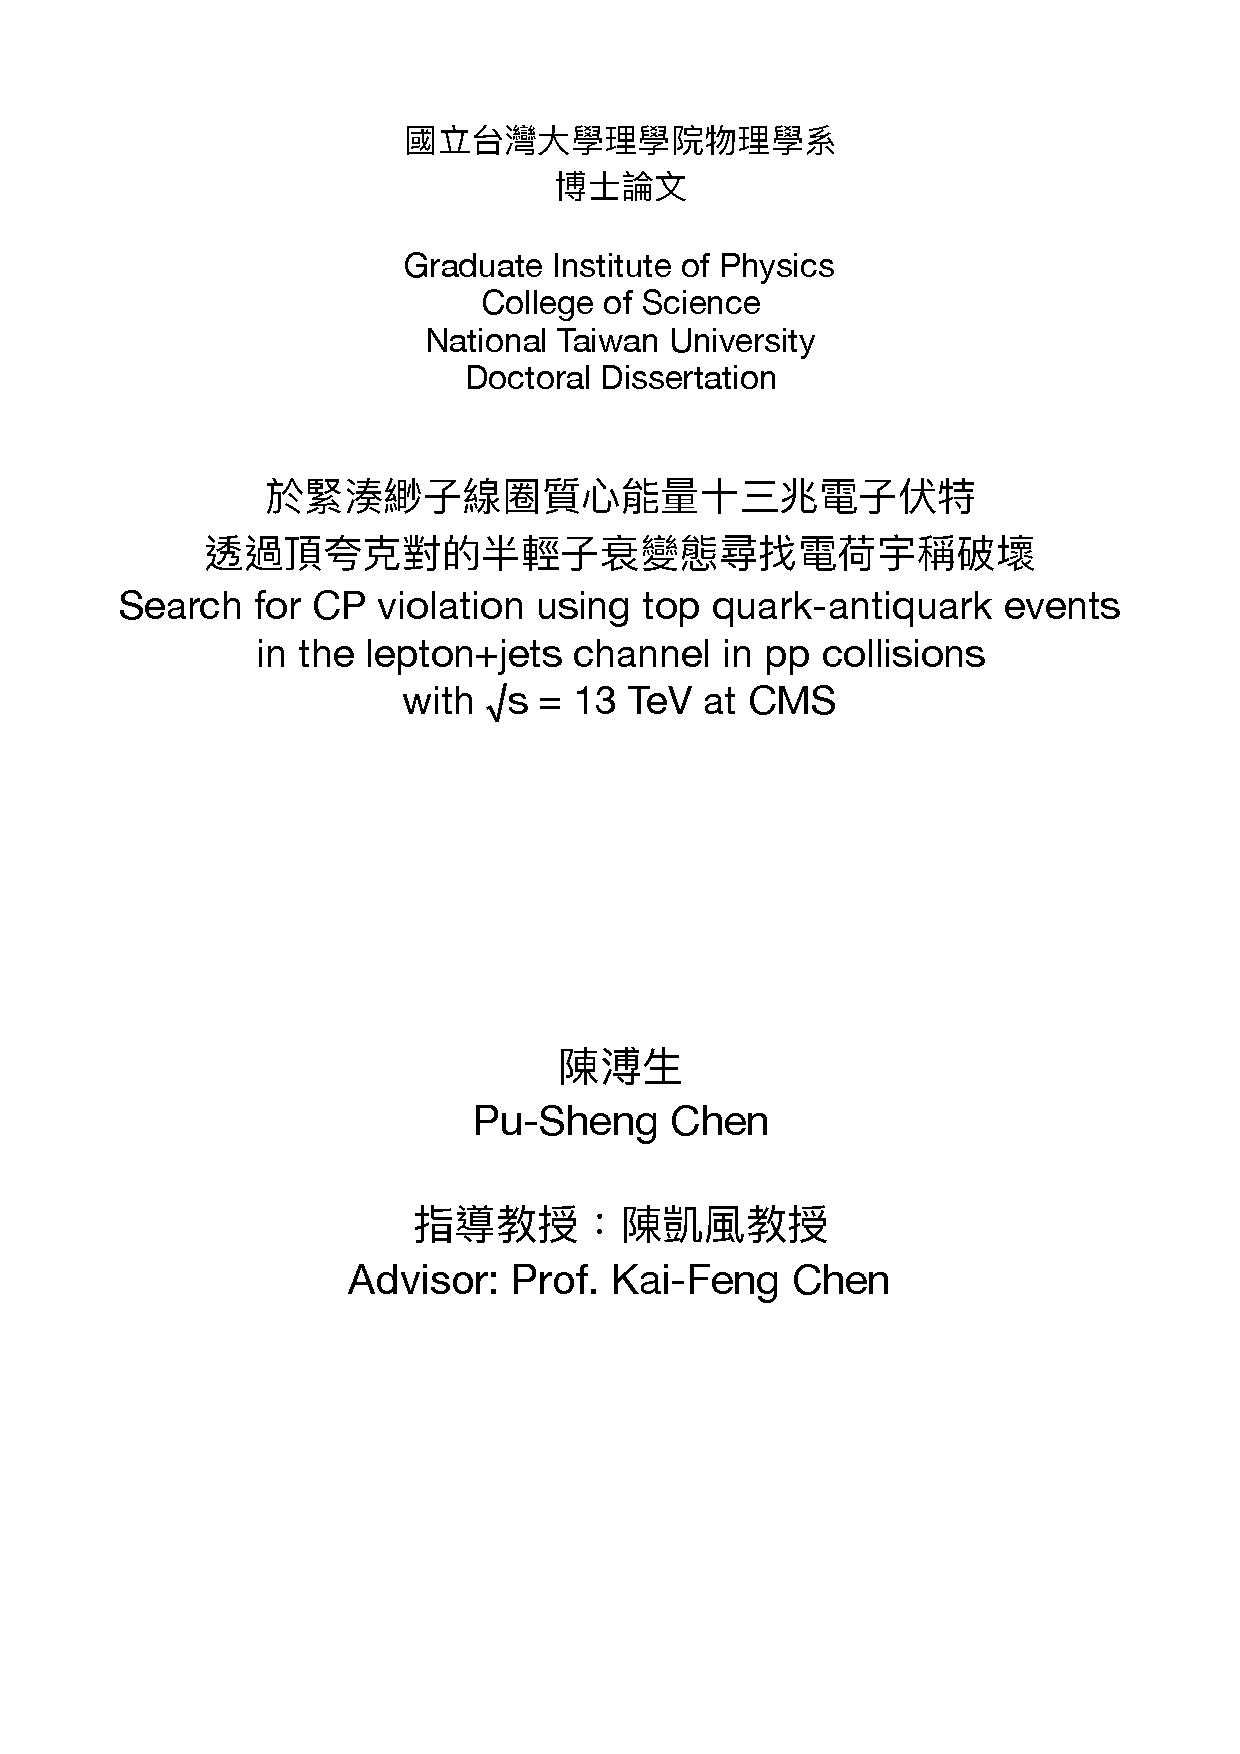
\includepdf[pages=-]{title.pdf}

\begin{CJK*}{UTF8}{bkai}
\chapter*{致謝}
\clearpage
\chapter*{摘要}
此論文透過頂夸克對的半輕子衰變態尋找電荷宇稱破壞。此測量使用從2016年到2018年,藉由緊湊緲子線圈收集的質心能量十三兆電子伏特的質子對撞事件,其總和亮度達到一百三十七逆飛靶。此分析方法使用線性獨立的終態粒子的四維動量所建立的可觀測量來測量可能的宇稱破壞。藉由觀測到的不對稱量所測量到的無因次色電偶極矩量為$0.04\pm 0.10\stat\pm 0.07\syst$,此結果顯示沒有電荷宇稱破壞的徵兆,並吻合標準模型的預測。

\noindent 關鍵字:大型強子對撞機、緊湊緲子線圈、標準模型、電荷宇稱破壞、頂夸克對
\clearpage
\end{CJK*}
\chapter*{Abstract}
Results are presented on a search for CP violation in the production and decay of top quark-antiquark pairs in the lepton+jets channel.
The search is based on data from proton-proton collisions at \newTeV, collected with the CMS detector, corresponding to an integrated luminosity of 138\fbinv. 
Possible CP violation effects are evaluated by measuring asymmetries in observables constructed from linearly independent four-momentum vectors of the final-state particles. 
The dimensionless chromoelectric dipole moment of the top quark obtained from the observed asymmetries is measured to be $0.04\pm 0.10\stat\pm 0.07\syst$, and the asymmetries exhibit no evidence for CP-violating effects, consistent with expectations from the standard model.

\noindent\textbf{Keywords}: LHC, CMS, Standard model, CP violation, \ttbar
\clearpage

\tableofcontents
\raggedbottom
\listoffigures
\listoftables

\chapter{Introduction}
    The standard model (SM) of particle physics predicts the violation of the combined charge conjugation and parity (CP) symmetry that originates from a complex phase in the Cabibbo--Kobayashi--Maskawa matrix~\cite{CPVtop:CKMmatrix1973,CPVtop:CKMmatrix}.
Measurements of CP violation (CPV) in the strange (\PQs), bottom (\PQb), and charm (\PQc) quark sectors conducted over the past few decades~\cite{NA48:1999szy,CPVtop:Bfactories,Pajero:2020dum} have been found to be consistent with the SM expectations.
However, the level of CPV in the SM is insufficient to accommodate the observed matter-antimatter asymmetry in the universe~\cite{CPVtop:RevParticlePhy}, motivating searches for sources of CPV beyond the SM (BSM).
In contrast to the \PQs, \PQc, and \PQb quark sectors, CPV in the top (\PQt) quark sector is relatively unexplored.
In the SM, the CPV effects in top quark pair (\ttbar) decays are expected to be small due to the large mass of the top quark in comparison with the other quarks, leading to the Glashow--Iliopoulos--Maiani cancellation~\cite{Glashow:1970gm}.
Thus, any observed CP-violating asymmetry would indicate the presence of BSM phenomena~\cite{CPVtop:CPVinTOP}.
For example, a nonzero chromoelectric dipole moment (CEDM) of the top quark~\cite{CPVtop:8TeVRef,CPVtop:13TeVRef,CPVtop:Tevatron,CPVtop:CPVsource} can generate sizable CPV in the production of \ttbar.
Previous studies performed by CMS in data from \pp collisions at \oldTeV~\cite{CPVtop:CMSresult} found the CP-violating asymmetries (\Acp) in the \ttbar lepton+jets channel to be consistent with the SM prediction.

This paper presents the results of new searches by the CMS Collaboration for CP-violating asymmetries in \ttbar events using the lepton+jets channel from \pp collisions produced at the LHC.
A possible source of CPV at the top quark production and decay vertices arises from BSM interactions through the CEDM of the top quark.
In a model with contributions from a CEDM~\cite{CPVtop:13TeVRef}, the magnetic and electric couplings between top quarks and gluons (\Pg) are conventionally written as
\begin{linenomath}\begin{equation}\label{eq:lagrangian}
    \mathcal{L}=\frac{\SCC}{2}\PAQt\SUTG\sigmn(\CMDM+i\gamma_5\dtg)\PQt\GFST,
\end{equation}\end{linenomath}
where \SCC and \GFST are the strong coupling constant and the gluon field strength tensor, respectively; \PQt and \PAQt are the wavefunctions of the top quark and antiquark; \SUTG are $SU(3)$ generators; \sigmn is defined by the operator $\frac{i}{2}[\gamma^\mu, \gamma^\nu]$; \CMDM refers to the parameter of the chromomagnetic dipole moment; and \dtg is the CP-odd CEDM.
From Ref.~\cite{CPVtop:13TeVRef}, \dtg can be converted into a dimensionless CEDM parameter \dtG as
\begin{linenomath}\begin{equation}\label{eq:cedm_conversion}
    \dtg = \frac{\sqrt{2}v}{\Lambda^2}\text{Im}(\dtG),
\end{equation}\end{linenomath}
where $\Lambda$ is a high-mass scale of the BSM phenomena and $v$ is the vacuum expectation value for the Higgs boson field ($v \approx 246\GeV$).
Higher \dtG values are expected to yield larger \Acp contributions.

In the lepton+jets channel, one of the top quarks is presumed to decay into a bottom quark and a \PW boson that subsequently decays into quark pairs (\qqbar).
The other top quark is required to decay into a bottom quark and a \PW boson that decays leptonically into an electron or muon and its associated neutrino.
We will refer to this as the leptonically decaying top quark.
The analysis exploits four T-odd observables, where T is the time-reversal operator, as proposed in Ref.~\cite{CPVtop:13TeVRef}.
The CP observables are chosen to come from reconstructable final-state objects that can be well measured.
For example, some observables have been discarded because they need the momentum of the leptonically decaying top quark, which is not experimentally measured.
The CP observables take the form $\vec{v_1} \cdot (\vec{v_2}\times\vec{v_3})$, where $\vec{v_i}$ are spin or momentum vectors and $i=1\text{--}3$~\cite{CPVtop:8TeVRef,CPVtop:13TeVRef,CPVtop:Tevatron}.
These triple-product observables are odd under CP transformation if CPT is conserved.
The four CP observables measured in this analysis are defined as
\begin{linenomath}\begin{equation}\begin{aligned}
    \Othree &= \Qell\epsilon(\momB,\,\momAB,\,\momL,\,\momJ) \propto \Qell\vecB^\ast\cdot(\vecL^\ast\times\vecJ^\ast),\\
    \Osix &= \Qell\epsilon(P,\,\momB-\momAB,\,\momL,\,\momJ) \propto
    \Qell(\vecB-\vecAB) \cdot (\vecL\times\vecJ),\\
    \Otwelve &= q\cdot (\momB-\momAB)\epsilon(P,\,q,\,\momB,\,\momAB) \propto (\vecB-\vecAB)_z \cdot (\vecB\times\vecAB)_z,\\
    \Ofourteen &= \epsilon(P,\,\momB+\momAB,\,\momL,\,\momJ) \propto (\vecB+\vecAB)\cdot(\vecL\times\vecJ).
\end{aligned}\end{equation}\end{linenomath}
The symbol $\propto$ indicates that the CP observable is proportional to the triple product; the asterisk symbol represents the quantity measured in the center-of-mass frame of the $\bbbar$ pair, where \PAQb indicates the \PQb antiquark; $\epsilon(a,b,c,d) \equiv \epsLC a^\mu b^\nu c^\alpha d^\beta$, where \epsLC is the Levi--Civita tensor; $P$ and $q$ are the sum and difference of the four-momenta of the protons in the \pp collision, respectively; \momB and \momAB refer to the two \PQb jet momenta, where the \PQb jet definition will be given below; \momL is the momentum of the lepton (\Pell) that originates from the \PW boson decay; \momJ refers to the momentum of the highest transverse momentum (\pt) jet from the hadronically decaying \PW boson; \Qell is the charge of the lepton; and the $z$ subscript indicates a projection along the beam axis in the CMS coordinate system.

The tabulated results are provided in the HEPData record for this analysis~\cite{hepdata}.
The paper is organized as follows.
Section~\ref{sec:detector} introduces the basic features of the CMS detector.
Section~\ref{sec:selection} provide information on the data, simulations, and selection criteria.
Sections~\ref{sec:fitresult} and~\ref{sec:uncertainty} describe the fitting procedures, the instrumental effects, and the resulting systematic uncertainties.
The final results are presented in Section~\ref{sec:results}, with a brief summary given in Section~\ref{sec:summary}.

\chapter{Experimental Apparatus}\label{sec:detector}
    The Large Hadron Collider (LHC) is the largest and most powerful particle collider in the world.
It is constructed by the European Organization for Nuclear Research (CERN) between 1998 and 2008 in collaboration with 10 000 scientists and engineers from over 100 countries and 1000 research institutes.
The LHC provides proton beams circulating in oppositie directions and colliding at high energy.
Those proton-proton collisions happen at specific interation points, where particle detectors are situated.
The Compact Muon Solenoid detector (CMS) is one of these detectos.
It is built as the joint efforts of nearly 4000 individuals from over 40 countries and 200 research institutes.
The physical quantities of particles emitting from the proton-proton collisions can be well measured by the CMS detector.

    \section{Large hadron collider}
    \begin{figure}[H]\centering
    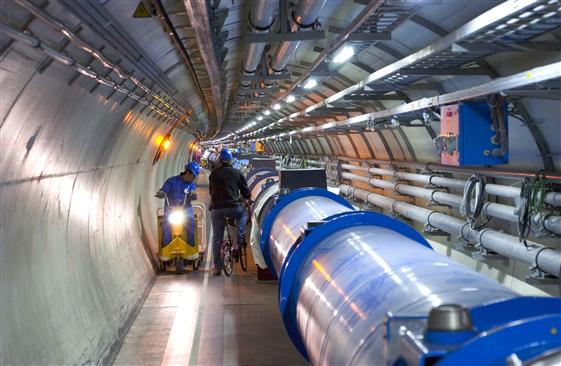
\includegraphics[width=0.6\textwidth]{figure/lhc_tunnel.jpg}
    \caption{LHC tunnel and beam pipe.}
    \label{fig:lhc_tunnel}
\end{figure}
The LHC lies in the already existing 27 km tunnel (Fig.~\ref{fig:lhc_tunnel}) which previously hosted the Large Electron Positron collider (LEP) in the Geneva region and it is as deep as 175 m  beneath the France-Switzerland boarder.
The LHC yields head-on collisions of 7 \TeV for proton-proton beams and the collision energy reach to 13 \TeV with a designated luminosity of $2 \ten{34}$\percms in the LHC RunII period (2015 - 2018).
The prime motivaition of the LHC is to test the predictions of different theories of partilce physics, and have the ability to explore rare evetns such as the Higgs boson production and physics beyond the SM. 

\subsection{Proton injection and operational cycle}
The proton beams goes through series of stages of acceleration (Fig.~\ref{fig:lhc_layout}) to achieve the desired collision energy.
Protons are first produced by linear particle accelerator (LINAC2).
The LINAC2 provides bottles of negative hydrogen ions as the source of the protons, and the electrons are stripped from the hydrogen ions by the electric field leaving only the nucleus containing one proton.
The protons are then boosted up to 50 \MeV, feeding the Proton Synchrotron Booster (PSB) which is the first accelerator in the acceleration chain.
The protons are further speeded up to 1.4 \GeV by four superimposed rings with a radius of 25 m inside the PSB.
The Proton Synchrotron (PS) with 277 conventional (room-temperature) electromagnets can operates the acceleration up to 25 \GeV and provide the bunches with 25 ns to the Super Proton Synchrotron (SPS).
The SPS is the second largest machine in CERN’s accelerator complex, and have the ablility to boost the protons from the PS up to 450 \GeV before they are injected into the main accelerator with the designated energy of 6.5 \GeV
\begin{figure}\centering
    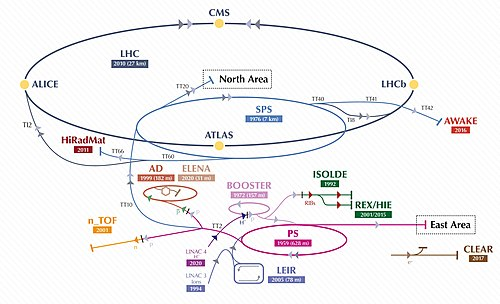
\includegraphics[width=0.8\textwidth]{figure/lhc_layout.jpeg}
    \caption{Schematic layout of the LHC at CERN.}
    \label{fig:lhc_layout}
\end{figure}

\subsection{Machine design}
The LHC contains two adjacent parallel hadron accelerator ring each containing a beam traveling in opposite directions and surrounded by a common cold mass and cryostat, as shown in Fig~\ref{fig:lhc_xsec}.
To avoid the accelerated protons colliding with the air molecules, the pressure in these pipes is \ten{-10} to \ten{-11} mbar, a vacuum almost as rarefied as that found on the surface of the Moon.
Those two rings are designed as twin-aperture magnets containing two contra-rotating beams because of the space limitation in the tunnel.
The beams intersect at four points around the ring, which is where the particle collisions take place.

The LHC is mainly comprised of superconducting magnets and radiofrequency (RF) cavities.
There is about 10 000 superconducting magnets are installed having a mass of over 27 tonnes and all are electromagnets.
A total 1232 main dipole magnets, each 15 meters long, are used to keep the high-energy proton beam on their circular path with a powerful magnetic filed of 8.3 T.
Each dipole magnet is driven by superconducting coils composed of NbTi/Cu rutherford cables.
Approximately 96 tonnes of superfluid helium is needed to keep the magnets at their operating temperature of 1.9 K.
A total 392 quadrupole magnets are allocated symmetrically around the beam pipe to steer the beam in the transverse plane.
To maximize the chances of particle collisions, strongerr quadrupole magnets are used close to the intersection points.
Magnets of higher multipole orders are used to correct smaller imperfections in the field geometry. 
\begin{figure}\centering
    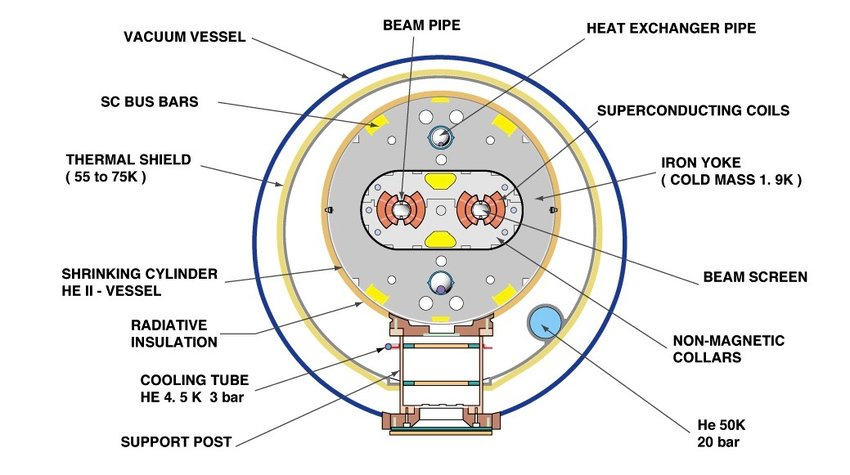
\includegraphics[width=0.8\textwidth]{figure/lhc_xsect.jpg}
    \caption[Cross section of the cryostat system.]
    {Cross section of the cryostat system, where the dipole magnets are surrounded by the superfluid helium.}
    \label{fig:lhc_xsec}
\end{figure}

There are 8 RF cavities per beam pipe on the LHC with a purpose of accelerating the charged particles.
The 16 RF cavities on the LHC are housed in four cylindrical refrigerators called cryomodules which keep the RF cavities working in a superconducting state, without losing energy to electrical resistance.
A RF cavity is a metallic chamber structured like beads on a string, where the string is the beam pipe and the beads are the cavities, shown in Fig~\ref{fig:rf_cavities}.
Each RF cavity is operated with an RF power generator supplying an electromagnetic filed generated from high-power klystrons (tubes containing electron beams).
In order to build up the electromagnetic waves inside the cavity, the RF cavity is molded to a specific shape and size.
The high-power electron beam is extracted through a rectangular pipe of conducting metal called a waveguide, which leads to the RF cavity.
Charged particles passing through the cavity feel the overall force with same direction where the accelerating electromagnetic field oscillates.
It is important to time the arrival of particles since the electromagnetic field is made to oscillate at 400 MHz.
The ideally time proton, with the exact desired energy, will have zero accelerating voltage.
In contrast, protons with slightly different energy from the designated collision energy will be accelerated or decelerated in order to reach to the desired energy and form the proton packs called bunches.
Their accelerating electromagnetic fields can achieve a maximum voltage of 2 MV per cavity (total 16 MV per beam) in the longitudinal direction.
During the energy-boosting process, each injection beam is at 450 \GeV and can be boosted up to top energy in around 15 minutes.
The protons in the bunches have an overall acceleration on each passage through the cavities, and the bunches having passed the cavities around 1 million times at 6.5 \GeV.
\begin{figure}\centering
    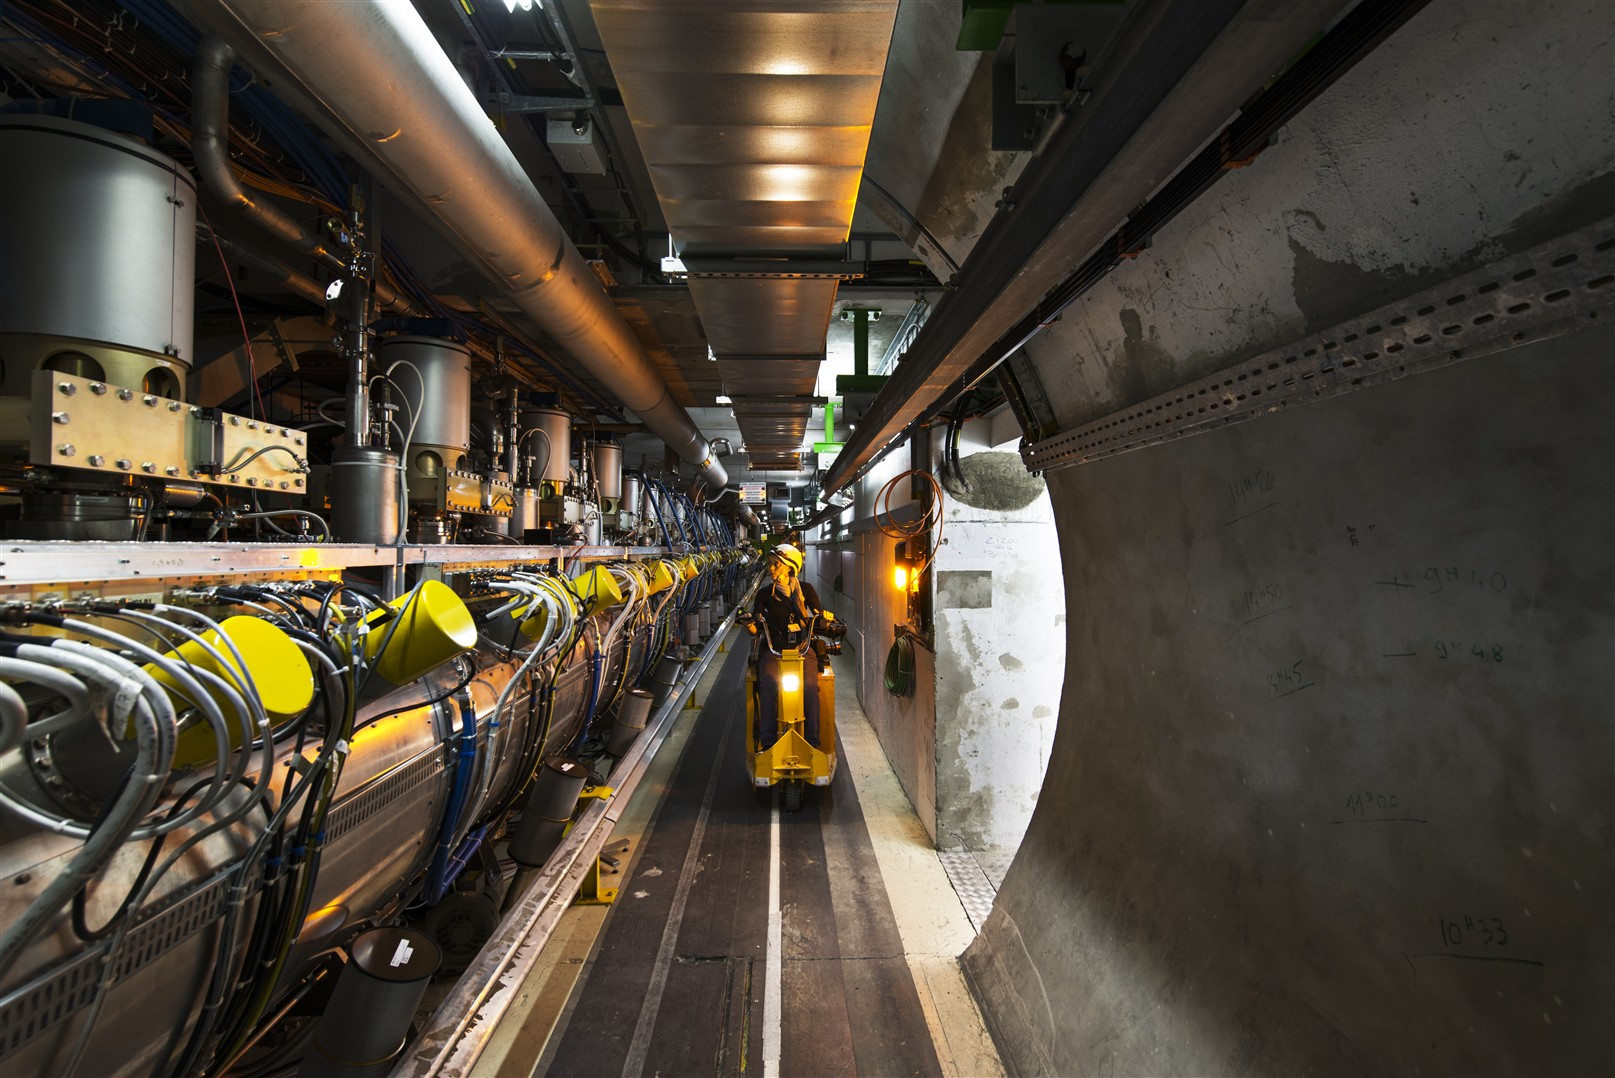
\includegraphics[width=0.8\textwidth]{figure/rf_cavities.jpg}
    \caption{One of the module containing the accelerating cavities for the LHC.}
    \label{fig:rf_cavities}
\end{figure}

The main accelerator is composed of eight arcs and eight straight sections (Fig.~\ref{fig:lhc_arc}).
Either an experimental or utility insertion is located in each straight section.
The two high luminosity experiment, A Toroidal LHC Apparatus (ATLAS) and CMS, are located at Point 1 and Point 5, respectively.
The other experiments, LHC-beauty (LHCb) and  A Large Ion Collider Experiment (ALICE), are located at Point 2 and Point 8, separately.
The utilities containing collimation systems to reduce quenching of superconducting magnets and damage of accelerator components are based on Point 3 and Point 7.
The RV cavity systems for particle acceleration and beam dumping system extracting beams from each ring of the collider can be found at Point 4 and Point 6, respectively.
\begin{figure}\centering
    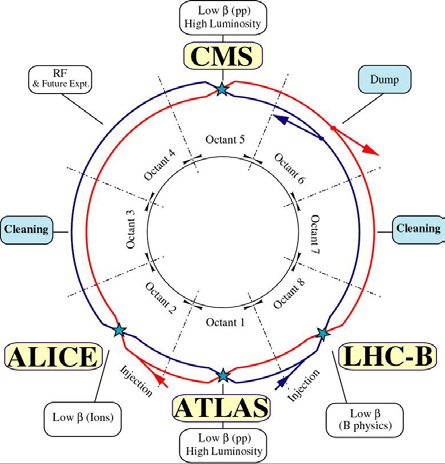
\includegraphics[width=0.5\textwidth]{figure/lhc_arc.png}
    \caption{Schematic layout of the main accelerator for the LHC at CERN.}
    \label{fig:lhc_arc}
\end{figure}

\subsection{Luminosity and pileup}
Luminosity gives a measure of how many collisions are happening in a particle accelerator.
It is an important indicator to reflect the number of collisions that occur in a given amount of time. 
The higher the luminosity, the more data the experiments can gather to allow them to observe rare processes.
The number of events produced per second from a process can be written as
\begin{linenomath}\begin{equation}\label{eq:lumi_nevt}
    N_X = L_0 \sigma_{\pp\rightarrow X}
\end{equation}\end{linenomath}
where $L_0$ is the instantaneous luminosity, $\sigma_{\pp\rightarrow X}$ is the cross section of the $X$ production, and $N_X$ is the number of events.
With the assumption that the proton beam density function follows a normal distribution and the two colliding beams are with the same beam parameters, the instantaneous luminosity can be defined as
\begin{linenomath}\begin{equation}\label{eq:lumi_l0}
    L_0 = \frac{N^2_b n_b f_{\mathrm{rev.}} \gamma_r}{4\pi\hat{\epsilon}\beta^*}F
\end{equation}\end{linenomath}
where $N_b$ is the number of particles per bunch; $n_b$ is the number of bunches per beam; $f_{\mathrm{rev.}}$ is the revolution frequency; $\gamma_r$ is the relativistic gamma factor; $\hat{\epsilon}$ is the normalized transverse beam emittance; $\beta^*$ is collision point of the amplitude $\beta$ function; and $F$ is the geometric luminosity reduction factor. $F$ can be further expressed as
\begin{linenomath}\begin{equation}\label{eq:lumi_F}
    F = \biggl( 1 + \Bigl(\frac{\theta_c \sigma_z}{2\sigma^*}\Bigr)^2 \biggr)^{-\frac{1}{2}}
\end{equation}\end{linenomath}
where $\theta_c$ is the full crossing angle at the interaction point, $\sigma_z$ is the RMS bunch length, and $\sigma^*$ is the transverse RMS beam size at the interaction point.

The LHC cranks up the performance to achieve high instantaneous luminosity at the cost of pileup (PU).
The PU is defined as the average number of particle interactions per bunch-crossing, and can be expressed as
\begin{linenomath}\begin{equation}\label{eq:lumi_pu}
    \bigl< \mu \bigr> = \frac{\mathcal{L}_{\mathrm{inst.}}\sigma^{\mathrm{inel.}}_{\pp}}{n_b f_{\mathrm{rev.}}}
\end{equation}\end{linenomath}
where $\sigma^{\mathrm{inel.}}_{\pp}$ is the inelastic proton-proton cross section with a value of 69.2 mb at \newTeV and $\bigl< \mu \bigr>$ is the PU.
The value of the PU reflects the number of particles produced at the same time, and high PU presents a challenge for physics analyses to successfully identify collisions of interest resulting from signal processes.

The LHC has delivered more than 160 \fbinv overall of proton-proton collisions in Run 2, and the CMS collected more than $92\%$ of the Run 2 data successfully yielding a total dataset of 150 \fbinv.
Figure~\ref{fig:lhc_lumi} shows the integrated luminosities during the LHC Run I and Run II.
The integrated luminosity for physics analysis from 2016 to 2018 is 137 \fbinv and the instantaneous luminosities are 1.4 \percms in 2016 and 2.1 \percms in 2017 and 2018.
The measured PU distribution in the CMS experiment during the LHC Run 1 and Run 2 is shown in Figure~\ref{fig:lhc_pu}.
The machine reached a peak average pileup of around 60 in 2018.
\begin{figure}\centering
    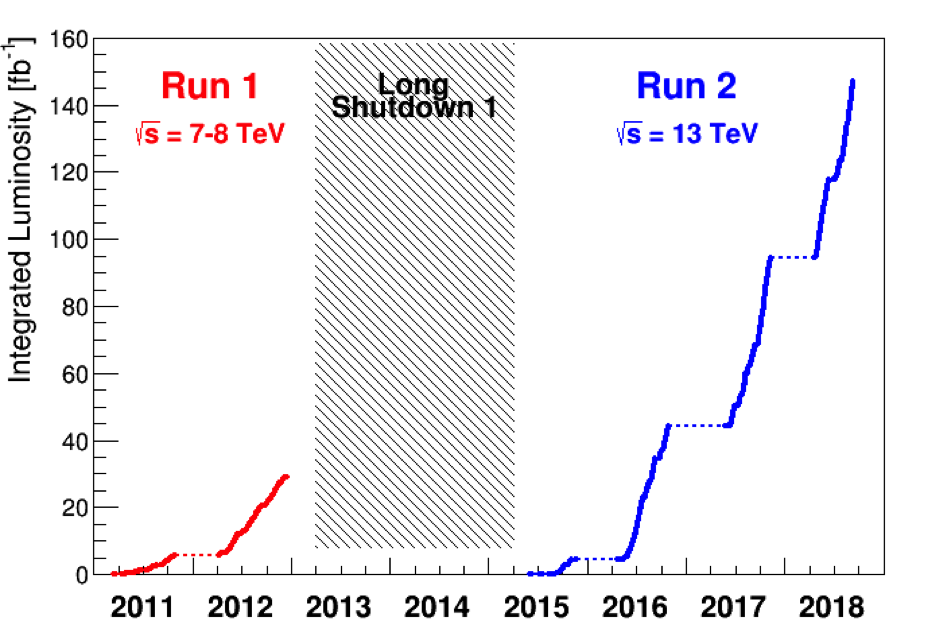
\includegraphics[width=0.5\textwidth]{figure/lhc_lumin.png}
    \caption{Integrated luminosities of Run 1 and Run 2.}
    \label{fig:lhc_lumi}
\end{figure}

\begin{figure}\centering
    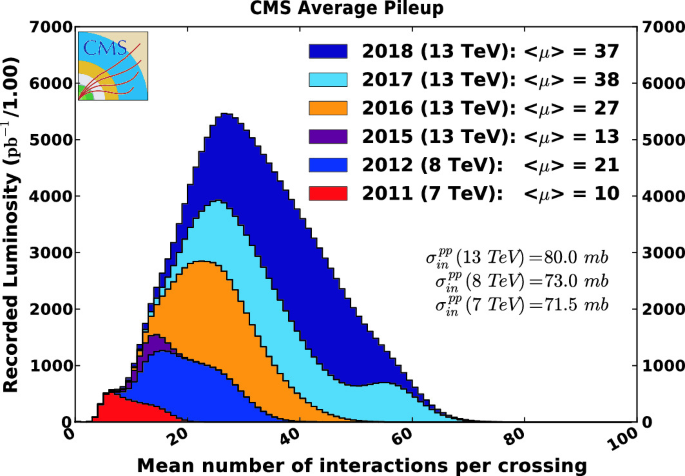
\includegraphics[width=0.5\textwidth]{figure/lhc_pu.png}
    \caption[Average pileup profile for each year of data-taking of the CMS experiment.]
    {Average pileup profile represented in stacked histograms for each year of data-taking of the CMS experiment during the LHC Run 1 and Run 2.}
    \label{fig:lhc_pu}
\end{figure}

    \section{Compact muon solenoid}
    The CMS detector~\cite{Chatrchyan:1129810}, with a very large angular coverage around the interaction points except for the two ends of the beam line, is designed to be a general purpose particle detector.
The CMS detector is composed of solenoid magnet and steel yokes weighting 14,000 tonne, using almost twice much iron as the Eiffel Tower.
The main goal is to detect and measure precise momentum and energy of all stable particles emitting from the proton-proton collisions.

The CMS detector design and layout is driven by an important aspect, the superconducting solenoid providing an average 3.8 T magnetic filed for bending the trajectory of charged particles leaving the interaction point.
The strong but uniform magnetic fileds generated by the solenoid is parallele to the beam direction, while not interfering with the LHC beam operation.
The inner tracking system with a pixel detector and a strip tracker is positioned in the immediate proximinity of the interaction point.
The trajectory (also known as the track) of the charged particles originating from the collision points in the magnetic field can be reconstructed using the small deposits of energy left by the charged particles, while passing through the tracking system.
The energy is small enough that the momentum of the particle could be considered unchanged.
Calorimeters measuring the energy of the specific particles for particle identification are placed outside of the tracking system.
Therefore, the energy of the long-lived particle except for the muons and weakly interacting particles such as neutrinos can be deposited completely into the detector before reaching the solenoid.
Finally, the outermost muon detectors can further give measurements of precise momentum and time resolution of muons which are expected to penetrate all detector components. 

Most detector systems are confined in the region where the magnetic field generated from the solenoid is expected to be uniform, and the trajectory of muons penetrating all detector component is one key characteristic of the CMS detector and thus the name of the detector being the compact muon solenoid.
The layout of the detector can be found in Fig.~\ref{fig:cms_layout}
\begin{figure}\centering
    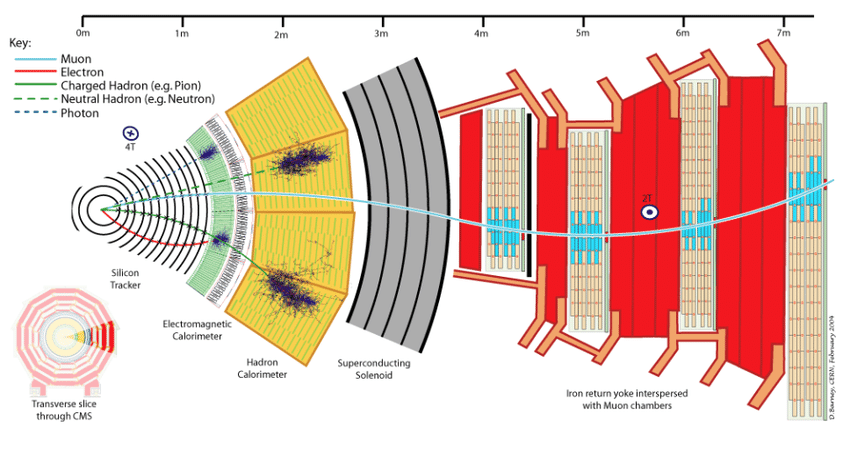
\includegraphics[width=\textwidth]{figure/cms_layout.png}
    \caption{Cross section diagram of the CMS detector and its various subdetector components.}
    \label{fig:cms_layout}
\end{figure}

\subsection{Coordinate system}
The CMS coordinate system is right-handed with its origin at the interaction points, where the $x$-axis points toward the center of the LHC ring, the $y$-axis points to the sky, and the $z$-axis points toward counterclockwise beam direction.
The coordinate consists of the transverse plane, \ie, the $xy$-plane, and the longitudinal $z$-axis.
Due to the cylindrical geometry of the CMS detector, it make sense to use a cylindrical coordinate system, where $\phi$ is an azimuthal angle in the transverse plane and $\theta$ is a polar angle between the $z$-axis, as shown in Fig~\ref{fig:cms_coord}.
\begin{figure}\centering
    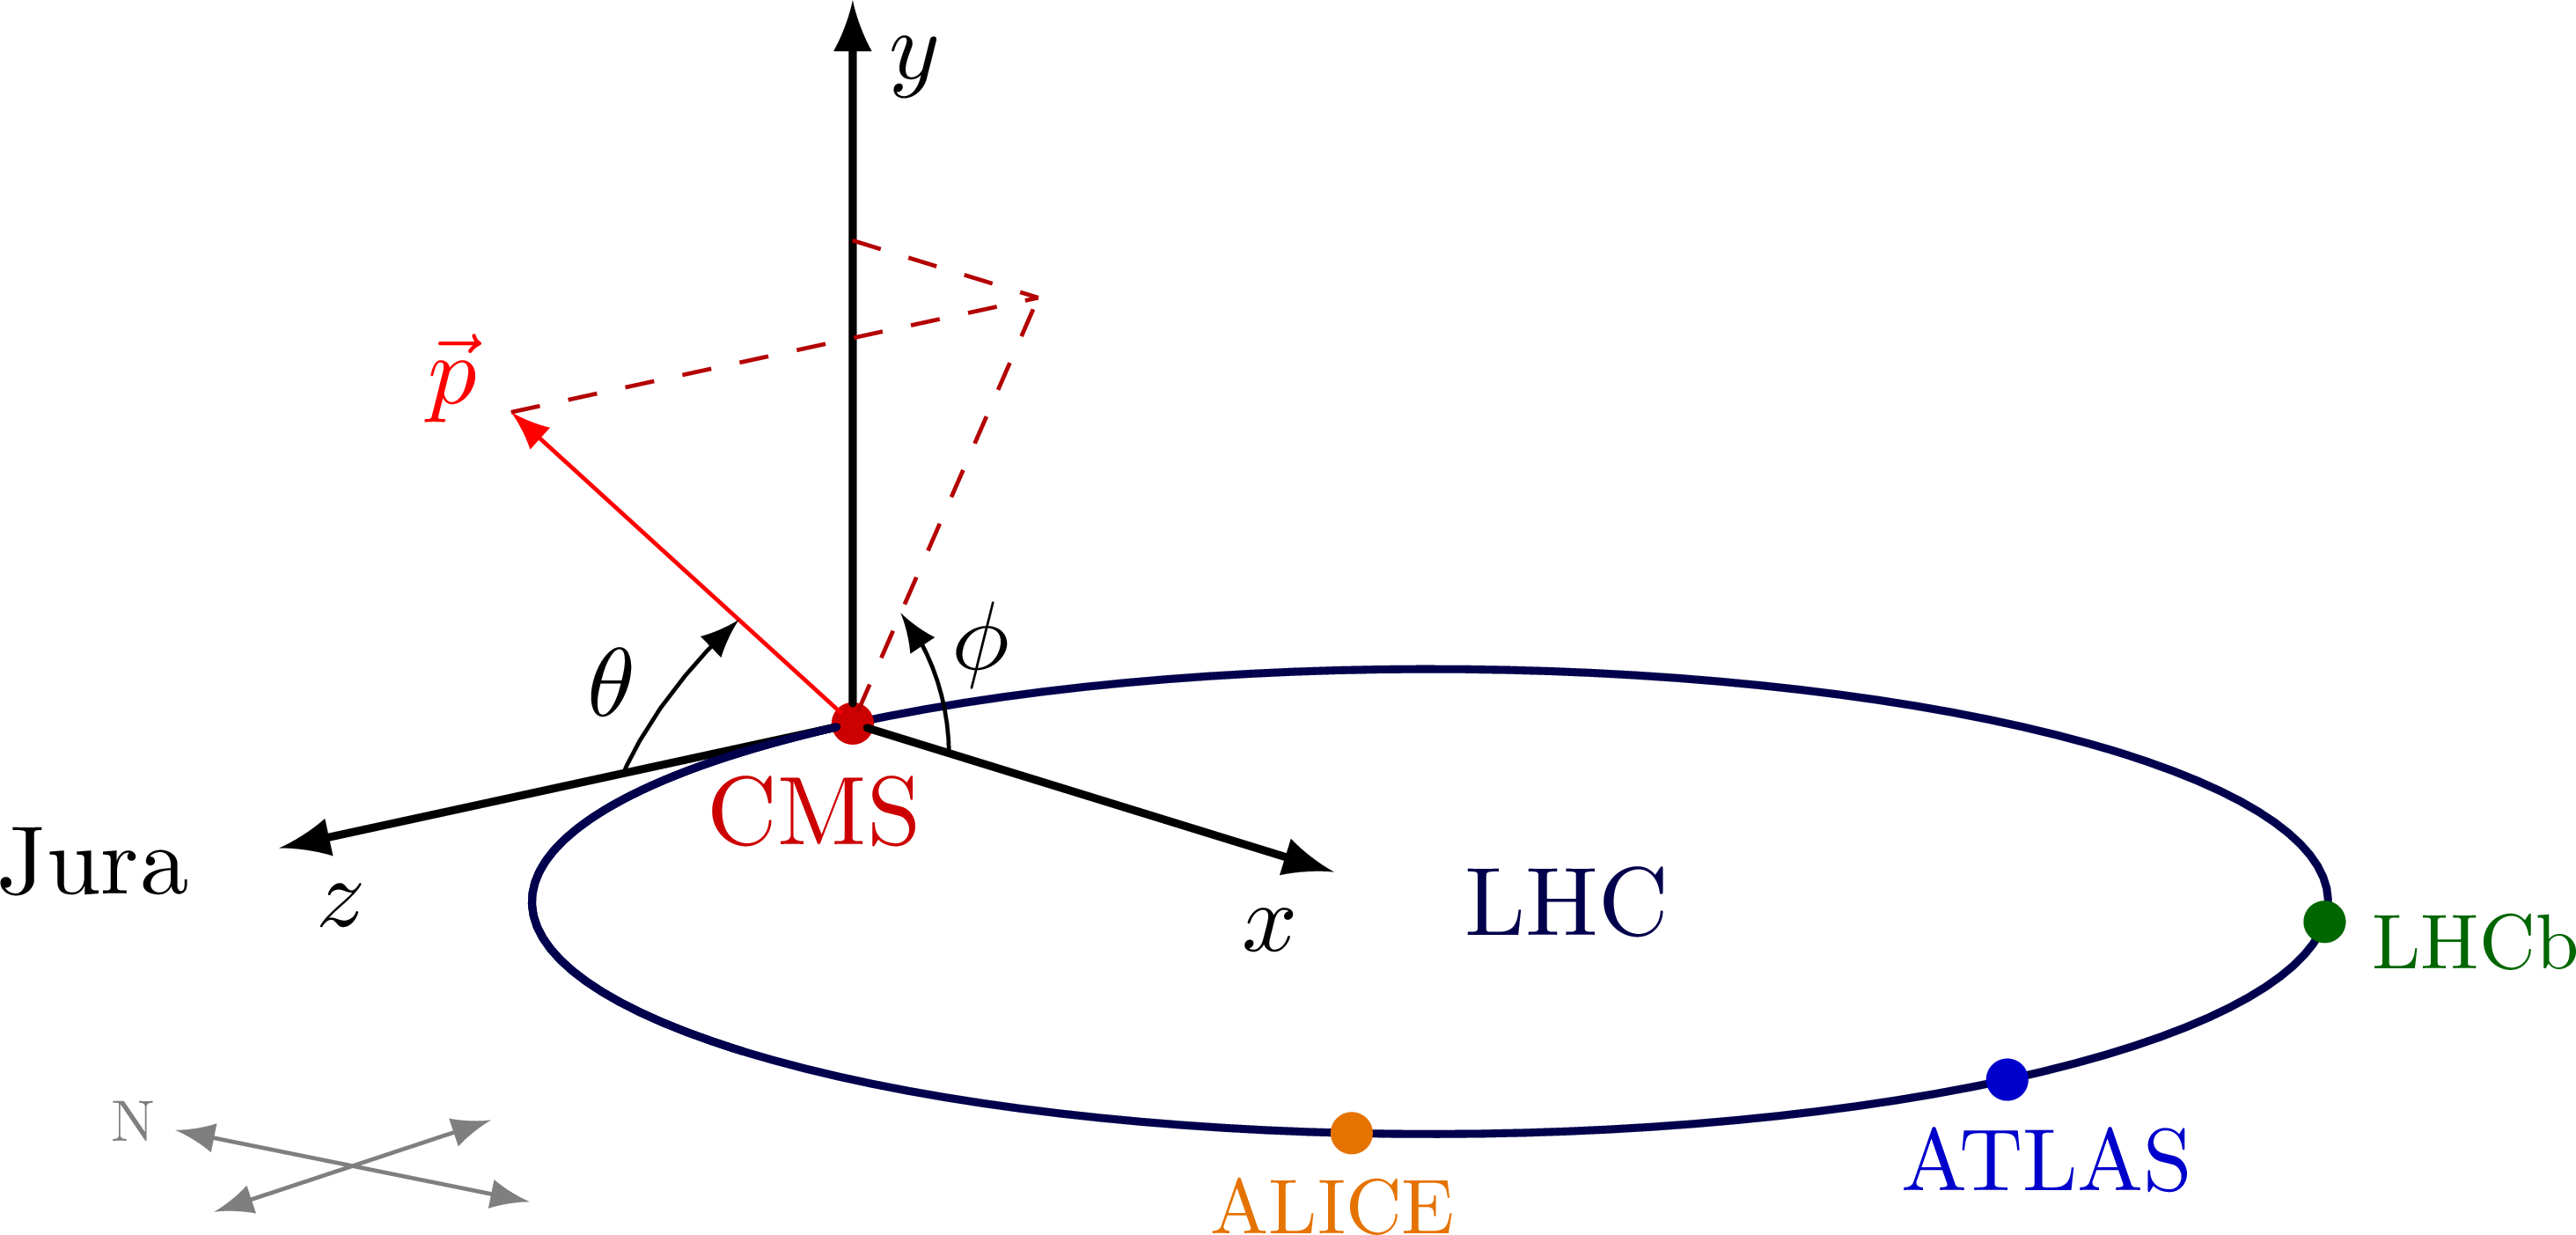
\includegraphics[width=\textwidth]{figure/cms_coord.png}
    \caption{Diagram of the coordinate of the CMS detector.}
    \label{fig:cms_coord}
\end{figure}

Due to the parton density function, the colliding partons carry unknown momenta in the beam direction, even though two protons collide from opposite directions with the same momenta at the $z$ component.
The center of mass of a hard process occurring inside the detector is likely to be boosted along the beam direction.
The polar angle separation $\delta\theta$ between two particles originating from such hard process will not be Lorentz invariant after boosted along the beam direction.
It can be expressed by an Lorentz invariant observable called rapidity as
\begin{linenomath}\begin{equation}\label{eq:cms_rap}
    y = \frac{1}{2}ln \Bigl(\frac{E+p_z}{E-p_z}\Bigr)
\end{equation}\end{linenomath}
Moreover, since the designed interaction energy in the CMS detector is very high compared with the final state particles masses, the rapidity can be further defined as pseudorapidity ($\eta$) with the low mass approximation of $E \rightarrow \vec{p}$.
The pseudorapidity is a function of the polar angle (Fig.~\ref{fig:cms_eta_theta}) defined as
\begin{linenomath}\begin{equation}\label{eq:cms_eta}
    \eta = -ln \biggl(tan\Bigl(\frac{\theta}{2}\Bigr) \biggr)
\end{equation}\end{linenomath}
where $\theta$ is the polar angle.
It is also worth mentioning that the transverse momentum $\PT=\sqrt{p^2_x+p^2_y}$ and $\phi$ are Lorentz invariant under the longitudinal boost.
That is the reason why the four-momentum is described as $(\PT, \eta, \phi, E)$ instead.
\begin{figure}\centering
    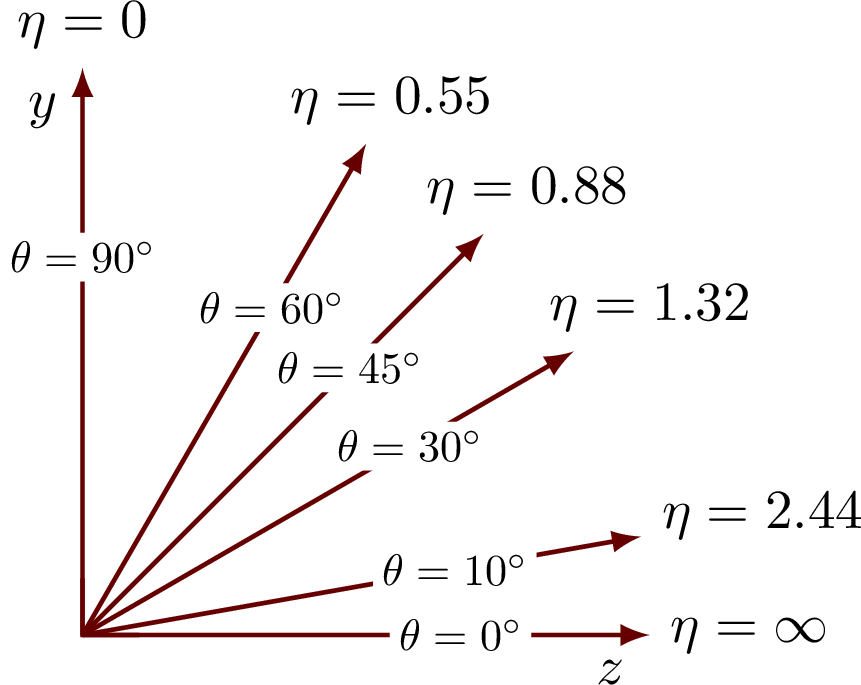
\includegraphics[width=0.7\textwidth]{figure/cms_eta_theta.png}
    \caption{Diagram showing the conversion between $\theta$ (in degrees) and $\eta$.}
    \label{fig:cms_eta_theta}
\end{figure}

\subsection{Tracking system}
The measurement of the momentum of particles plays an important role in helping us to build up a picture of what happens in the collisions.
The transverse momentum, \PT, of a particle can be calculated by tracking its path through a magnetic field as
\begin{linenomath}\begin{equation}\label{eq:cms_momentum}
    \PT = qrB
\end{equation}\end{linenomath}
where $q$ is the electric charge of the charged particle and $r$ is the radius of its trajectory under the magnetic field $B$.
The more curved the path, the less momentum the particle had.
The tracking system is designed to reconstruct the trajectory of charged particles by recording the positions of the small energy deposits left by charged particles passing through the detector components, including high-energy muons, electrons, hadrons, and tracks coming from the decay of short-lived particles such as \PQb quarks.
In order to record particle paths accurately yet with minimum energy loss so as to disturb the particle as little as possible, the trackers use just a few measurement points to reconstruct the tracks.

The measurement is silicon based to resist radiation and is accurate to 10 micrometer, a fraction of the width of a human hair.
The silicon sensors are composed of high does p-type backplane with high reverse bias voltage placed below the bulk which induce electron-hole pairs while high energy charged particles passing through the depletion region.
The electron-hole pairs are carried out to surface through the reverse bias voltage and create a small current which is the signal via additional electronic circuits.
The detector modules composed of silicon-based equipment manufactured on 2D wafers are positioned around the interaction point to have a good coverage of all the particles originating from the collisions.
The final design a tracker consists of the pixels, at the very core of the detector and dealing with the highest intensity of particles, and the silicon microstrip detectors that surround it.
The sensor components in the pixel detectors are manufactured in $100 \times 150 \mu$m cells.
In contrast, the strip trackers are composed of sensor manufactured in 120 - 180 $\mu$m wide strips stretching across an entire module, thus having lower granularity than the pixel detectors.
Though it would be ideal to have full 2D information for each module, it would be practical to lower the power density, which requires more cooling system introducing much more material that would alter the particle trajectory.

\begin{figure}[H]\centering
    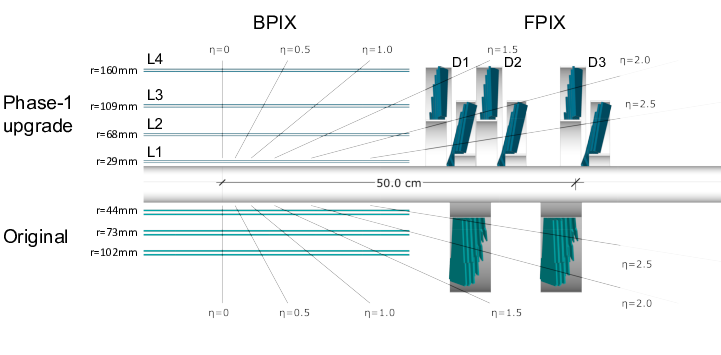
\includegraphics[width=0.9\textwidth]{figure/cms_pixel.png}
    \caption{Arrangement of the Pixel detector after phase 1 upgrade and the original one.}
    \label{fig:cms_pixel}
\end{figure}

The pixel detectors are situated closest to the interaction point and can be separated into two parts, one is composed of three barrel layers (BPix) and the other one is with two endcap disks (FPix).
The layout of the pixel detectors has been modified since the phase-1 upgrade in 2017~\cite{CMSTrackerGroup:2020edz} into four layers in the barrel part and six disks in the endcap part, as shown in Fig.~\ref{fig:cms_pixel}.
The original design can provides 3 tracking points, after the upgrade, the arrangement can further offer 4 tracking points even in high pileup environment.
The BPix having a radial distance of 2.9, 6.8, 10.9, 16.0 cm from the interation points provide high resolution starting points for the algorithm to reconstruct the particle trajectories.
The FPix situated at $|z|$ positions 30.9, 33.8 38.4, 41.3 47.9, 50.8 cm, covering 6.5 cm of radial distance from the beam axis, giving the pixel modules and angular coverage up to $|\eta|<2.5$ around the interaction point.

\begin{figure}[H]\centering
    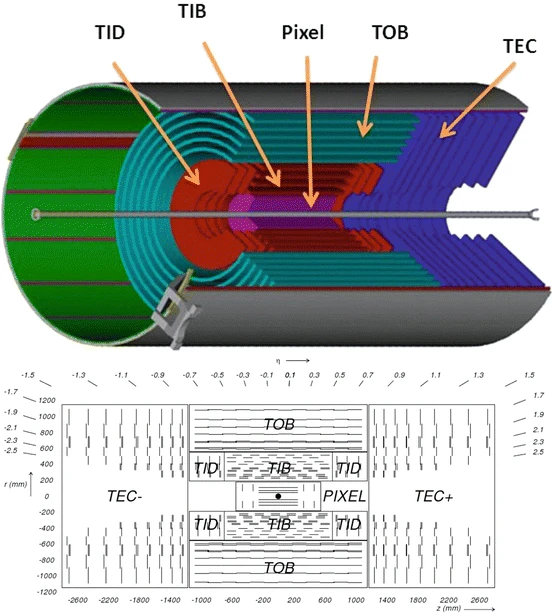
\includegraphics[width=0.8\textwidth]{figure/cms_tracker.png}
    \caption[Schematic overview and $r-z$ view (bottom) of the CMS tracking system.]{
        Schematic overview (top) and $r-z$ view (bottom) of the CMS tracking system.
        The silicon pixel detector in the center is surrounded by the strip detector which consists of endcaps and different barrel components.
    }
    \label{fig:cms_tracker}
\end{figure}
The strip detectors are situated outside the pixel system with 5.5 m in length, 2.4 m in diameter and angular coverage up to $|\eta|<2.5$, as shown in Fig.~\ref{fig:cms_tracker}.
It contains two barrel part occupying a radial coverage from 25.5 to 108.0 cm over the 10 layers of strip modules between the tracker inner barrel (TIB) and the tracker outer barrel (TOB) system, and two endcap part extending the coverage in the $|z|$ directions to 282 cm and angular coverage up to $|\eta|<2.5$ with 13 layers of strip modules between the tracker inner disks (TID) and tracker endcaps (TEC).
There are 9.6 million $p^+$ strips implanted into n-type bulks with 320 $\mu$m thickness inside the strip tracker.
The positive voltage is connected with the n-type backplane of the bulk to produce a reverse bias voltage between the backplane and $p^+$ strip.

\subsection{Electromagnetic calorimeter (ECAL)}
The ECAL detector mounted outside the tracker system is designed to measure the electromagnetic deposit energy of photons and electrons under strong magnetic field.
It is composed of 75 848 homogeneous lead tungstate (PbWO$_4$) crystals with photodetectors, as shown in Fig.~\ref{fig:cms_crystal}.
The photodetectors can capture the signal when the charged particles pass through and excite the crystal atoms, subsequently releasing the excitation energy in narrow frequency photon shower.
Due to the short radiation length (0.89 cm), small Molière radius (2.2 cm), the lead tungstate is chosen as the scintillating crystal to provide high energy resolution and granularity for ECAL.
Moreover, the lead tungstate can provide high time resolution with very short decay time ($80\%$ of the lights released within 25 ns and $99\%$ is collected in 100 ns) to avoid event overlapping with signals.
However, the scintillation rate of the lead tungstate highly depends on the temperature.
Crystals must be maintained at the designated operation temperature of $18^{\circ}$ within a $0.1^{\circ}$ temperature range.
\begin{figure}\centering
    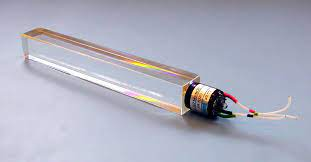
\includegraphics[width=0.8\textwidth]{figure/cms_crystal.jpeg}
    \caption[Photogram of a homogeneous lead tungstate crystal in the EE.]
    {Photogram of a homogeneous lead tungstate crystal in the EE, where the end of the crystal is a vacuum phototriode (VPT) photodetector.}
    \label{fig:cms_crystal}
\end{figure}

The ECAL consists of barrel section and two endcap sections assembled pointing towards the interaction point, shown in Fig.~\ref{fig:cms_ecal}.
The barrel section (EB) is composed of 61 200 individual crystals made in long geometries, $2.2\times 2.2\times 23 \mathrm{cm}^3$ covering $|eta|<1.479$.
The crystals allow total internal reflections to guide the scintillation light naturally to the photodetectors with the high refractive index ($n=2.29)$.
Modules are situated with an inner radius of 1.29 m and angular coverage up to $|\eta|=1.479$ in the barrel region.
In the endcap section (EE), the 3662 crystals for each endcap are arranged in a rectangular $x-y$ grid and are made in $3\times 3\times 22\mathrm{cm}^3$ extending the angular coverage up to $|\eta|<3$.
Endcap modules are positioned with the angular coverage of $1.479 < |\eta| < 3.0$. 
These crystals point at a focus 1300 mm beyond the center of the CMS detector, giving off-point angle ranging from 2 to 8 degrees.
The preshower detector (ES) is seated, just before the endcap, at $1.653 < |\eta| < 2.6$.
It is a silicon detector with a lead absorber aimed to enhance the spacial resolution to the endcap ECAL detectors, especially for distinguishing photons from boosted $\pi_0$ whose diphoton decay can be mis-identified with a single photon.
It is worthwhile mentioning that there is a small gap in the barrel-endcap region $|\eta| \in [1.4476, 1.5564]$, where is lack of crystals.
These regions are known to have poor resolution in particle reconstruction, and this region of the detector will not be used for precision measurements.
\begin{figure}[H]\centering
    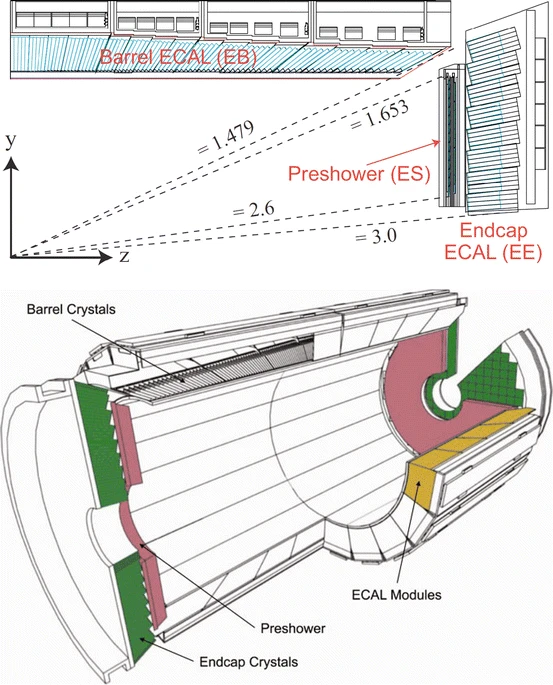
\includegraphics[width=0.7\textwidth]{figure/cms_ecal.png}
    \caption[Schematic view of the ECAL subsystem.]
    {Schematic view of the ECAL subsystem, including the barrel ECAL (EB), endcap ECAL (EE), and preshower (ES) subsystem.}
    \label{fig:cms_ecal}
\end{figure}

During the data collection, the photodetectors, the avalanche photodiodes (APDs) in the EB and vacuum phototriodes (VPTs) in the EE, collect the scintillation light produced from crystals with energy deposited. 
Next, the electronic signals from the photodetectors are amplified by the multi-gain pre-amplifier, which provides three simultaneous analogue outputs digitized at 40 MHz by a 12-bit analog-to-digital converter (ADC).
These digitized and filtered signals are then transmitted to off-detector with Level-1 trigger for further management.
The ECAL performance, the barrel energy resolution~\cite{Adzic:2007mi}, can be measured from an electron test beam experiment and decoupled into three terms as
\begin{linenomath}\begin{equation}\label{eq:cms_ecal}
    \frac{\sigma_E}{E} = \frac{2.8\%}{\sqrt{E(\GeV)}} \bigoplus \frac{12\%}{E(\GeV)} \bigoplus 0.3\%
\end{equation}\end{linenomath}
where the electron energy is reconstructed by the shower in $3\times 3$ crystals.
The first term of the equation is the stochastic term coming from shower containment, number of photoelectrons and fluctuations in the gain process.
The middle term is the noise term contributed by the photodetector electronics.
The last one, the constant term, dominating in high energy photon and electron showers, depends on non-uniformity of the longitudinal light collection, energy leakage from the back of the calorimeter, single-channel response uniformity and stability.

\subsection{Hadronic calorimeter (HCAL)}
The HCAL detector situated outside the ECAL aims to measure the energy of the hadrons and indirectly estimation of the presence of neutrinos.
It is in charge of the reconstruction of the jets originating from quark and gluon fragmentation and hadronization, and is designed as an array of sampling detectors, which strips the energy of the incoming particles with an absorber producing a shower of lower-energy secondary particles.
The scintillating materials then absorb those secondary particles for energy measurements.
The absorber materials used in the CMS detector consists of steel at the very front and back of each tower, and 14 layers of brass in between.
The thickness of the steel layer is 40 mm and 75 mm for the front and back plates, respectively.
The brass layers have a thickness varying from 50.5 mm to 56.5 mm with $70\%$ Cu and $30\%$ Zn, with a radiation length of 1.49 cm and a interaction length of 16.42 cm.

The HCAL detector is separated into the barrel part and the endcap part as with previous subdetector configurations shown in Fig.~\ref{fig:cms_hcal}.
The barrel part (HB) covers $|\eta|<1.4$ composed of 17 layers of active plastic scintillator tiles, giving a granularity of $0.087 \times 0.087$.
The innermost and outermost absorber layers are mode of stainless steel for structural strength.
The effective thickness absorber of the HB are increased with the polar angle from $5.82 \lambda_I$ to $10.6 \lambda_I$.
Since the hadronically interacting particles are not expected to be fully captured by the 17 layers of absorption material, an outer system (HO) placed just outside the solenoid is designed to use the solenoid and magnet iron yokes as an absorption material.
The total effective length can be further extended to a maximum of $11.8 \lambda_I$ in the central region.
The endcap part (HE) with the angular coverage of $1.3 < |\eta| < 3.0$ is with 19 layers of active plastic scintillator, giving granularity of $0.087 \times 0.087$ in $1.3 < |\eta| < 1.74$ and $(0.09 - 0.35) \times 0.087$ in $1.74 < |\eta| < 3.0$.
The average granularity is higher than HB, with a total effective length approximate to $10 \lambda_I$.
The forwards system (HF) is situated further along the beam line at 11.2 m from the center of the CMS detector and covers $3.0 < |\eta| < 5.2$ region.
The HF composed of steel absorbers in a cylindrical structure with radiation hard quartz fibers inserted is designed to measure the particles in the extreme $\eta$ regions.

The HCAL operates when a hadron particle passes through successive layers of absorber producing an amount of secondary particles.
The blue-violet light emitted by these secondary particles passing through the alternating layers of active scintillation is collected by optical wavelength-shifting fibers and shifted into green light.
A green optic signal is then sent by the normal optic cables to the front-end electronics where the optical signal is transformed into fast electronic signals by hybrid photodiodes (HPDs).
The signals are finally sent to data acquisition system for event triggering.
The energy resolution of the combined calorimeter (ECAL and HCAL) can be measured from a test beam experiment~\cite{USCMS:2009fxn} as
\begin{linenomath}\begin{equation}\label{eq:cms_resol}
    \frac{\sigma_E}{E} = \frac{84.7\%}{\sqrt{E(\GeV)}} \bigoplus \bigoplus 7.4\%
\end{equation}\end{linenomath}
where the first term is a stochastic term and the last term is a constant term.

\begin{figure}\centering
    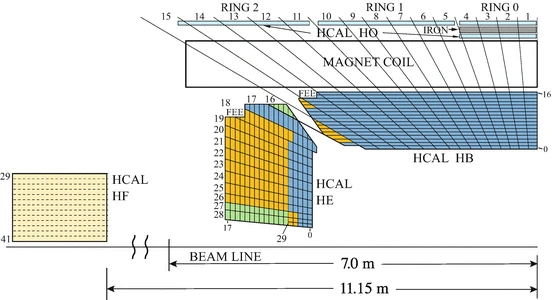
\includegraphics[width=0.9\textwidth]{figure/cms_hcal.png}
    \caption[Schematic view of the HCAL subsystem.]
    {Schematic view of the HCAL subsystem, including the barrel HCAL (HB), endcap HCAL (HE), outer HCAL (HO), and forward HCAL (HF) subsystem.}
    \label{fig:cms_hcal}
\end{figure}

\subsection{Magnet configuration}
The solenoid magnet, which give CMS its last name, is formed by a cylindrical superconducting coils with 6.4 m in diameter and 12.5 m in length making it the largest magnet of its type ever constructed.
It contains four layers of the coils made by Niobium-titanium for its high critical magnetic field and high critical current density.
The coils allows the current of 19.14 kA to flow without resistance while surrounded by 220 tonnes cold mass and cooled down to 4.7k to have no resistance.
The superconducting coils generate 3.8 T magnetic fields inside the detector, including the tracking system and calorimeters.
The job is to bend the paths of charged particle emerging from high-energy collisions for measuring their charges and momenta.

The tracker and calorimeter detectors fit snugly inside the magnet coil whilst the muon detectors are outside the solenoid.
A non-uniform and sparse flux caused by the return magnetic field outside the solenoid could lead ambiguous bending of muons, especially high-energy muons, and worsen the momentum resolution of the muon detectors.
A 12-sided steel flux-return yoke structure with a weight of 12 500 tonne is interleaved between the muon chambers to guide the magnetic and also acts as a filter, allowing through only muons and neutrinos. 
A complete distribution of the magnetic field strength for the magnet is shown in Fig.~\ref{fig:cms_magnet}
\begin{figure}\centering
    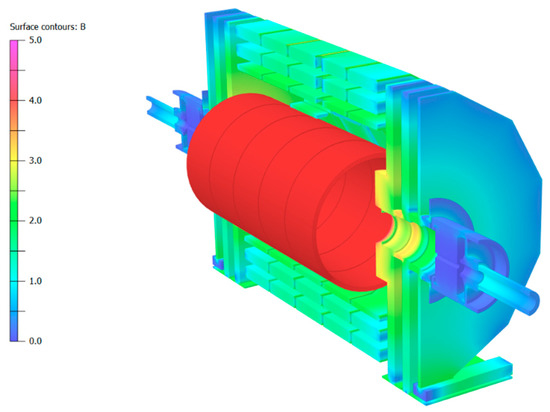
\includegraphics[width=0.8\textwidth]{figure/cms_magnet.jpg}
    \caption[Diagram of the solenoid magnet system in the CMS detector.]
    {Diagram of the solenoid magnet system in the CMS detector with the color scale corresponding to the interval of the magnetic flux density.}
    \label{fig:cms_magnet}
\end{figure}

\subsection{Muon detectors}
Due to the high mass of muons compared with the electrons, the bremsstrahlung radiation is relatively small, and thus muons are expected to penetrate all detector material in the calorimeter system.
Given this unique property, muons are expected to be one of the clearest signature for high energy events.
Precision measurements of muons outside the existing detectors is performed by muon detectors situated outside the outer HCAL system and the solenoid magnet.
A gas-chamber type of detector~\cite{CMS:mu_PF} is designed to reconstruct the muon information with the angular coverage of $|\eta| < 2.4$.
The muon detectors are composed of three different gas ionization chambers, the drift tube chambers (DT), cathode strip chambers (CSC), and the resistive plate chambers (RPC), as shown in Fig.~\ref{fig:cms_muon}.
All the different muon systems share the same sensor operating principle.
The anode and cathode maintained at high voltage differences are interleaved with an inert gas.
Muons passing through this sensor would ionise the gas, which then drift to the anode and cathodes, producing a measurable current at the anode and cathode.
\begin{figure}\centering
    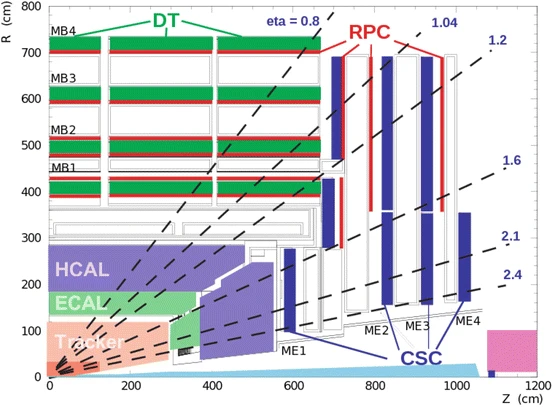
\includegraphics[width=0.7\textwidth]{figure/cms_muon.png}
    \caption[Schematic view of the muon subsystems in the $r-\eta$ plane.]
    {
        Schematic view of the muon subsystems in the $r-\eta$ plane. 
        Cathode strip chambers are in red.
    }
    \label{fig:cms_muon}
\end{figure}


The DTs are placed in the barrel region $|\eta| < 1.2$ where muon rates are expected to be lower, with the basic elements of standard rectangular cells containing four electrodes for shaping the effective drift filed(Fig~\ref{fig:cms_cell}.
The DT cells with a size of 42 mm $\times$ 13 mm $\times$ 2.4 m are layered with the cathode as aluminium tape, and a single gold-plated stainless-stell anode is centered inside each tube shaping the effective drift field with four electrodes.
The anode receives the induced electrons in the inert gas composed of $85\%$ Ar and $15\%$ $\mathrm{CO_2}$ at a drift velocity of about 55$\mu$m/ns when muons go through the cell and ionize the gas.
A DT chamber is made of three superlayers, and a superlayer is composed of three DTs, as in Fig.~\ref{fig:cms_DT}.
\begin{figure}\centering
    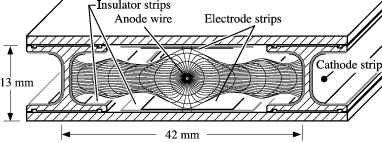
\includegraphics[width=0.8\textwidth]{figure/cms_cell.png}
    \caption[Layout of a DT cell.]
    {Layout of a DT cell, showing the electric field lines in the gas volume.}
    \label{fig:cms_cell}
\end{figure}

\begin{figure}\centering
    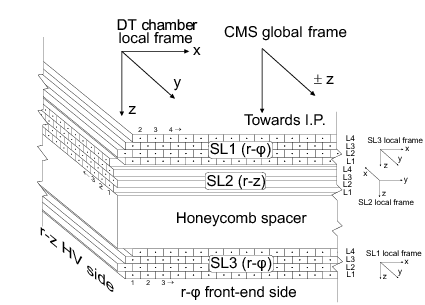
\includegraphics[width=0.7\textwidth]{figure/cms_DT.png}
    \caption[Schematic layout of a DT chamber.]
    {
        Schematic layout of a DT chamber. 
        The SL1 and SL3 superlayers measure the $r-\phi$ coordinate in the bending plane of CMS.
        The SL2 superlayer measures the $z$ coordinate, along the direction parallel to the beam.
    }
    \label{fig:cms_DT}
\end{figure}

Due to the high muon rate and non-uniform magnetic field, the CSC with fast response time is located in the endcaps of the CMS detector.
It covers a region of $0.9 < |\eta| < 2.4$ providing good timing and spacial resolution.
Each CSC consists of 6 anode wire plans interleaved with 7 cathode panels, as shown in Fig.~\ref{fig:cms_CSC}.
The cathode panel are configured as stripes along the radial direction contains 80 cathode strips.
In contrast, the anodes are configured as thin wires with a diameter of 50 $\mu$m on the anode planes along the azimuthal direction.
The anode wire plans are filled with 6 gas gaps in between, each of which is full of a mixture of $50\% \mathrm{CO_2}$, $40\%$ Ar and $10\% \mathrm{CF_4}$.
With the structure mentioned above, the CSCs provide 2 dimensional 2 dimensional information of the muon position within a single chamber module, when the currents of both cathode and anode are measured.
\begin{figure}\centering
    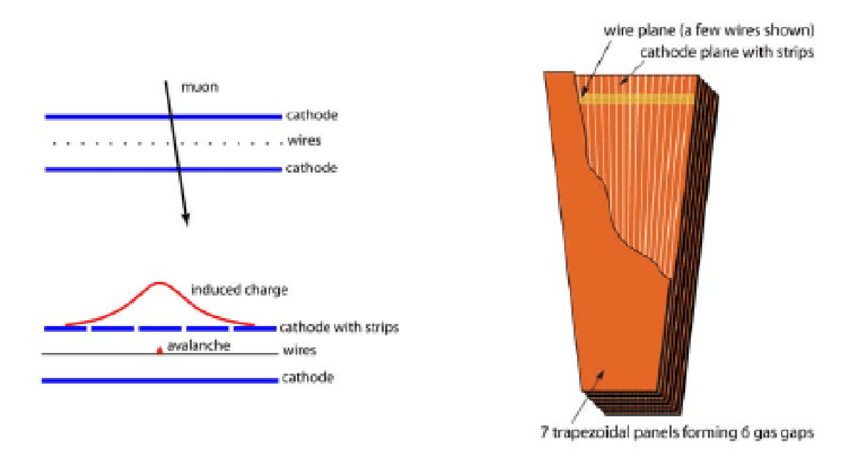
\includegraphics[width=0.85\textwidth]{figure/cms_CSC.png}
    \caption[The layout of CSC system in the CMS.]
    {The layout of a cathode strip chambers (right) and a cross-sectional views of the gas gap in a CSC gap with the anode wires and cathode planes  (left).}
    \label{fig:cms_CSC}
\end{figure}

Besides the DTs and CSCs, the RPC, a trigger-based detector system, is placed outside in both barrel and endcap regions providing adequate timing information for keeping the muon system in sync with the other subdetectors.
Each RPC is made of two gaps composed of highly resistive Bakelite plastic filled with a mixture of $95.2\% \mathrm{C_2H_2F_4}$, $4.5\% \mathrm{i-C_4H_{10}}$ and $0.3\% \mathrm{SF_6}$ in between (Fig.~\ref{fig:cms_RPC}, to keep the drifting electrons and ions from the ionised gases away from the anode and cathode.
The conductive graphite layer on the outer surface of the resistive plates provides avalanches which is sent to the readout strips to form a signal, when charged particles pass through a RPC and ionize the gas.

\begin{figure}\centering
    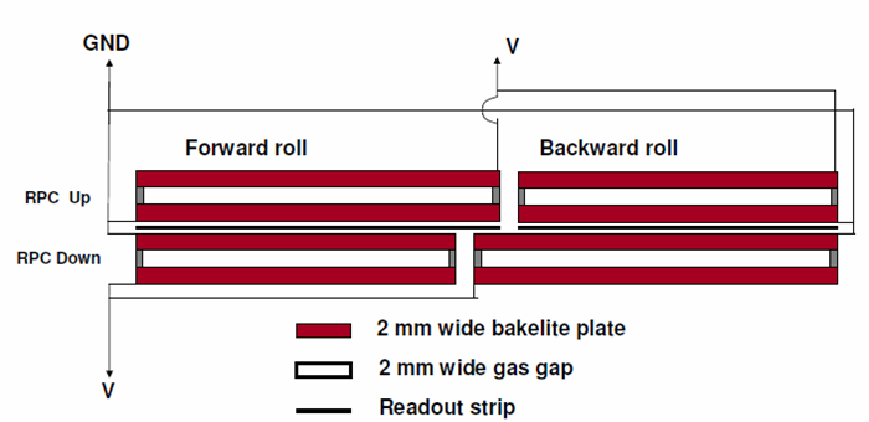
\includegraphics[width=0.85\textwidth]{figure/cms_RPC.png}
    \caption{Schematic view of a generic barrel RPC with 2 roll partitions.}
    \label{fig:cms_RPC}
\end{figure}


    \section{Trigger}
    The LHC provides high-luminosity proton-proton collisions with a maximum bunch crossing rate of 40 MHZ, corresponding to 40 TB/s of data.
Due to the limit of buffer size and disk storage, it is impossible to store such amount of data using prsent day technology.
Trigger system~\cite{Khachatryan:2016bia} are therefore implemented to filter out uninterested events in all the detector readouts, ultimately reducing the event rate to 1 kHz. 
These events are then sent to the CERN tier system for reconstruction and calibration.

\subsection{Level 1 trigger}
A mostly hardware based system called the level 1 trigger system (L1T)~\cite{CMS:2020cmk} is a combination of local and global components (Fig.~\ref{fig:cms_l1t}.
The local trigger systems uses information from a single subdetector, and looks for local patterns such as energy deposit packets, hit patterns, and so on.
The global muon and calorimeter triggers, on the other hand, takes information from corresponding subdetectors and makes very basic reconstruction of physics objects, such as muons, jets, and missing transverse energy to determine whether an event is worth keeping.
The global trigger system then combine information from the local trigger system, and further determines whether an event satisfies the designated requirement.
Once an event meets the requirement of at least one seed, a group of a few criteria, the complete detector information of that event is stored in the front-end buffers and sent to the high level trigger system with a maximal event rate of 100  kHz.

\begin{figure}\centering
    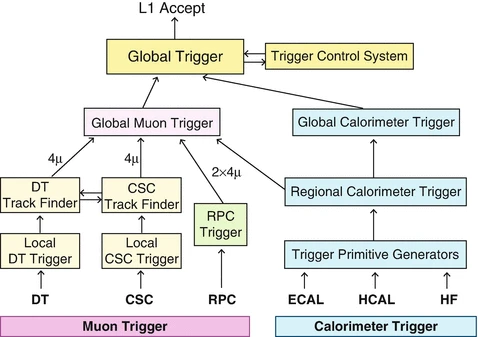
\includegraphics[width=0.85\textwidth]{figure/cms_l1t.png}
    \caption{Architecture of CMS L1 trigger system.}
    \label{fig:cms_l1t}
\end{figure}

\subsection{High level trigger}
In contrast to L1T, The high level trigger (HLT) is entirely software based, and has access to the entire readout data store in the buffer~\cite{CMS:HLT}.
Complex calculations, such as offline reconstruction with filter modules and simple object quality sorting are thus allowed in the software.
Physical quantities like shower shape, isolation and track-vertex can be considered as criteria in the menu.
The data sorting can also take advantage of HLT for quick identification of interesting events, such as the SingleMuon data requiring at least 1 muon HLT o be fired.
The HLT provides higher performancce to identify the interested events and further reduce the event rate from 100 kHz to 1 kHz.

To reduce the amount of common (high cross section) events, such as the production of low energy particles, triggers sometimes record just 1 out of $N$ collisions.
The trigger is said to be prescaled by $N$ with such trigger configuration called prescaling.
The number of events recorded by the detector might be enough for common analysis, however, for searches of rare events, prescaling might decrease the integrated luminosity significantly.

\chapter{Physical object reconstruction}\label{sec:selection}
    The physical objects of interest from the raw digital respons can be reconstructed through the computing process called the particle-flow (PF) algorithm~\cite{CMS:particle_flow}.
The PF algorithm aims to reconstruct and idenrtify stable particles, such as muons, electrons, photon, charged hadrons and neutral hadrons from collision, where ingredients are created from individual subdetector responses, as shown in Fig.~\ref{fig:reco_pf}.
\begin{figure}[H]\centering
    \includegraphics[width=0.95\textwidth]{figure/reco_pf.pdf}
    \caption{Schematic view of a generic barrel RPC with 2 roll partitions.}
    \label{fig:reco_pf}
\end{figure}

These ingredients are joined together with a link algorithm through the expected signatures of particles.
The vertices, tracks and showers are connected with the link algorithm and are identified to some stable particles.
The energy and propagation direction of each stable particle can also be determined.
The corresponding gredients are masked from the list during the following reconstruction, once the target stable particles are reconstructed.
The PF algorithm follows a reconstruction procedure ordered by the level of significant features.
The muon reconstruction is identifed as the top priority, then the isolated photons and electrons, and finally the rest of the non-isolated photon, charged and neutral hadrons.
Bunches of PF candidates are also packed together as jet to represent the short-lived particles that never reach the detector components directly, and particle-based physical objects such as jets missing transverse energy.
This chapter will give an overview of the particle-flow algorithm, focusing on what quantities are especially important to this analysis.


    \section{Particle flow ingredients}
    The ingredients are composed of basic object reconstruction, tracks and clusters.
The reconstruction of chared particle tracks are made using hits on sensitive layers from either tracker system or the muon detector.
The interation points of proton-proton collisions can be build using the positions of reconstructed vertices associated with the reconstructed tracks.
Another basic object, the clusters, can be built using the dedicated clustering algorithm with the position and energy deposited of electromagnetic and hadronic showers from ECAL and HCAL.
\subsection{Track}
The tracks left in the tracking system by charged particles are in a helix structure with 5 degree of freedom: 3 from the particle velocity, 3 from the particle initial position, and -1 from the helix constrain.
The individual hits on the detectors are fitted to an expected track of a particle during the reconstruction.
The sensor elements are triggered when the particles pass the detector modules at certain angle, and the clusters of neighboring sensor elements are joined together as hits.

The weighted average of sensor component coordinates in a cluster can determine the spacial position of hits, which would be further corrected with the incidence angle and corresponding energy deposits when the track is reconstructed.
A dedicated tracking software called the combinatorial track finding (CTF) algorithm which runs several iterations of combinatorial Kalman filter~\cite{Fruhwirth:1987fm} integrating patter recognition and track fitting.
Each tracking iteration is composed of four steps: track seeding, trajectory building, ambiguity resolving, and track fitting~\cite{CMS:2014pgm}.
Figure~\ref{fig:reco_track} shows the tracking efficiency achieves $98\%$ in the CMS experiment.

\begin{figure}\centering
    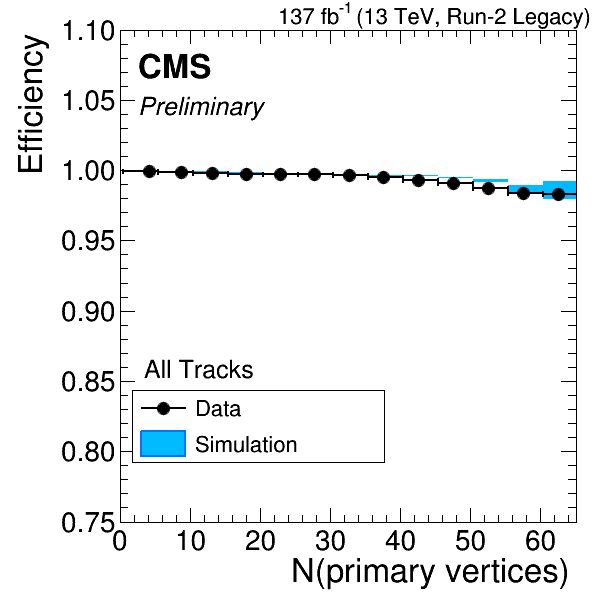
\includegraphics[width=0.5\textwidth]{figure/reco_track.png}
    \caption[The tracking efficiency as a function of the number of primary vertices in the all tracks collection.]
    {
        The tracking efficiency as a function of the number of primary vertices in the all tracks collection. 
        Data (black dots) and \MADGRAPH DY (light blue rectangles). 
        The uncertainties shown are statistical.
    }
    \label{fig:reco_track}
\end{figure}

\textbf{Track seeding} sets the initial trajectory parameters and their uncertainties in the beginning of the reconstruction of a track.
Iconic signatures, for example, the good hits in the pixel detector with close spacial proximity and orientation towards the interaction point are used in the first iterations to give a good estimation of the particle track.
Looser criteria are used in the following iterations to ensure particles decaying in flight in the tracking system is also reconstructed

\textbf{Trajectory building} is commonly referred as the KF process, updating the trajectory parameters at each layer.
It is done by propagating the existing trajectory to the next layer, choosing a hit within a certain neighborhood, and correcting the trajectory parameters from a $\chi^2$ fit.
Multiple additional trajectory candidates are generated when multiple candidate hits exist.
An invalid hit can be an additional information if a particle passes through a detector module without leaving any readout signal, and can be added into the list of hits in the trajectory candidate to indicate where a hit was expected to be.
The procedure is repeated layer by layer until termination conditions, such as poor fitting results (large $\chi^2$, low expected \PT), need for speeding up computations (terminate after finding some consecutive hits), or large number of consecutive invalid hits. 
The hits associated with track candidates can be masked from the list after the first iteration of the trajectory building algorithm.
The process can then restart with a new set of track seeds made with looser seeding criteria.
The CMS performs 5 iterations of the track building with progressively looser criteria for seeding in each iteration for the standard track reconstruction.
This allows particles originating from in-flight decays with as little as 3 hits be constructed.

\textbf{Ambiguity resolving} is then needed to avoid track double counting caused by the multiple trajectory candidates created at each propagation in the trajectory building algorithm.
The track with the larger $\chi^2$ values will be discarded as a duplicate between two track candidate with the fraction of shared hits is greater than $50\%$.

\textbf{Track fitting} reruns the track fitting on the hits among track candidates to reduce biases introduced by the seed selections, and also update the hit information with now-available track information.

\subsection{Vertex}
Vertexing algorithm plays an important role in indicating the physics interaction point by finding the point where trajectories meet.
Primary vertexes close to the beam line and the desired interaction point are expected to be the reconstructed coordinate with large numbers of associated tracks.
Secondary vertexes, in contrast, are points of particles decaying in-flight and expected to have significantly smaller number of associated tracks and a larger transverse distance from the beam line.
Secondary vertexes are collected with subsets of tracks associated with physical objects, and are typically reconstructed only after the primary vertex has been reconstructed.

The results of a $\chi^2$ fit of a vertex position can be done by minimizing a function of sum of standardized distance squared $L(\vec{v})$ as:
\begin{linenomath}\begin{equation}\label{eq:reco_fit}
    L(\vec{v}) = \frac{1}{2} \sum_i \chi^2(\vec{v}, \vec{x_i}) = \sum_i \Bigl( \frac{d_i(\vec{v})}{\sigma_i} \Bigr)^2
\end{equation}\end{linenomath}
where $i$ runs over the indexes of tracks, $d_i(\vec{v})$ is the distance of the vertex position from track $i$, and $\sigma_i$ is the uncertainty in the distance.
However, poorly associated tracks contribute large $\chi^2$ values in this method.
The adaptive vertex fitter~\cite{Fruhwirth:2007hz} sequentially suppresses potentially outlying tacks instead by an additional weighting function:
\begin{linenomath}\begin{equation}\label{eq:reco_weight}
    w(\chi^2) = \frac{\mathrm{exp}(-\chi^2/2T)}{\mathrm{exp}(-\chi^2/2T)+\mathrm{exp}(-\chi^2_c/2T)}
\end{equation}\end{linenomath}
where $T$ is a temperature variable indicating how sensitive the minimization is with large $\chi^2$, and $\chi_C$ is a constant for which $w(\chi_C)=1/2$.
The minimization of Eq.~\ref{eq:reco_fit} can be solved with the weight applied as 
\begin{linenomath}\begin{equation}\label{eq:reco_temp}
    \sum_i w(\chi_i(\vec{x}))\chi(\vec{v})\frac{\partial\chi(\vec{v})}{\partial\vec{v}} = 0.
\end{equation}\end{linenomath}

Then, solve Eq.~\ref{eq:reco_temp} using some augmented function $F(\vec{v})$ instead of $L(\vec{x})$ with the effective $\chi^2$ noted as $\rho(x)$ is give associated
\begin{linenomath}\begin{equation}\label{eq:reco_rho}
    \rho(x) = \frac{1}{2}\chi^2 - Tln\biggl( \frac{1+\mathrm{exp}(\chi^2_C / 2T)}{\mathrm{exp}(\chi^2/2T)+\mathrm{exp}(\chi^2_C/2T)}\biggr).
\end{equation}\end{linenomath}
In the limit of $T\rightarrow 0$, $\rho(\vec{v})$ approaches the original $\chi^2/2$ for $\chi < \chi_C$ and a fixed value for $\chi > \chi_C$ as shown in Fig.~\ref{fig:reco_vertex}.
The minimization of extreme outliers at small $T$ is then expected to be negligible.
The $\chi_C$ is set to 3 in the official operation for reconstructing the primary vertexes because the vertex only has 3 degrees of freedom.
\begin{figure}[H]\centering
    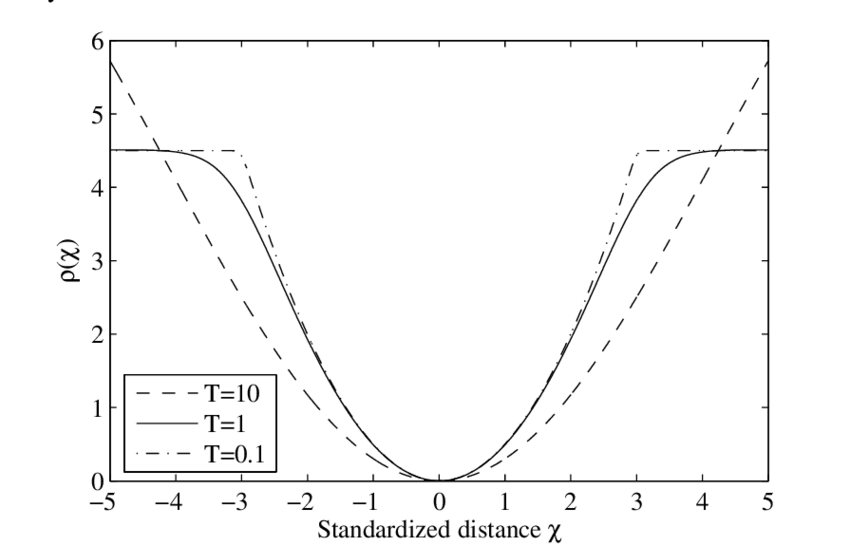
\includegraphics[width=0.5\textwidth]{figure/reco_vertex.png}
    \caption{
        Effective $\chi^2$ function $\rho(\chi)$ at various temperature parameters $T$.
    }
    \label{fig:reco_vertex}
\end{figure}


The initial point of the vertex fitting algorithm is determined by the algebraic mean of the closest point pairs of two tracks.
A weighting value $w=(d+d_{min})^{-1/2}$, where $d$ is the distance of minimal approach, and $d_{min}$ is an offset value of 10$\mu$m then determines the track pair with the largest $w$.
Tracks with small $\chi^2$ are seemed to be associated with the vertex after the vertex is reconstructed.
Tracks without any vertex associated are reiterated to reconstruct primary vertex.

\subsection{Calorimeter clustering}
Clustering algorithms are designed to identify individual particles coming from different physical interactions, while distinguish particles originating from interaction points from particles coming from soft radiation processes.
It is composed of two steps: cluster seeding and topological clustering.

Cluster seeding initialize the clustering algorithm with local maximums which is larger than the expected noise in the calorimeters.

Topological clustering joins particle-flow clusters with neighbor cells with an energy above a certain threshold (80 \MeV in the ECAL barrel, 300 \MeV in the ECAL endcap, and 800 \MeV in the HCAL).
The clustering algorithm has not yet resolved the ambiguity of cells associated with multiple particle-flow clusters at this step.
The cell ambiguity is resolved using the calorimeter granularity after all particle flow clusters has finished the topological clustering process.

    \section{Muon}
    Muons are identified as the top priority in the reconstructed object list.
Besides the globale fit results, a constraint of 3 standard deviation of uncertainty should be satisfied between the momentum of the two tracks.
The tracks are then masked from the ingredient list along with a small subtraction of the expected energy deposits of muons passing through the ECAL (around 3 \GeV) and HCAL (around 0.5 \GeV) system from the clusters laying on the muon trajectory.
The following section will introudce the muon reconstruction and identification in the CMS experiment.

\subsection{Muon reconstruction}
The muon reconstruction is based on track reconstruction since muons leave energy deposits as hits in all subdetectors.
The muon reconstruction in the CMS experiment can be categorized into three different ways:

\begin{itemize}
    \item Standalone muon is reconstructed using hit information from the CSC, DT, and RPC in the muon detector.
        The process begins with track seeding with the DT or CSC segments and then iterate with the KF technique to build the muon tracks.
    \item Tracker muon is made by extrapolating the tracks, with $\PT > 0.5 \GeV$ and a total momentum $p > 2.5 \GeV$, in the tracker system to the muon system with loosely mathcing to the DT or CSC segments.
        The inner track is considered as a tracker muon track if at least one muon segment matching with the extrapolated track.
    \item Global muon is reconstructed by comparing the tracks from standalone muon with tracker system.
        A combined fit is performed by the KF technique to construct a global muon track with information of both the standalone muon tracks and tracks from tracker system, if the parameters of those tracks are matched .
\end{itemize}

Thanks to the high efficiency of the tracker system and muon segment reconstruction, about $99\%$ muons received in the detector acceptance can be successfully reconstructed as tracker muons and global muons,
The tracks can be further merged as a single object if the global muon tracks match to the track muon track.
The associated PF ingredients are then removed from the ingredient list once the muons are reconstructed.

The momentum measurement of muon is performed with a Tun-P algorithm to obtain the precise momentum of muon in different situations.
The algorithm of \PT measurement can be separated into 4 kinds by goodness-of-fit and $\sigma(\PT)/\PT$ criteria:

\begin{itemize}
    \item Inner-track fit uses the information only from the tracker system to determine the momentum.
        The Tune-P algorithm prefers this method for low \PT muons, since the muon detector has less contribution for momentum reconstruction for muons with $\PT < 200 \GeV$.
    \item Tracker-Plus-First-Muon-Station (TPFMS) fit performs a refit to the hits of the global muon track from the tracker system and muon detectors, since the innermost muon detectors give the best muon momentum information among the muon detectors.
    \item Picky fit also takes the hits from the global muon track like TPFMS fit.
        However, it focuses on large hit occupancy such as a shower taking place in the muon chambers.
        In this case, only hits compatible to the extrapolated trajectory based on $\chi^2$ are added into the refit work.
    \item Dynamic-Truncation fit focuses on the case that significantly bent muon trajectory caused by energy loss.
        This method performs a refit with the inner-track extrapolated to the innermost muon detectors and added compatible hits from the segment closest to the extrapolated trajectory.
\end{itemize}

\subsection{Muon identification and isolation}
Muons leave a clear path in both the inner tracking system and muon detectors outside the solenoid.
This iconic signature of muon can be used to determine a great deal of information of the reconstructed muon properties.
The track provides sufficient information in the tracking system with itself being a good fit of the hits and with minimal amounts of invalid hits along the track.

In this analysis, we focus on muons originating directly from a hard scattering process instead of muons coming from secondary decay products of short-lived hadrons.
Therefore, the muon track should be with a primary vertex and occupy all inner tracker system, rather than just a segment.

The muon physics object group defines standard selection criteria for different levels of muon identification (ID) depending on the analysis needs.
A tight muon is required to meet the following criteria:
\begin{itemize}
    \item The candidate is reconstructed as a Global Muon with tracks fitting starting from the muon subdetectors.
   \item Identified by the particle flow algorithm as a muon 
    \item The $\chi^2$/d.o.f of the track fitting should be smaller than 10, at least one muon chamber hit included in the global muon track fit, and muon segments in at least two muon stations.
        These selections suppress hadronic punch-through and muons from decays in flight, that is, suppress accidental track-segment matching, where the inner track might be generated from a particle other than the muon.
    \item The corresponding track having a transverse impact parameter with the primary vertex $d_{xy} < 2$ mm, and a longitudinal distance $d_z < 5$ mm.
        This cut suppress cosmic muons and further suppress muons from decays in flight, while preserves muons originating from the semi-short-lived \PQb and \PQc hadrons.
    \item At least one pixel hit to suppress muons from hadrons decaying in flight.
    \item More than 5 tracker layers hit to guarantee a good \PT measurement.
\end{itemize}

A loose muon, on the other hand, is only required to meet the following criteria:
\begin{itemize}
    \item The candidate is reconstructed as a Global Muon with tracks fitting starting from the muon subdetectors or reconstructed as a track muon.
    \item Identified by the particle flow algorithm as a muon 
\end{itemize}

In order to distinguish prompt muons from the \PW and \PZ bosons decay against those from heavy flavor decays within jets, a particle flow based relative isolation value, noted as $I_{\mathrm{pf,rel}}$, is computed by comparing the momentum of the muon track with the energy deposits in adjacent subsystems and defined as
\begin{linenomath}\begin{equation}\label{eq:reco_muon_iso}
    I_{\mathrm{pf,rel}} = \frac{ \sum p_{\mathrm{T,chhad}} + \mathrm{max}(0, \sum E_{\mathrm{T,neuhad}}  +   \sum E_{\mathrm{T,}\gamma} -  0.5\sum p_{\mathrm{T,pileup}})     }{  p_{\mathrm{T,}\mu} }
\end{equation}\end{linenomath}
where the various $\sum p_{\mathrm{T,x}}$s are the sum of the transverse momentum (or energy) of the charged hadrons, neutral hadrons, photons, and pileup energy within an angular separation $\Delta R < 0.4$ around the muon, and $p_{\mathrm{,\mu}}$ is the transverse momentum of the muon itself.
Designated working points of cut on the $I_{\mathrm{pf,rel}}$ is determined by the muon physics object group.
This analysis choose a tight working point $I_{\mathrm{pf,rel}} < 0.15$ and tight working point ID, giving more than $96\%$ efficiency as shown in Fig.~\ref{fig:reco_muon_eff}.

\begin{figure}\centering
    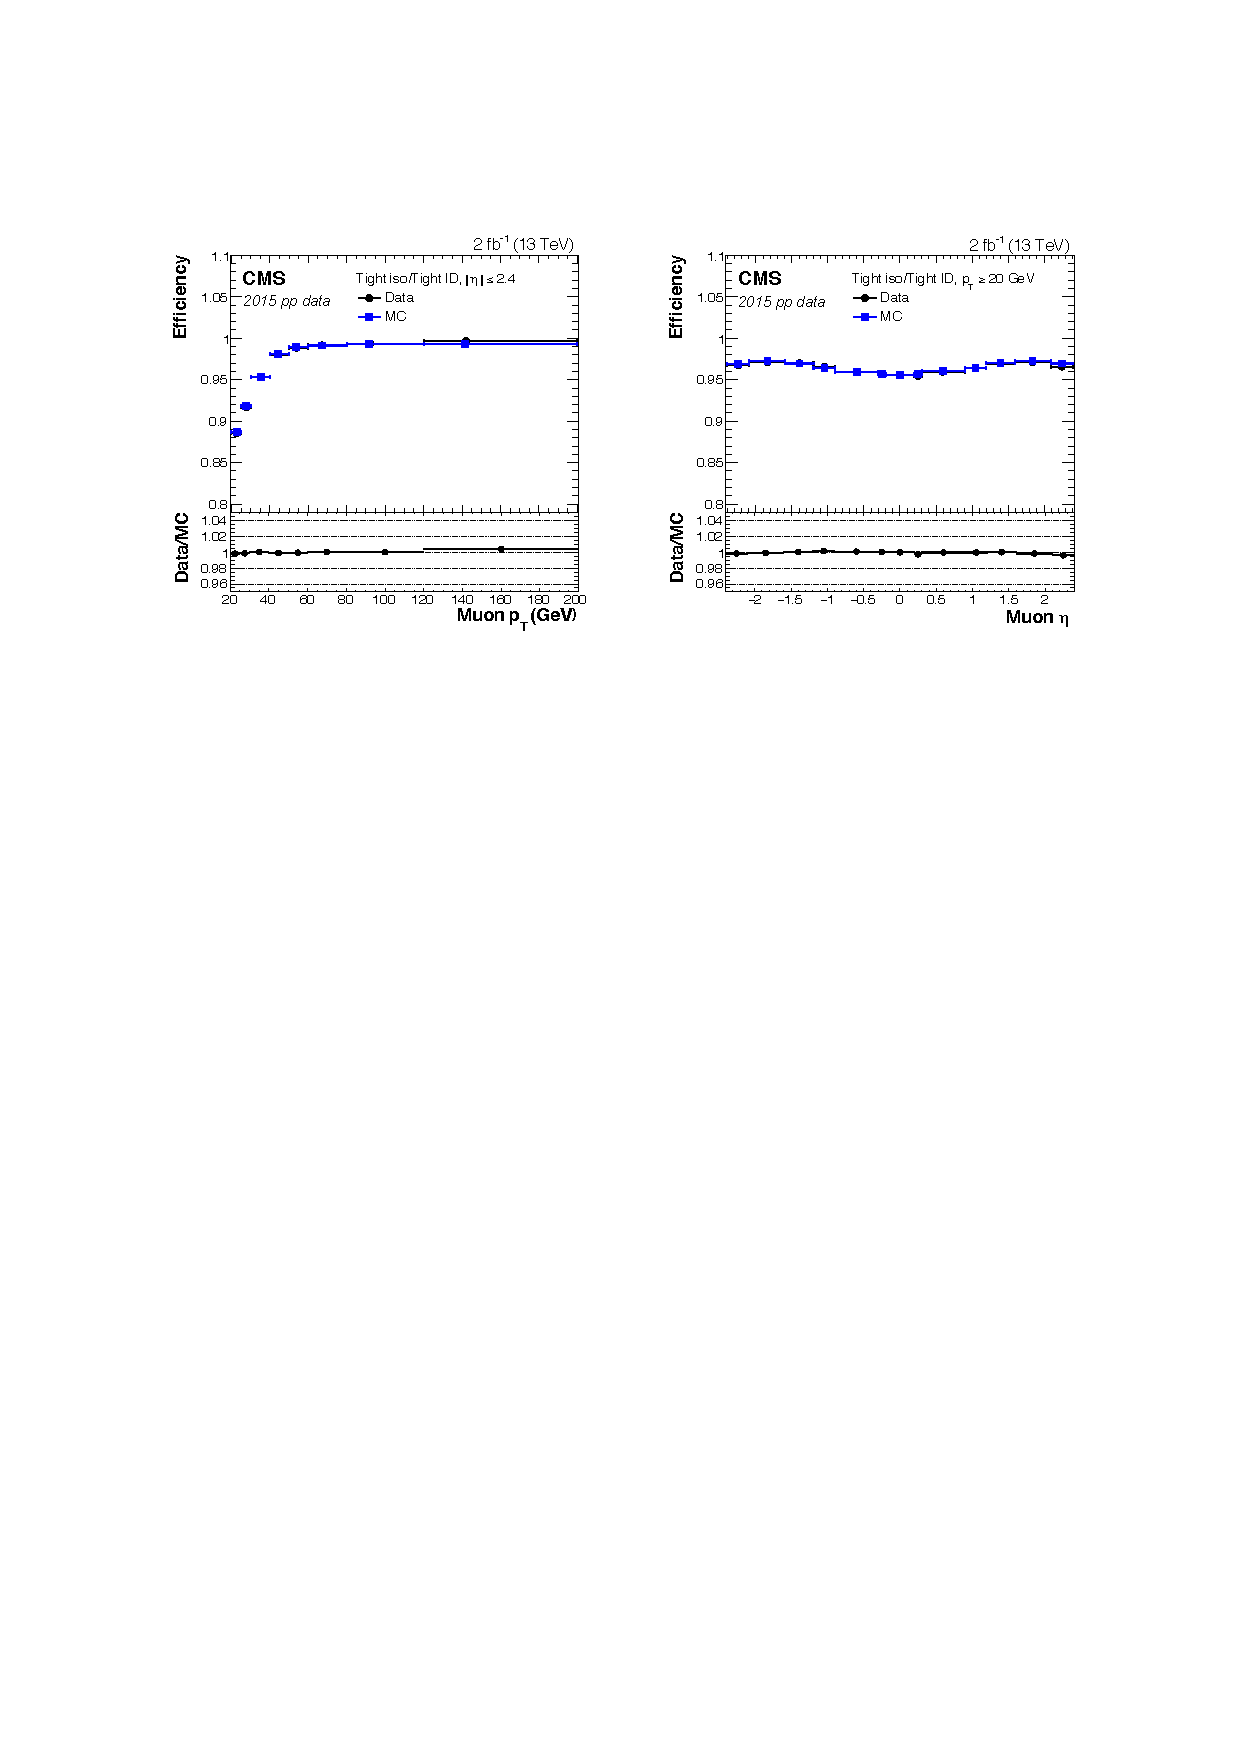
\includegraphics[width=\textwidth]{figure/reco_muon_eff.pdf}
    \caption[Tag-and-probe muon efficiency for the tight PF isolation working point on top of the tight ID]{
        Tag-and-probe efficiency for the tight PF isolation working point on top of the tight ID versus \PT for muons in the acceptance of the muon spectrometer (left), and versus $\eta$ for muons with $\PT > 20 \GeV$ (right), for 2015 data (circles), simulation (squares), and the ratio (bottom inset).
        The statistical uncertainties are smaller than the symbols used to display the measurements.
    }
    \label{fig:reco_muon_eff}
\end{figure}



    \section{Electron}
    Due to the small mass of electron, it tends to Bremsstrahlung radiation and energy decay in the tracker system.
Electrons are expected to generate a sequence of short tracks in the tracker system under the standard tracking algorithm.
The track segments, ECAL cluster for both the track-cluster linking, and photon tracks from Bremsstrahlung are masked from the ingredient list if the considered compatible to reconstruct into a particle-flow electron.
The following section will introudce the electron reconstruction and identification in the CMS experiment.

\subsection{Electron reconstruction}
The electron tracks give information for precise momentum measurement and to distinguish electrons from photons.
However, electrons can interact with inner tracker materials and ECAL crystals producing situations such as Bremsstrahlung and conversions, as shown in Fig.~\ref{fig:reco_el_track}.
The connection and integration process between these situations can be summarized in the following parts.

\begin{figure}\centering
    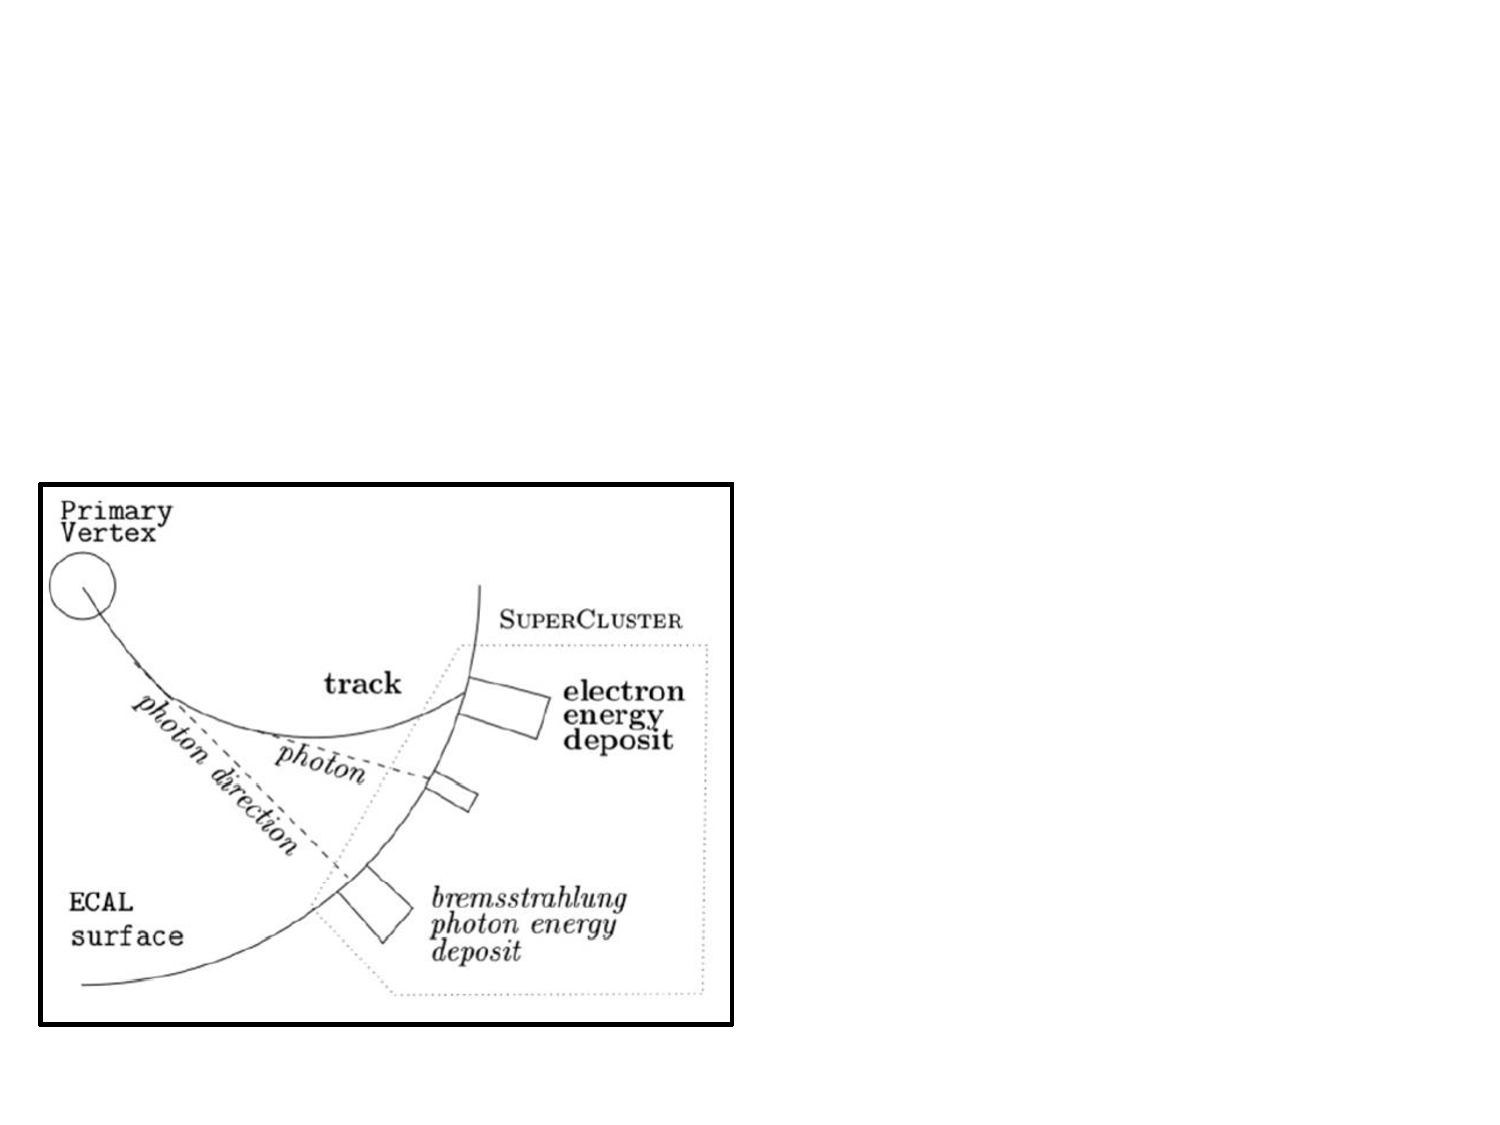
\includegraphics[width=0.75\textwidth]{figure/reco_el_track.pdf}
    \caption
    {
    Overview of an event with an electron including Bremsstrahlung tangent under the ECAL surface.
    }
    \label{fig:reco_el_track}
\end{figure}

The electron reconstruction begins with the EM supercluster reconstruction in the ECAL given by the PF cluster algorithm.
Since the Bremsstrahlung and photon conversion mainly happen with original electrons or photons from interaction points before hitting on the ECAL detector.
An ECAL cluster is not able to recover the energy of the original electrons.
The construction with supercluster, combining the associated ECAL clusters into a signal cluster, adopts a mustache algorithm to include the information from the ECAL and preshower detectors.
This algorithm starts from a seed cluster above a given threshold with additional clusters located in a mustache-like region in the $\eta-\phi$ plane (Fig.~\ref{fig:reco_beard}) to form a supercluster.
The clusters under the strong magnetic filed can then be collected under this design.

\begin{figure}\centering
    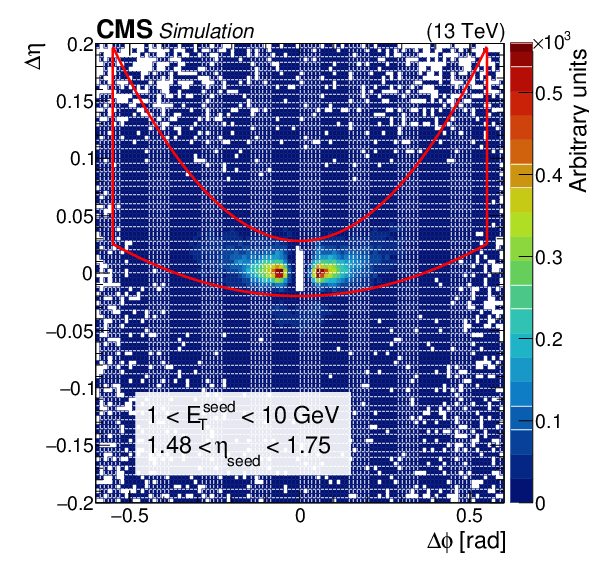
\includegraphics[width=0.55\textwidth]{figure/reco_beard.png}
    \caption[Distribution of $\Delta\eta$ versus $\Delta\phi$ for simulated electrons.]
    {
        Distribution of $\Delta\eta=\eta_{\mathrm{seed-cluster}}-\eta_{\mathrm{cluster}}$ versus $\Delta\phi = \phi_{\mathrm{seed-cluster}}  - \phi_{\mathrm{cluster}}$ for simulated electrons with $1 < \ET^{\mathrm{seed}} < 10 \GeV$ and $1.48 < \eta_{\mathrm{seed}} < 1.75$.
        The $z$-axis represents the occupancy of the number of PF clusters matched with the simulation (requiring to share at least $1\%$ of the simulated electron energy) around the seed. 
        The red line contains approximately the set of clusters selected by the mustache algorithm. 
        The white region at the center of the plot represents the $\eta-\phi$ footprint of the seed cluster.
    }
    \label{fig:reco_beard}
\end{figure}

The electrons are also reconstructed by track reconstruction in the CMS experiment.
To account for the electron energy loss from Bremsstrahlung at each layer of material, the electron tracks can be obtained after refitting the track segments with a Gaussian-sum filter (GSF) instead of the normal KF algorithm. 
The GSF track reconstruction begins with electron trajectory with either ECAL-driven seeding or tracker-driven seeding.
The ECAL-driven seeding chooses mustache clusters with $E_{\mathrm{SC,T}} > 4 \GeV$ and $H/E_{\mathrm{SC}} < 0.15$, where $E_{\mathrm{SC,T}}$ and $E_{\mathrm{SC}}$ are the transverse energy and total energy of the superclusters and $H$ indicates the HCAL tower energy deposited in $\Delta R < 0.15$ with the supercluster positions as the center.
Based on the assumption of the trajectory in a helix structure and no radiative emission, the trajectory is extrapolated to the collision vertex with the energy-weighted position, transverse energy and the magnetic filed in each selected supercluster.
The seed are considered as a electron track seed if the first two hits are matched to the extrapolated trajectory in the pixel layers or endcap tracker.
The tracker-driven seeding, in contrast, uses all inner tracks information.
The inner track seed is considered as a GSF track seed if a inner track is matched to an ECAL cluster with some track quality criteria.
Both of the seeds are then grouped together as the start point of the electron track reconstruction.
The GSF fit adopts a sum of multi-gaussian functions (as an approximation of the Bethe-Heitler formula) to estimate the parameters of the electron trajectories.

The superclusters and GSF tracks will be integrated together and the mustache superclusters will be associated with a GSF track once they are fully reconstructed.
The conversion vertexes and the associated tracks are made with information from the inner tracks, ECAL-seeded tracks and a kinematic vertex fitter.
The Bremsstrahlung photons are reconstructed by connecting the GSF tracks to the corresponding ECAL clusters via a Bremsstrahlung tangent, a extrapolated straight line.
The superclusters or the GSF tracks are connected with those conversion tracks and Bremsstrahlung tangents.
The ECAL clusters linked to both tracks are added to mustache superclusters to form refined superclusters.

Eventually, all the clusters and tracks are grouped together to form $\Pe/\gamma$ hypotheses.
The electron candidates, filter by loose criteria based on the BDT classifier to eliminate the fake ones from jet fragmentation and hadronization, is defined as an $\Pe/\gamma$ object.
The electron reconstruction efficiencies measured in 2017 data and in simulated DY samples are shown in Fig.~\ref{fig:reco_el_eff}.

\begin{figure}\centering
    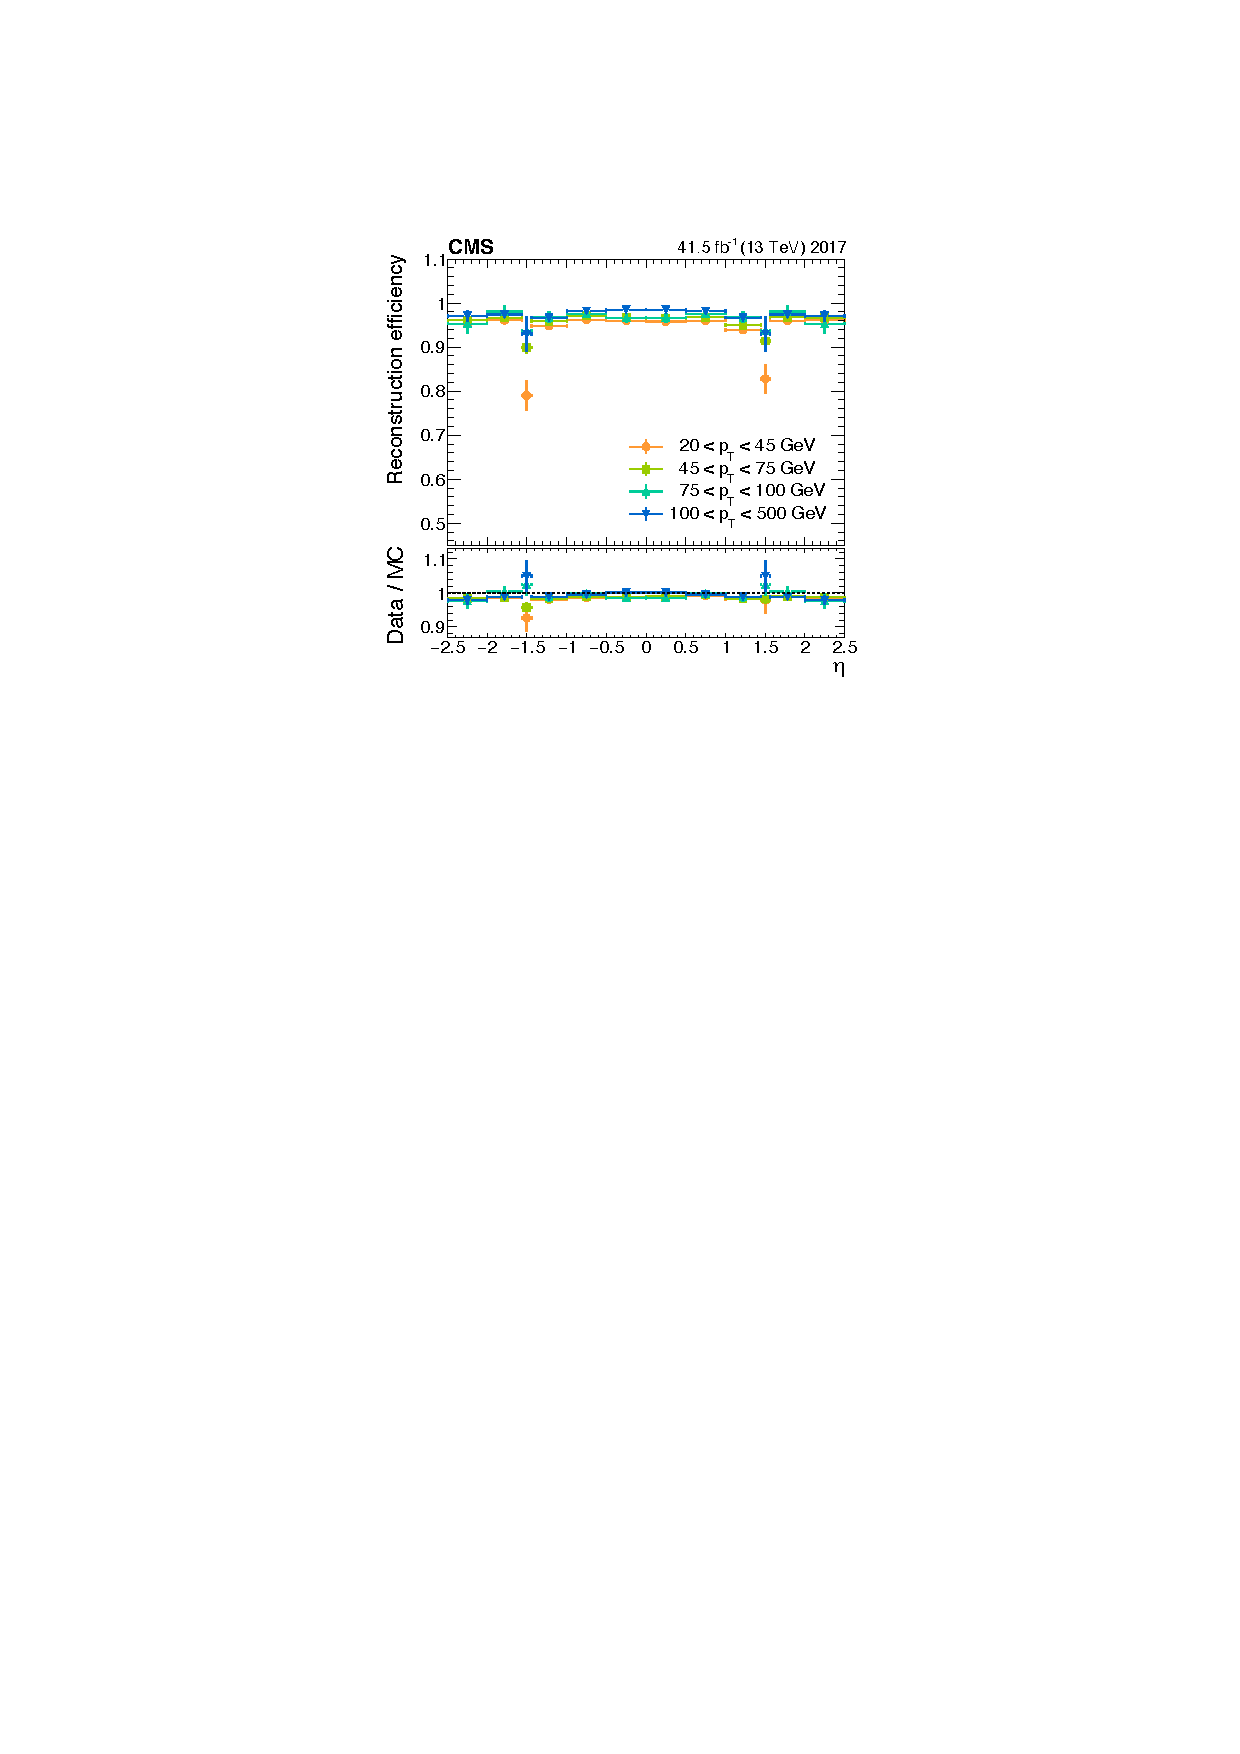
\includegraphics[width=0.55\textwidth]{figure/reco_el_eff.pdf}
    \caption[Electron reconstruction efficiency versus $\eta$ for the 2017 data.]
    {
        Electron reconstruction efficiency versus $\eta$ in data (upper panel) and data-to- simulation efficiency ratios (lower panel) for the 2017 data taking period. 
        The vertical bars on the markers represent the combined statistical and systematic uncertainties. 
        The region $1.44 < |\eta| < 1.57$ corresponds to the transition between the barrel and endcap regions of ECAL and is not considered in physics analyses.
    }
    \label{fig:reco_el_eff}
\end{figure}

\subsection{Electron identification and isolation}
The electron identification could be done by comparing the geometrical information, shape, and fitting properties between supercluster in the ECAL and track.
The isolation value is also defined similarly as Eq.~\ref{eq:reco_muon_iso}.

The $\Pe/\gamma$ physics object group defines the identification and isolation scheme with the following variables.
\begin{itemize}
    \item $\sigma_{|\eta|\eta}$: A spread of the ECAL supercluster in the $\eta$ direction.
        An electron from a hard process should have a narrow signature in the $\eta$ direction due to the occurrence of the bending radiation from electrons bending in the magnetic field.
    \item $|\Delta\eta|$ and $\Delta\Phi$: Geometric differences betwen the supercluster and the tracker.
    \item $H/E$: The ratio between the energy deposited in the HCAL and the ECAL in the super cluster region.
    \item $|\frac{1}{E}-\frac{1}{\rho}|$: Difference between the energy deposited in the supercluster and the track.
    \item $I_{\mathrm{PF,rel}}$ with EA: Isolation variable defined similarly to Eq.~\ref{eq:reco_muon_iso} with the effective areas.
    \item $d_{xy}$ and $d_z$: The impact parameters relative to a primary vertex.
    \item Missing hits in the tracker system.
    \item Whether the candidate passes the conversion veto cut.
\end{itemize}

The $\Pe/\gamma$ physics object group determines the exact cut values for each variable for different working points with different cut values for barrel and endcap electrons.
The cut values used in this analysis can be found in Tables~\ref{tab:reco_el_id_barrel} and~\ref{tab:reco_el_id_endcap}.


\begin{table}
    \caption[Electron identification and isolation cut values in barrel region.]
    {
        Electron identification and isolation cut values prescribed by the $\Pe/\gamma$ physics object group for barrel region $|\eta|<1.479$
    }
    \label{tab:reco_el_id_barrel}
    \centering\renewcommand\arraystretch{2.4}
    \resizebox{\textwidth}{!}{
        \begin{tabular}{|c|cccc|}
            \hline
            Variable & Veto & Loose & Medium & Tight \\
            \hline
            $\sigma_{|\eta|\eta} <$ & 0.0126 & 0.0112 & 0.0106 & 0.0104 \\
            $|\Delta\eta| <$                         & 0.00463 & 0.00377 & 0.0032 & 0.00255 \\
            $\Delta\Phi <$                          & 0.0148 &    0.0884 & 0.0547 & 0.022 \\
            $H/E < $  & $0.05+1.16/E_{\mathrm{SC}}+0.0324 \times \rho/E_{\mathrm{SC}}$ & $0.05+1.16/E_{\mathrm{SC}}+0.0324 \times \rho/E_{\mathrm{SC}}$ & $0.046+1.16/E_{\mathrm{SC}}+0.0324 \times \rho/E_{\mathrm{SC}}$ & $0.026+1.16/E_{\mathrm{SC}}+0.0324 \times \rho/E_{\mathrm{SC}}$ \\
            $I_{\mathrm{PF,rel}}$ with EA $<$ & $0.198+0.506/\PT$ & $0.112+0.506/\PT$ & $0.0478+0.506/\PT$ & $0.0287+0.506/\PT$ \\
            $1/E - 1/\rho <$ & 0.209 & 0.193 & 0.184 & 0.159 \\
            Missing inner hits $\leq$ & 2 & 1 & 1 & 1\\
            Pass conversion veto & Y & Y & Y & Y\\
            \hline
        \end{tabular}
    }
\end{table}

\begin{table}
    \caption[Electron identification and isolation cut values in endcap region.]
    {
        Electron identification and isolation cut values prescribed by the $\Pe/\gamma$ physics object group for endcap region $|\eta|>1.479$
    }
    \label{tab:reco_el_id_endcap}
    \centering\renewcommand\arraystretch{2.4}
    \resizebox{\textwidth}{!}{
        \begin{tabular}{|c|cccc|}
            \hline
            Variable & Veto & Loose & Medium & Tight \\
            \hline
            $\sigma_{|\eta|\eta} <$ & 0.0457 & 0.0425 & 0.0387 & 0.0353 \\
            $|\Delta\eta| <$        & 0.00814	& 0.00674	& 0.00632	& 0.00501\\
            $\Delta\Phi <$          & 0.19	& 0.169	& 0.0394 & 0.0236\\
            $H/E < $  & $0.05+2.54/E_{\mathrm{SC}}+0.183 \times \rho/E_{\mathrm{SC}}$ & $0.0441+2.54/E_{\mathrm{SC}}+0.0183 \times \rho/E_{\mathrm{SC}}$ & $0.0275+2.52/E_{\mathrm{SC}}+0.0183 \times \rho/E_{\mathrm{SC}}$ & $0.0188+2.06/E_{\mathrm{SC}}+0.183 \times \rho/E_{\mathrm{SC}}$ \\
            $I_{\mathrm{PF,rel}}$ with EA $<$ & $0.203+0.963/\PT$ & $0.108+0.963/\PT$ & $0.0658+0.963/\PT$ & $0.0445+0.963/\PT$ \\
            $1/E - 1/\rho <$ & 0.132 & 0.111 & 0.0721 & 0.0197 \\
            Missing inner hits $\leq$ & 3 & 1 & 1 & 1\\
            Pass conversion veto & Y & Y & Y & Y\\
            \hline
        \end{tabular}
    }
\end{table}

    \section{Jet}
    In this analysis, quarks or gluons can be produced via the strong interaction from a hard scattering process.
Due to QCD colr confinement, these strong interaction particles can emit soft gluons producing quark and anti-quark pairs or gluons, ending up with colorless particles, hadrons.
Some unstable hadrons then decay immediately to stable particles such as other hadrons, photons, or leptons, forming a shower of particles called jets.
It is common to cluster these showers as a single object to represent the underlying parton.

\subsection{Jet reconstruction}
Jets are reconstructed by clustering showers of the particle-flow candidates.
The clustering algorithm compares two different distance measures $d_i$ and $d_{ij}$ and update the jet candidates to complete the process.
The $d_i$ is the distance between the original beam and the particle $i$ from an existing list of particles.
The $d_{ij}$ is the distance between the particle $i$ and a half constructed pseudo-jet.
The two distance measures are given as
\begin{linenomath}\begin{equation}\begin{aligned}\label{eq:reco_anti_kt}
    d_{i}  &= p_{\mathrm{T},i}^{2p}  \\
    d_{ij} &= min[p_{\mathrm{T},i}^{2p}, p_{\mathrm{T},j}^{2p}] \times \frac{\Delta^2_{ij}}{R^2}
\end{aligned}\end{equation}\end{linenomath}
where $p_{\mathrm{T},i}$ is the transverse momentum of particle $i$, $p_{\mathrm{T},j}$ is the transverse momentum of the pseudo-jet, $\Delta_{ij}$ is the angular separation of the particle $i$ and pseudo-jet $j$, $R$ is some angular size parameter defined by user, and $p$ is also a factor that is defined by the user.
The particle $i$ with $d_{ij}$ smaller than $d_i$ is considered close to the pseudo-jet $j$ and thus is merged into the pseudo-jet object.
The kinematics of the pseudo-jet object are then re-computed, and the particle $i$ is removed from the original particle list.
This process is complete when no particle can be added to the pseudo-jet, and a new pseudo-jet is created with the largest \PT particle in the remaining particle list.

This clustering algorithm is commonly used in the CMS experiment with the value of $p=-1$, and thus referred to the anti-$K_{\mathrm{T}}$ algorithm.
This algorithm allows the jet clustering to be less sensitive to the existence of particles originating from soft processes and thus making itself less sensitive to the high pileup situation, as shown in Fig.~\ref{fig:reco_antikt.png}.
The size parameter used in this analysis is $R=0.4$.
\begin{figure}\centering
    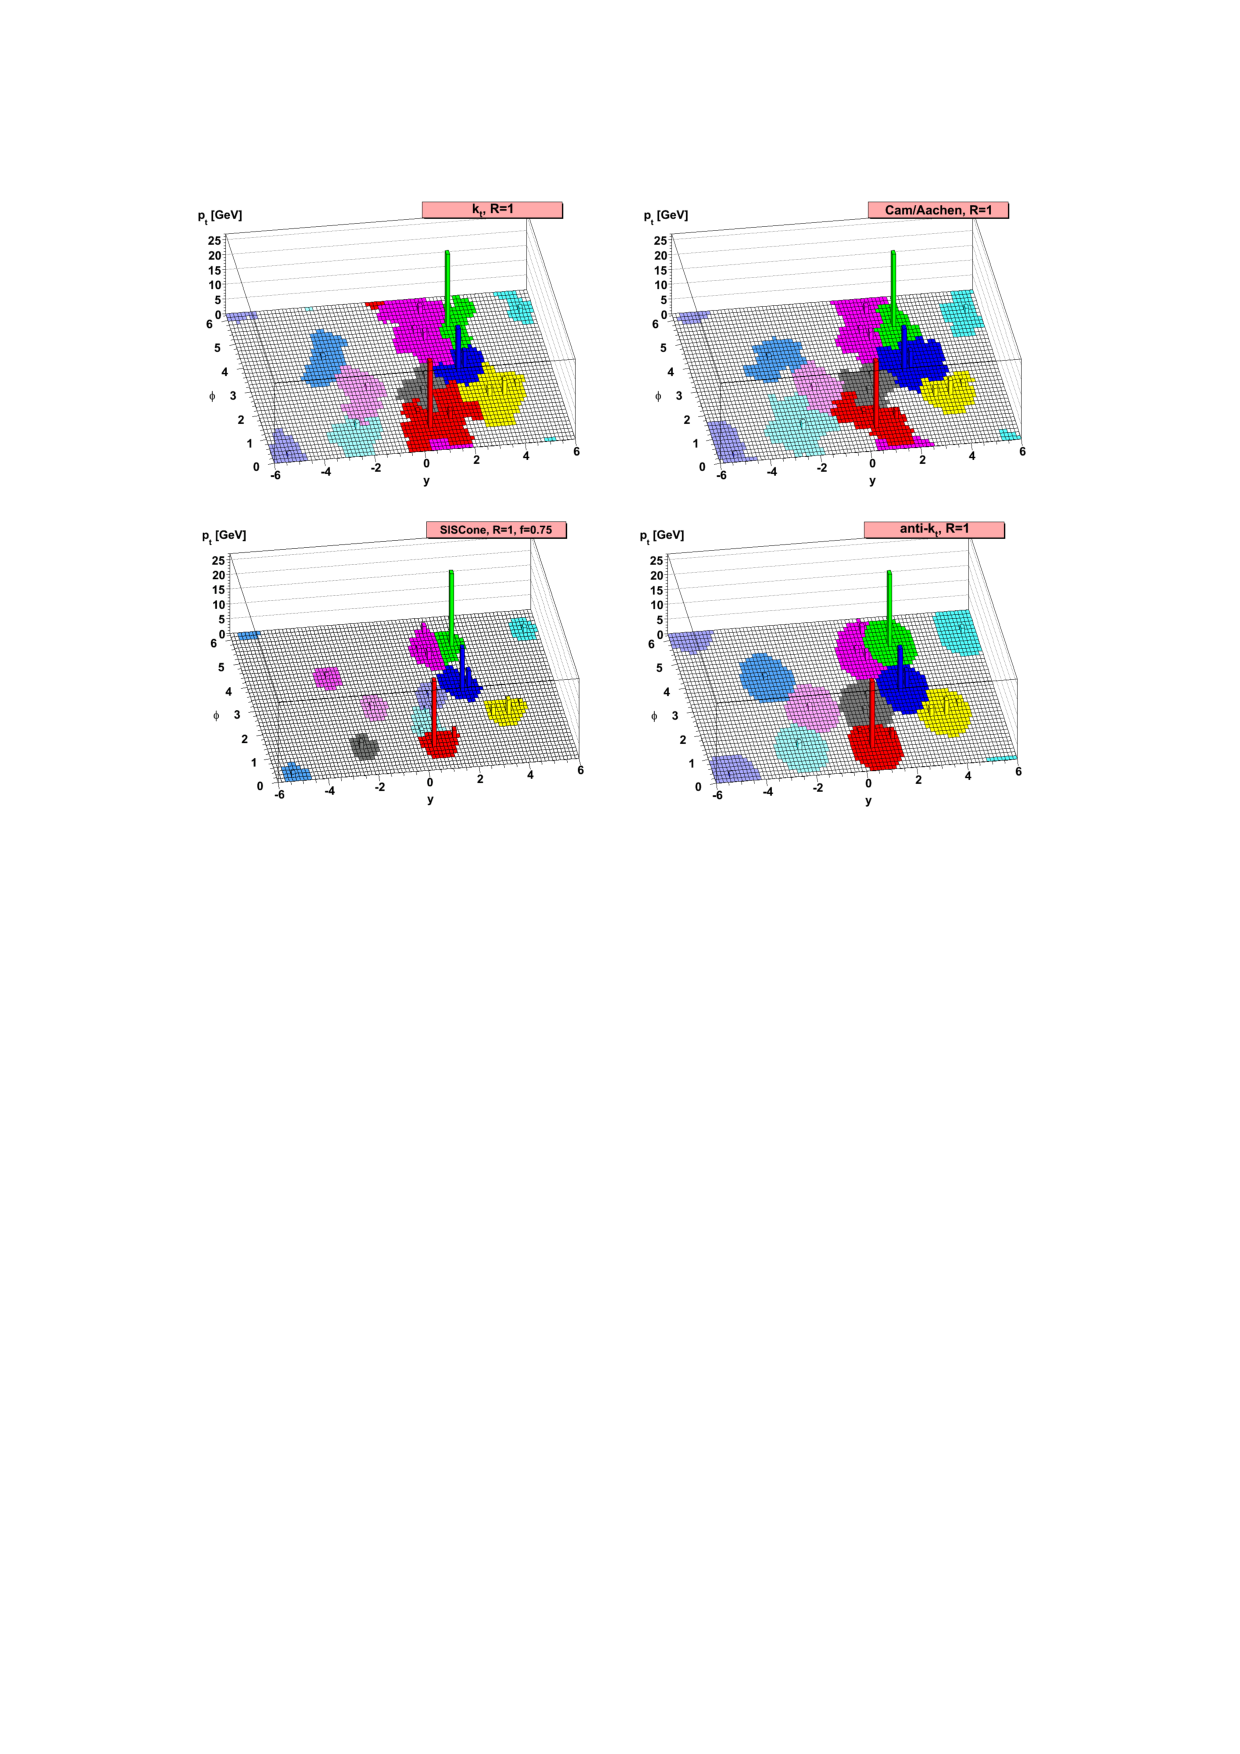
\includegraphics[width=0.7\textwidth]{figure/reco_antikt.pdf}
    \caption[Comparison of the jet clustering algorithm.]
    {
        Comparison of the jet clustering algorithm with randomly injected ghost particles, all using a radius parameter of $R=1$.
        The cluster boundaries in anti-$K_{\mathrm{T}}$ algorithm more determined by the hard center of the jets.
    }
    \label{fig:reco_antikt.png}
\end{figure}

\subsection{Jet corrections}
The kinematics of underlying partons from the strong interaction in the hard processes should be reflected to the jets.
This can be achieved by applying calibration factors obtained from detector responses and simulation assisted corrections to the jet kinematics (raw sum of all constituent particles).

The contribution from the pileup effect, leading to incorrect energy reconstruction of jets with charged particles candidates from pileup vertices, should be removed.
This process is called the charged hadron subtraction (CHS).

The contribution of neutral particles from pileup interactions, which can be estimated from the averaged energy area density $\rho_E$ for the event and the jet area, should also be removed.
This process is called the L1 pileup correction.

Further corrections such as L2L3 truth corrections should also be considered.
Those corrections are computed by directly comparing the true clustering momentum obtained from the constituent particles in simulation with the reconstruction momentum from the clustering algorithm.

The truth corrections can be further developed as the L2L3 residual corrections which are typically small.
To account for the differences in different detector responses in data and simulation, well-known jet emitting processes, such as the QCD multi-jet events can be studied.

\subsection{Jet identification}
Jet identification schemes are designed to reject noise such as jets forming around a lepton with soft radiation particle under the jet clustering algorithm.
It requires the reconstructed jet should be from good composition of various particle flavors (Fig.~\ref{fig:reco_jet}) to help identify jets originating from QCD particles.
\begin{figure}\centering
    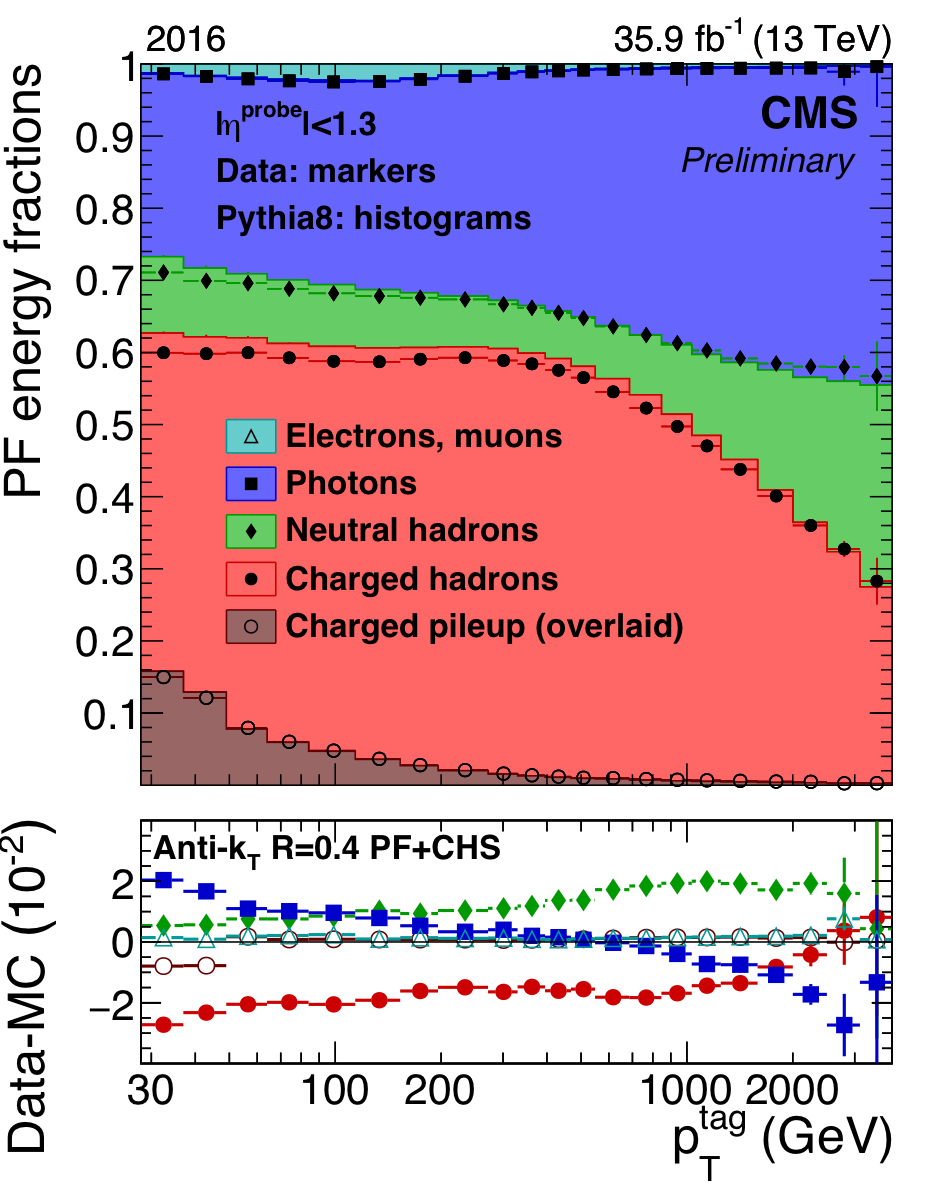
\includegraphics[width=0.3\textwidth]{figure/reco_jet16.png}
    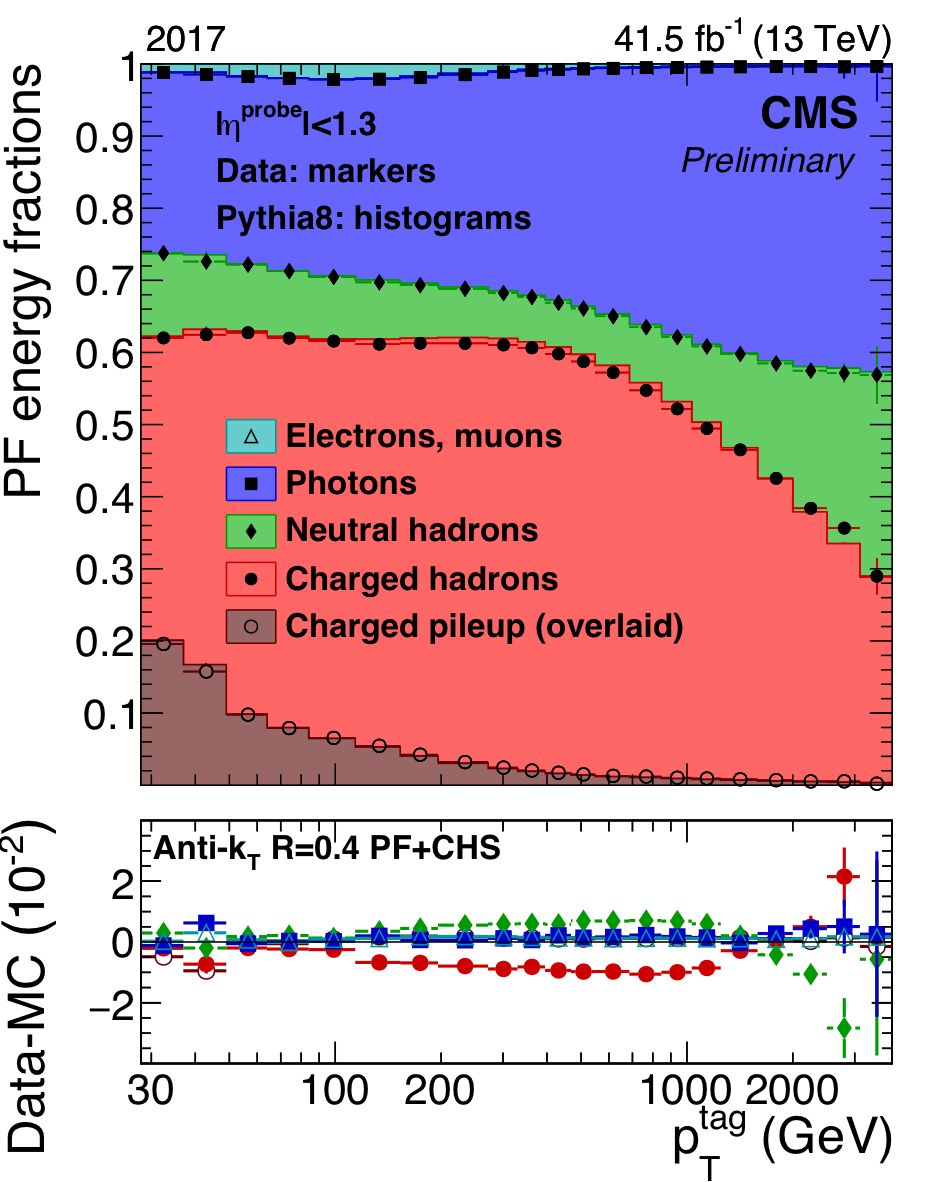
\includegraphics[width=0.3\textwidth]{figure/reco_jet17.png}
    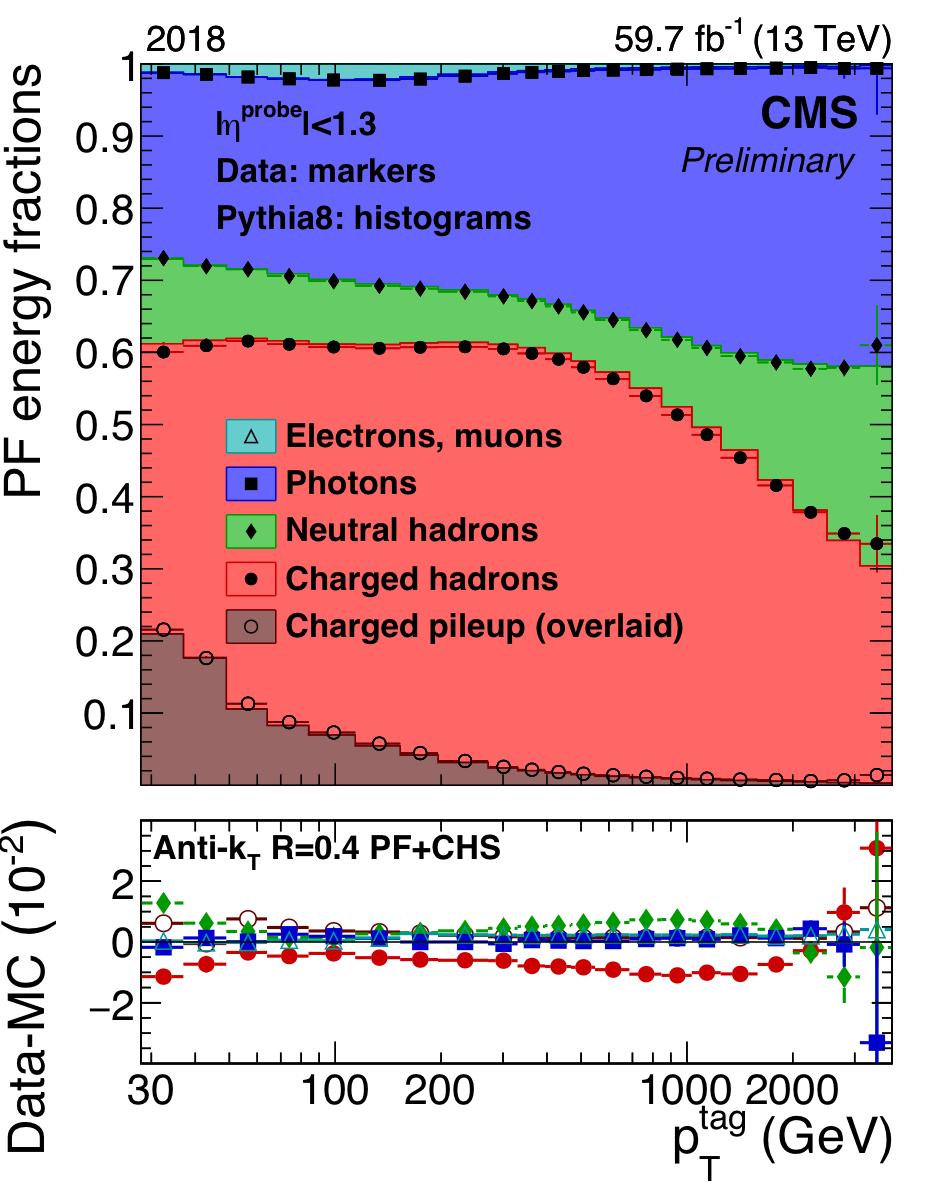
\includegraphics[width=0.3\textwidth]{figure/reco_jet18.png}
    \caption[Jet energy composition of various particle-flow candidates.]
    {
        Jet energy composition of various particle-flow candidates.
        Jets are clustered using the anti-$K_{\mathrm{T}}$ algorithm with size parameter $R=0.4$ during RunII.
    }
    \label{fig:reco_jet}
\end{figure}

The cuts used for jet identification at a loose working point for 2016 samples and a tight working point for 2017 and 2018 samples, both at around $99\%$ efficiency of selecting genuine jets.
All the jets are required to be within $|\eta|<2.4$ region and the detailed cut value in this analysis can be found in Table~\ref{tab:reco_jetid}.
\begin{table}
    \caption{Criteria of jet identification at different working points.}
    \label{tab:reco_jetid}
    \centering
    \begin{tabular}{ccc}
        \hline
        Variable & Loose & Tight\\
        \hline
        Neutral hadron energy fraction $<$ & 0.99 & 0.90\\
        Neutral EM energy fraction $<$ & 0.99 & 0.90\\
        Number of constituents $>$ 1 & 1\\
        Charged hadron energy fraction $>$ & 0 & 0\\
        Charged EM energy fraction $<$ & 0.99 & -\\ 
        Charged multiplicity $>$ & 0 & 0\\
        \hline
    \end{tabular}
\end{table}

\subsection{Jet flavor tagging}
The underlying parton flavor could be inferred from the constituents of the jets, however, not 100$\%$ correct in data.
Jets passing some threshold of the discriminator are typically called flavor tagged jets.

Jets with the underlying \PQb quark have relatively longer lifetime ($\mathcal{O}(\ten{-12})$ s) since the \PQb quark decays are suppressed by the elements $V_{\PQu\PQb}$ and $V_{\PQc\PQb}$ in the CKM matrix.
These b hadrons can propagate a longer distance from a few mm to one cm, and thus jets originating from \PQb quarks have signatures that is more easily identified.
The flight distance can be calculated with a \PQb hadron with mass $m$ on the order of $\approx 5\GeV$, energy $E$ on the order of $\approx 50 \GeV$, and an average lifetime $\tau$ on the order of $\approx \ten{-12}$ sec as 
\begin{linenomath}\begin{equation}\begin{aligned}\label{eq:reco_bjet}
    d_{\mathrm{flight}} &\approx v\tau\sqrt{1+(\frac{p}{mc})^2} \approx c\tau\frac{E}{mc^2} \\
                        &\approx 10^{-2} \mathrm{m}
\end{aligned}\end{equation}\end{linenomath}
This displacement creates a secondary vertex (SV) with significant transverse distance from the primary vertex illustrated in Fig.~\ref{fig:reco_bjet}.
\begin{figure}\centering
    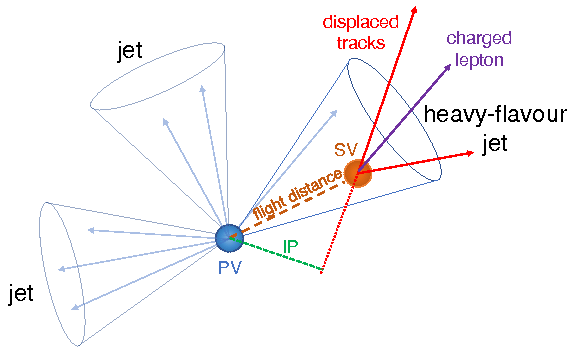
\includegraphics[width=0.7\textwidth]{figure/reco_bjet.png}
    \caption[Illustration of variable useful for \PQb tagging algorithm.]
    {
        Illustration of a heavy-flavour jet with a secondary vertex (SV) from the decay of a \PQb or \PQc hadron resulting in charged-particle tracks (including possibly a soft lepton) that are displaced with respect to the primary interaction vertex (PV), and hence with a large impact parameter (IP) value. 
    }
    \label{fig:reco_bjet}
\end{figure}

The features above can be used to compute a ML-based combined secondary vertex (CSV) discriminating factor.
It has been widely used in the CMS experiment for the \PQb jet identification during RunI, and has been improved with a deep neural network (DNN) during RunII to cope with higher pilup environment.
The improved CSV  discriminator, called DeepCSV, uses information such as the impact parameters with respect to the primary vertices and the mass of the secondary vertex.
The \PQb tagging efficiency and misidentified efficiency under DeepCSV discriminator are shown in Fig.~\ref{fig:reco_beff} and Fig.~\ref{fig:reco_misb}, respectively.

\begin{figure}\centering
    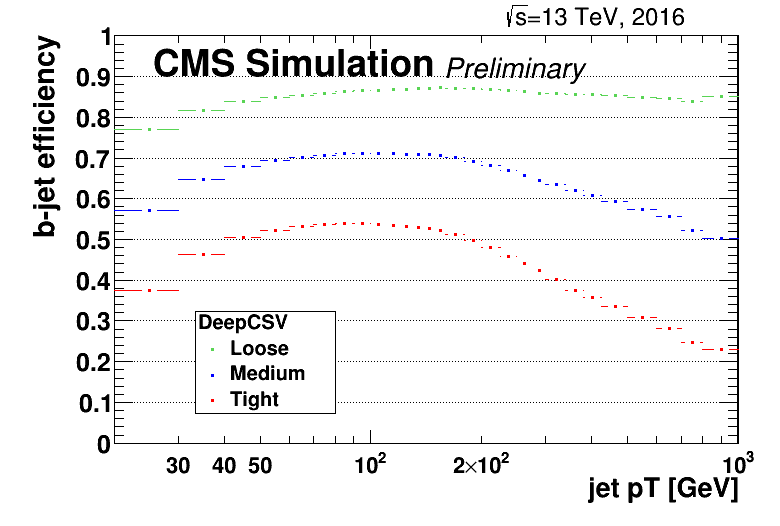
\includegraphics[width=0.7\textwidth]{figure/reco_beff.png}
    \caption
    {
        The efficiency of \PQb tagging as a function of the jet transverse momentum for the DeepCSV algorithms. 
    }
    \label{fig:reco_beff}
\end{figure}

\begin{figure}\centering
    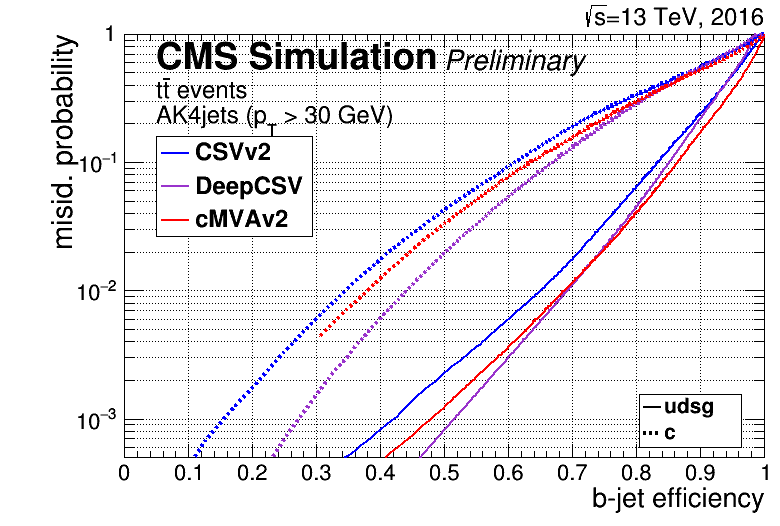
\includegraphics[width=0.7\textwidth]{figure/reco_misb.png}
    \caption[\PQb misidentified efficiency as a function of the \PQb tagging efficiency.]
    {
        Performance of the \PQb jet identification efficiency algorithms demonstrating the probability for non-b jets to be misidentified as \PQb jet as a function of the efficiency to correctly identify \PQb jets. 
        The curves are obtained on simulated \ttbar events using jets within tracker acceptance with $\PT>30 \GeV$, \PQb jets from gluon splitting to a pair of \PQb quarks are considered as \PQb jets.
    }
    \label{fig:reco_misb}
\end{figure}

\chapter{Data and simulated samples}
    \section{Data samples}
    This study involves data from \pp collisions at \newTeV collected with the CMS detector in 2016--2018, corresponding to an integrated luminosity of 138\fbinv with an overall luminosity uncertainty of 1.6\%~\cite{CMS:lumi2016, CMS:lumi2017, CMS:lumi2018}.
Since the final state must include one isolated muon or electron, only the SingleMuon and SingleElectron data streams, where at least one muon or electron trigger was fired, are taken into consideration.
A summary of all the used datasets and the corresponding intergrated luminosity can be found in Table~\ref{tab:data_list}.

\begin{table}
    \caption{List of \newTeV collision data taken during RunII used in this analysis.}
    \label{tab:data_list}
    \centering\renewcommand\arraystretch{1.4}
    \begin{tabular}{cc}
        \hline 
        2016 Dataset & $\mathcal{L}$($fb^{-1}$) \\
        \hline
        /SingleElectron/Run2016B-17Jul2018\_ver2-v1/MINIAOD  & 5.75 \\
        /SingleElectron/Run2016C-17Jul2018-v1/MINIAOD       & 2.57 \\
        /SingleElectron/Run2016D-17Jul2018-v1/MINIAOD       & 4.24 \\
        /SingleElectron/Run2016E-17Jul2018-v1/MINIAOD       & 4.03 \\
        /SingleElectron/Run2016F-17Jul2018-v1/MINIAOD       & 3.10 \\
        /SingleElectron/Run2016G-17Jul2018-v1/MINIAOD       & 7.58 \\
        /SingleElectron/Run2016H-17Jul2018-v1/MINIAOD       & 8.65 \\
        \hline
        /SingleMuon/Run2016B-17Jul2018\_ver2-v1/MINIAOD      & 5.75 \\
        /SingleMuon/Run2016C-17Jul2018-v1/MINIAOD           & 2.57 \\
        /SingleMuon/Run2016D-17Jul2018-v1/MINIAOD           & 4.24 \\
        /SingleMuon/Run2016E-17Jul2018-v1/MINIAOD           & 4.03 \\
        /SingleMuon/Run2016F-17Jul2018-v1/MINIAOD           & 3.10 \\
        /SingleMuon/Run2016G-17Jul2018-v1/MINIAOD           & 7.58 \\
        /SingleMuon/Run2016H-17Jul2018-v1/MINIAOD           & 8.65 \\
        \hline
        2017 Dataset & $\mathcal{L}$($fb^{-1}$) \\
        \hline 
        /SingleElectron/Run2017B-31Mar2018-v1/MINIAOD       & 4.79 \\
        /SingleElectron/Run2017C-31Mar2018-v1/MINIAOD       & 9.63 \\
        /SingleElectron/Run2017D-31Mar2018-v1/MINIAOD       & 4.25 \\
        /SingleElectron/Run2017E-31Mar2018-v1/MINIAOD       & 9.31 \\
        /SingleElectron/Run2017F-31Mar2018-v1/MINIAOD       & 13.54 \\
        \hline
        /SingleMuon/Run2017B-31Mar2018-v1/MINIAOD           & 4.79 \\
        /SingleMuon/Run2017C-31Mar2018-v1/MINIAOD           & 9.63 \\
        /SingleMuon/Run2017D-31Mar2018-v1/MINIAOD           & 4.25 \\
        /SingleMuon/Run2017E-31Mar2018-v1/MINIAOD           & 9.31 \\
        /SingleMuon/Run2017F-31Mar2018-v1/MINIAOD           & 13.54 \\
        \hline
        2018 Dataset & $\mathcal{L}$($fb^{-1}$) \\
        \hline 
        /EGamma/Run2018A-17Sep2018-v2/MINIAOD               & 14.03 \\
        /EGamma/Run2018B-17Sep2018-v1/MINIAOD               & 7.07 \\
        /EGamma/Run2018C-17Sep2018-v1/MINIAOD               & 6.90 \\
        /EGamma/Run2018D-PromptReco-v2/MINIAOD              & 31.75 \\
        \hline
        /SingleMuon/Run2018A-17Sep2018-v2/MINIAOD           & 14.03 \\
        /SingleMuon/Run2018B-17Sep2018-v1/MINIAOD           & 7.07 \\
        /SingleMuon/Run2018C-17Sep2018-v1/MINIAOD           & 6.90 \\
        /SingleMuon/Run2018D-PromptReco-v2/MINIAOD          & 31.75 \\
        \hline
    \end{tabular}
\end{table}

    \section{Simulated samples}
    The \ttbar production events are simulated using Monte Carlo (MC) programs.
The \ttbar is simulated using quantum chromodynamics (QCD) at next-to-leading-order (NLO) precision through the matrix element (ME) in the \POWHEG 2.0 event generator~\cite{Sim:powheg1, Sim:powheg2, Sim:powheg3, Sim:powheg4}.
The value of the top quark mass (\Mt) is set to 172.5\GeV.
The \POWHEG output is combined with the parton shower (PS) simulation of \PYTHIA 8.205~\cite{Sim:pythia2}, with the underlying-event (UE) tune CP5~\cite{Sim:CP5}.
The parton distribution functions (PDFs) NNPDF 3.1~\cite{Sim:NNPDF3.1} at next-to-NLO order (NNLO) are used to model the data.
Samples of \ttbar with different values of CEDM are simulated with the \MADGRAPH generator~\cite{Sim:madgraph} at leading-order (LO) precision interfaced with \PYTHIA.
These samples are used as a cross-check of the model dependency of each CP observable.

Several backgrounds are considered with single top quark production being the leading contribution.
The single top quark production is simulated at NLO using \MADGRAPH 2.4.2 with the FxFx matching scheme~\cite{Sim:FXFX} for $s$-channel production and \POWHEG for $t$-channel and $\PQt\PW$ production.
All samples are interfaced with \PYTHIA through the UE tune CUETP8M1~\cite{Sim:CUETP8M1} for $t$-channel production for the 2016 data and CP5 for the rest.
Diboson ($\PV\PV$), \Wjets, Drell--Yan (DY), and QCD multijet productions are simulated at LO using the \MADGRAPH 2.4.4 generator.
They are then interfaced with \PYTHIA using the MLM matching scheme~\cite{Sim:MLMmatching}.
Events coming from the decay of \ttbar into either dilepton+jets or hadronic multijets can be incorrectly included in the signal event sample due to particle misidentification.
They are considered as a background.
The background from \PW boson events with heavy-flavor quarks (\WHF), which is not a large background, is important during the estimation of the systematic uncertainties, and will be discussed in detail in Section~\ref{sec:uncertainty}.
List of all the simulated samples with various hard process used in this analysis can be found in Tables~\ref{tab:mc_list_16},~\ref{tab:mc_list_17}, and~\ref{tab:mc_list_18}.

The simulation of the experimental apparatus is based on \GEANTfour~\cite{Sim:geant4}.
To model the effect of additional \pp interactions within the same or nearby bunch crossings (pileup), simulated minimum-bias interactions are included in the simulated samples~\cite{Sim:pileup}.
The number of pileup interactions in the simulation is reweighted to match the distribution in data.
\begin{table}[H]
    \caption{List of 2016 simulated samples used in this analysis}
    \label{tab:mc_list_16}
    \centering
    \resizebox{\textwidth}{!}{
        \begin{tabular}{|l|cc|c|}
    \hline
    Process & Cross section ($pb$) & K Factor\\
    \hline
    \multicolumn{3}{|c|}{Signal}\\
    \hline
    TTToSemiLeptonic\_TuneCP5\_PSweights\_13TeV-powheg-pythia8                                   &  $831.76 * 0.44113$(NNLO)       & 1 \\
    TTTo2L2Nu\_TuneCP5\_PSweights\_13TeV-powheg-pythia8                                          &  $831.76 * 0.10706$(NNLO)       & 1 \\
    TTToHadronic\_TuneCP5\_PSweights\_13TeV-powheg-pythia8                                       &  $831.76 * 0.45441$(NNLO)       & 1 \\
    \hline
    \multicolumn{3}{|c|}{Background}\\
    \hline 
    QCD\_HT100to200\_TuneCUETP8M1\_13TeV-madgraphMLM-pythia8                                     &     $27990000$(LO)              & 1 \\
    QCD\_HT200to300\_TuneCUETP8M1\_13TeV-madgraphMLM-pythia8                                     &     $1712000$(LO)               & 1 \\
    QCD\_HT300to500\_TuneCUETP8M1\_13TeV-madgraphMLM-pythia8                                     &     $347700$(LO)                & 1 \\
    QCD\_HT500to700\_TuneCUETP8M1\_13TeV-madgraphMLM-pythia8                                     &     $32100$(LO)                 & 1 \\
    QCD\_HT700to1000\_TuneCUETP8M1\_13TeV-madgraphMLM-pythia8                                    &     $6831$(LO)                  & 1 \\
    QCD\_HT1000to1500\_TuneCUETP8M1\_13TeV-madgraphMLM-pythia8                                   &     $1207$(LO)                  & 1 \\
    QCD\_HT1500to2000\_TuneCUETP8M1\_13TeV-madgraphMLM-pythia8                                   &     $119.9$(LO)                 & 1 \\
    QCD\_HT2000toInf\_TuneCUETP8M1\_13TeV-madgraphMLM-pythia8                                    &     $25.2$(LO)                  & 1  \\
    \hline
    WW\_TuneCUETP8M1\_13TeV-pythia8                                                              &   $118.7$(NLO)                  &1\\
    ZZ\_TuneCUETP8M1\_13TeV-pythia8                                                              &   $16.5$(NLO)                   &   1  \\      
    WZ\_TuneCUETP8M1\_13TeV-pythia8                                                              &   $47.1$(NLO)                   &   1  \\                
    ST\_s-channel\_4f\_leptonDecays\_TuneCP5\_PSweights\_13TeV-amcatnlo-pythia8                  &   $3.36$(NLO)                     &   1    \\
    ST\_t-channel\_top\_4f\_inclusiveDecays\_13TeV-powhegV2-madspin-pythia8\_TuneCUETP8M1         &   $136.02$(NLO)                   &   1    \\
    ST\_t-channel\_antitop\_4f\_InclusiveDecays\_TuneCP5\_PSweights\_13TeV-powheg-pythia8        &   $80.95$(NLO)                    &   1    \\
    ST\_tW\_top\_5f\_inclusiveDecays\_TuneCP5\_PSweights\_13TeV-powheg-pythia8                   &   $35.6$(NLO)                     &   1    \\
    ST\_tW\_antitop\_5f\_inclusiveDecays\_TuneCP5\_PSweights\_13TeV-powheg-pythia8               &   $35.6$(NLO)                     &   1    \\
    \hline
    WJetsToLNu\_HT-100To200\_TuneCUETP8M1\_13TeV-madgraphMLM-pythia8                             &     $1345.7$(LO)                & 1.21  \\
    WJetsToLNu\_HT-200To400\_TuneCUETP8M1\_13TeV-madgraphMLM-pythia8                             &     $359.7$(LO)                 & 1.21  \\
    WJetsToLNu\_HT-400To600\_TuneCUETP8M1\_13TeV-madgraphMLM-pythia8                             &      $48.9$(LO)                  & 1.21  \\
    WJetsToLNu\_HT-600To800\_TuneCUETP8M1\_13TeV-madgraphMLM-pythia8                             &      $12.1$(LO)                  & 1.21  \\
    WJetsToLNu\_HT-800To1200\_TuneCUETP8M1\_13TeV-madgraphMLM-pythia8                            &     $5.5$(LO)                   & 1.21  \\
    WJetsToLNu\_HT-1200To2500\_TuneCUETP8M1\_13TeV-madgraphMLM-pythia8                           &     $1.3$(LO)                   & 1.21  \\
    WJetsToLNu\_HT-2500ToInf\_TuneCUETP8M1\_13TeV-madgraphMLM-pythia8                            &     $3.2\times 10^{-2}$(LO)     & 1.21  \\
    DYJetsToLL\_M-50\_HT-70to100\_TuneCUETP8M1\_13TeV-madgraphMLM-pythia8             &     $169.9$(LO)                 & 1.23  \\
    DYJetsToLL\_M-50\_HT-100to200\_TuneCUETP8M1\_13TeV-madgraphMLM-pythia8            &     $147.4$(LO)                 & 1.23  \\
    DYJetsToLL\_M-50\_HT-200to400\_TuneCUETP8M1\_13TeV-madgraphMLM-pythia8            &     $41.0$(LO)                  & 1.23  \\
    DYJetsToLL\_M-50\_HT-400to600\_TuneCUETP8M1\_13TeV-madgraphMLM-pythia8            &     $5.7$(LO)                   & 1.23  \\
    DYJetsToLL\_M-50\_HT-600to800\_TuneCUETP8M1\_13TeV-madgraphMLM-pythia8            &     $1.4$(LO)                   & 1.23  \\
    DYJetsToLL\_M-50\_HT-800to1200\_TuneCUETP8M1\_13TeV-madgraphMLM-pythia8           &     $6.3\times 10^{-1}$(LO)     & 1.23  \\
    DYJetsToLL\_M-50\_HT-1200to2500\_TuneCUETP8M1\_13TeV-madgraphMLM-pythia8          &     $1.5\times 10^{-1}$(LO)     & 1.23  \\
    DYJetsToLL\_M-50\_HT-2500toInf\_TuneCUETP8M1\_13TeV-madgraphMLM-pythia8           &     $3.6\times 10^{-3}$(LO)     & 1.23  \\
    \hline
\end{tabular}

    }
\end{table}
\begin{table}[H]
    \caption{List of 2017 simulated samples used in this analysis}
    \label{tab:mc_list_17}
    \centering
    \resizebox{\textwidth}{!}{
        \begin{tabular}{|l|cc|c|}
    \hline
    Process & Cross section ($pb$) & K Factor\\
    \hline
    \multicolumn{3}{|c|}{Signal}\\
    \hline
    TTToSemiLeptonic\_TuneCP5\_13TeV-powheg-pythia8                                              &  $831.76 * 0.44113$(NNLO)       & 1 \\
    TTTo2L2Nu\_TuneCP5\_PSweights\_13TeV-powheg-pythia8                                          &  $831.76 * 0.10706$(NNLO)       & 1 \\
    TTToHadronic\_TuneCP5\_PSweights\_13TeV-powheg-pythia8                                       &  $831.76 * 0.45441$(NNLO)       & 1 \\
    \hline
    TT\_CEDM\_dtG0-MadGraph5-pythia8                                                    &  482.5(LO) & 1 \\
    TT\_CEDM\_dtG1-MadGraph5-pythia8                                                    &  497.6(LO) & 1 \\ 
    TT\_CEDM\_dtG2-MadGraph5-pythia8                                                    &  581.5(LO) & 1 \\ 
    TT\_CEDM\_dtG3-MadGraph5-pythia8                                                    &  715.9(LO) & 1 \\ 
    TT\_CEDM\_dtG4-MadGraph5-pythia8                                                    &  939.6(LO) & 1 \\ 
    TT\_CEDM\_dtG5-MadGraph5-pythia8                                                    &  1196 (LO) & 1 \\ 
    \hline
    \multicolumn{3}{|c|}{Background}\\
    \hline 
    QCD\_HT100to200\_TuneCP5\_13TeV-madgraph-pythia8                                     &     $27990000$(LO)              & 1 \\
    QCD\_HT200to300\_TuneCP5\_13TeV-madgraph-pythia8                                     &     $1712000$(LO)               & 1 \\
    QCD\_HT300to500\_TuneCP5\_13TeV-madgraph-pythia8                                     &     $347700$(LO)                & 1 \\
    QCD\_HT500to700\_TuneCP5\_13TeV-madgraph-pythia8                                     &     $32100$(LO)                 & 1 \\
    QCD\_HT700to1000\_TuneCP5\_13TeV-madgraph-pythia8                                    &     $6831$(LO)                  & 1 \\
    QCD\_HT1000to1500\_TuneCP5\_13TeV-madgraph-pythia8                                   &     $1207$(LO)                  & 1 \\
    QCD\_HT1500to2000\_TuneCP5\_13TeV-madgraph-pythia8                                   &     $119.9$(LO)                 & 1 \\
    QCD\_HT2000toInf\_TuneCP5\_13TeV-madgraph-pythia8                                    &     $25.2$(LO)                  & 1  \\
    \hline
    WW\_TuneCP5\_13TeV-pythia8                                                              &   $118.7$(NLO)                  &   1 \\                                               
    ZZ\_TuneCP5\_13TeV-pythia8                                                              &   $16.5$(NLO)                   &   1  \\      
    WZ\_TuneCP5\_13TeV-pythia8                                                              &   $47.1$(NLO)                   &   1  \\                
    ST\_s-channel\_4f\_leptonDecays\_TuneCP5\_13TeV-amcatnlo-pythia8                        &   $3.36$(NLO)                     &   1    \\
    ST\_t-channel\_top\_4f\_inclusiveDecays\_TuneCP5\_13TeV-powhegV2-madspin-pythia8          &   $136.02$(NLO)                   &   1    \\
    ST\_t-channel\_antitop\_4f\_inclusiveDecays\_TuneCP5\_13TeV-powhegV2-madspin-pythia8      &   $80.95$(NLO)                    &   1    \\
    ST\_tW\_top\_5f\_inclusiveDecays\_TuneCP5\_13TeV-powheg-pythia8                          &   $35.6$(NLO)                     &   1    \\
    ST\_tW\_antitop\_5f\_inclusiveDecays\_TuneCP5\_13TeV-powheg-pythia8                     &   $35.6$(NLO)                     &   1    \\
    \hline
    WJetsToLNu\_HT-100To200\_TuneCP5\_13TeV-madgraphMLM-pythia8                             &     $1345.7$(LO)                & 1.21  \\
    WJetsToLNu\_HT-200To400\_TuneCP5\_13TeV-madgraphMLM-pythia8                             &     $359.7$(LO)                 & 1.21  \\
    WJetsToLNu\_HT-400To600\_TuneCP5\_13TeV-madgraphMLM-pythia8                             &      $48.9$(LO)                  & 1.21  \\
    WJetsToLNu\_HT-600To800\_TuneCP5\_13TeV-madgraphMLM-pythia8                             &      $12.1$(LO)                  & 1.21  \\
    WJetsToLNu\_HT-800To1200\_TuneCP5\_13TeV-madgraphMLM-pythia8                            &     $5.5$(LO)                   & 1.21  \\
    WJetsToLNu\_HT-1200To2500\_TuneCP5\_13TeV-madgraphMLM-pythia8                           &     $1.3$(LO)                   & 1.21  \\
    WJetsToLNu\_HT-2500ToInf\_TuneCP5\_13TeV-madgraphMLM-pythia8                            &     $3.2\times 10^{-2}$(LO)     & 1.21  \\
    DYJetsToLL\_M-50\_HT-70to100\_TuneCP5\_13TeV-madgraphMLM-pythia8             &     $169.9$(LO)                 & 1.23  \\
    DYJetsToLL\_M-50\_HT-100to200\_TuneCP5\_13TeV-madgraphMLM-pythia8            &     $147.4$(LO)                 & 1.23  \\
    DYJetsToLL\_M-50\_HT-200to400\_TuneCP5\_13TeV-madgraphMLM-pythia8            &     $41.0$(LO)                  & 1.23  \\
    DYJetsToLL\_M-50\_HT-400to600\_TuneCP5\_13TeV-madgraphMLM-pythia8            &     $5.7$(LO)                   & 1.23  \\
    DYJetsToLL\_M-50\_HT-600to800\_TuneCP5\_13TeV-madgraphMLM-pythia8            &     $1.4$(LO)                   & 1.23  \\
    DYJetsToLL\_M-50\_HT-800to1200\_TuneCP5\_13TeV-madgraphMLM-pythia8           &     $6.3\times 10^{-1}$(LO)     & 1.23  \\
    DYJetsToLL\_M-50\_HT-1200to2500\_TuneCP5\_13TeV-madgraphMLM-pythia8          &     $1.5\times 10^{-1}$(LO)     & 1.23  \\
    DYJetsToLL\_M-50\_HT-2500toInf\_TuneCP5\_13TeV-madgraphMLM-pythia8           &     $3.6\times 10^{-3}$(LO)     & 1.23  \\
    \hline
\end{tabular}

    }
\end{table}
\begin{table}[H]
    \caption{List of 2018 simulated samples used in this analysis}
    \label{tab:mc_list_18}
    \centering
    \resizebox{\textwidth}{!}{
        \begin{tabular}{|l|cc|c|}
    \hline
    Process & Cross section ($pb$) & K Factor\\
    \hline
    \multicolumn{3}{|c|}{Signal}\\
    \hline
    TTToSemiLeptonic\_TuneCP5\_13TeV-powheg-pythia8                                              &  $831.76 * 0.44113$(NNLO)       & 1 \\
    TTTo2L2Nu\_TuneCP5\_13TeV-powheg-pythia8                                          &  $831.76 * 0.10706$(NNLO)       & 1 \\
    TTToHadronic\_TuneCP5\_13TeV-powheg-pythia8                                       &  $831.76 * 0.45441$(NNLO)       & 1 \\
    \hline
    \multicolumn{3}{|c|}{Background}\\
    \hline 
    QCD\_HT100to200\_TuneCP5\_13TeV-madgraphMLM-pythia8                                     &     $27990000$(LO)              & 1 \\
    QCD\_HT200to300\_TuneCP5\_13TeV-madgraphMLM-pythia8                                     &     $1712000$(LO)               & 1 \\
    QCD\_HT300to500\_TuneCP5\_13TeV-madgraphMLM-pythia8                                     &     $347700$(LO)                & 1 \\
    QCD\_HT500to700\_TuneCP5\_13TeV-madgraphMLM-pythia8                                     &     $32100$(LO)                 & 1 \\
    QCD\_HT700to1000\_TuneCP5\_13TeV-madgraphMLM-pythia8                                    &     $6831$(LO)                  & 1 \\
    QCD\_HT1000to1500\_TuneCP5\_13TeV-madgraphMLM-pythia8                                   &     $1207$(LO)                  & 1 \\
    QCD\_HT1500to2000\_TuneCP5\_13TeV-madgraphMLM-pythia8                                   &     $119.9$(LO)                 & 1 \\
    QCD\_HT2000toInf\_TuneCP5\_13TeV-madgraphMLM-pythia8                                    &     $25.2$(LO)                  & 1  \\
    \hline
    WW\_TuneCP5\_13TeV-pythia8                                                              &   $118.7$(NLO)                  &   1 \\                                               
    ZZ\_TuneCP5\_13TeV-pythia8                                                              &   $16.5$(NLO)                   &   1  \\      
    WZ\_TuneCP5\_13TeV-pythia8                                                              &   $47.1$(NLO)                   &   1  \\                
    ST\_s-channel\_4f\_leptonDecays\_TuneCP5\_13TeV-madgraph-pythia8                        &   $3.36$(NLO)                     &   1    \\
    ST\_t-channel\_top\_4f\_InclusiveDecays\_TuneCP5\_13TeV-powheg-madspin-pythia8          &   $136.02$(NLO)                   &   1    \\
    ST\_t-channel\_antitop\_4f\_InclusiveDecays\_TuneCP5\_13TeV-powheg-madspin-pythia8      &   $80.95$(NLO)                    &   1    \\
    ST\_tW\_top\_5f\_inclusiveDecays\_TuneCP5\_13TeV-powheg-pythia8                          &   $35.6$(NLO)                     &   1    \\
    ST\_tW\_antitop\_5f\_inclusiveDecays\_TuneCP5\_13TeV-powheg-pythia8                     &   $35.6$(NLO)                     &   1    \\
    \hline
    WJetsToLNu\_HT-100To200\_TuneCP5\_13TeV-madgraphMLM-pythia8                             &     $1345.7$(LO)                & 1.21  \\
    WJetsToLNu\_HT-200To400\_TuneCP5\_13TeV-madgraphMLM-pythia8                             &     $359.7$(LO)                 & 1.21  \\
    WJetsToLNu\_HT-400To600\_TuneCP5\_13TeV-madgraphMLM-pythia8                             &      $48.9$(LO)                  & 1.21  \\
    WJetsToLNu\_HT-600To800\_TuneCP5\_13TeV-madgraphMLM-pythia8                             &      $12.1$(LO)                  & 1.21  \\
    WJetsToLNu\_HT-800To1200\_TuneCP5\_13TeV-madgraphMLM-pythia8                            &     $5.5$(LO)                   & 1.21  \\
    WJetsToLNu\_HT-1200To2500\_TuneCP5\_13TeV-madgraphMLM-pythia8                           &     $1.3$(LO)                   & 1.21  \\
    WJetsToLNu\_HT-2500ToInf\_TuneCP5\_13TeV-madgraphMLM-pythia8                            &     $3.2\times 10^{-2}$(LO)     & 1.21  \\
    DYJetsToLL\_M-50\_HT-70to100\_TuneCP5\_PSweights\_13TeV-madgraphMLM-pythia8             &     $169.9$(LO)                 & 1.23  \\
    DYJetsToLL\_M-50\_HT-100to200\_TuneCP5\_PSweights\_13TeV-madgraphMLM-pythia8            &     $147.4$(LO)                 & 1.23  \\
    DYJetsToLL\_M-50\_HT-200to400\_TuneCP5\_PSweights\_13TeV-madgraphMLM-pythia8            &     $41.0$(LO)                  & 1.23  \\
    DYJetsToLL\_M-50\_HT-400to600\_TuneCP5\_PSweights\_13TeV-madgraphMLM-pythia8            &     $5.7$(LO)                   & 1.23  \\
    DYJetsToLL\_M-50\_HT-600to800\_TuneCP5\_PSweights\_13TeV-madgraphMLM-pythia8            &     $1.4$(LO)                   & 1.23  \\
    DYJetsToLL\_M-50\_HT-800to1200\_TuneCP5\_PSweights\_13TeV-madgraphMLM-pythia8           &     $6.3\times 10^{-1}$(LO)     & 1.23  \\
    DYJetsToLL\_M-50\_HT-1200to2500\_TuneCP5\_PSweights\_13TeV-madgraphMLM-pythia8          &     $1.5\times 10^{-1}$(LO)     & 1.23  \\
    DYJetsToLL\_M-50\_HT-2500toInf\_TuneCP5\_PSweights\_13TeV-madgraphMLM-pythia8           &     $3.6\times 10^{-3}$(LO)     & 1.23  \\
    \hline
\end{tabular}

    }
\end{table}

    \section{Corrections to simulation}
    Due to the imperfection simulation process, there will always be discrepancies between simulated samples and the actual collected data.
Methods of correction including event weights and alternation of kinematic values can be applied to ensure the physics are well matched to the data.

\subsection{Jet energy smearing}
The width of the jet kinematic, called the resolution, is wider in data than in simulation~\cite{CMS:2016lmd}.
The difference could be alleviated by scaling the reconstructed four momentum of simulated jets by some factor $c_{\mathrm{JER}}$, which is called the smearing.
The scaling method for obtaining $c_{\mathrm{JER}}$ can be given as
\begin{linenomath}\begin{equation}\label{eq:data_smear}
    c_{\mathrm{JER}} = 1 + (S_{\mathrm{JER}}-1)\biggl(\frac{\PT-\PT^{\mathrm{ptcl}}}{\PT}\biggr)
\end{equation}\end{linenomath}
where $(S_{\mathrm{JER}}$ represents the average ratio between the relative jet resolution measured in data and simulation and $\PT^{\mathrm{ptcl}}$ is the transverse momentum of the corresponding jet clustered from generator-level particles.
The factor $c_{\mathrm{JER}}$ is truncated at zero, i.e. if it is negative, it is set to zero. 
This method only works if a well-matched particle-level jet is present and a large shift in the jet energy might be applied otherwise.
The requirements of well-matched are defined as
\begin{linenomath}\begin{equation}\label{eq:data_wellmatched}
    \Delta R < \frac{R_{\mathrm{cone}}}{2};\; |\PT-\PT^{\mathrm{ptcl}}|<3\sigma_{\mathrm{JER}}\PT
\end{equation}\end{linenomath}
where $R_{\mathrm{cone}}$ is the jet cone size parameter and $\sigma_{\mathrm{JER}}$ is the relative \PT resolution as measured in simulation.
In the case of lacking well-matched generator level jet, a stochastic smearing should be use:
\begin{linenomath}\begin{equation}\label{eq:data_stochastic}
    c_{\mathrm{JER}} = 1 + N(0, \sigma_{\mathrm{JER}}) \sqrt{\mathrm{max}(S_{\mathrm{JER}}^2-1,0)}
\end{equation}\end{linenomath}
where $N(0,\sigma)$ denotes a random number sampled from a normal distribution with a zero mean and variance $\sigma^2$.
As before, this scaling factor $c_{\mathrm{JER}}$ is truncated at zero.

\subsection{Efficiency scale factor}
Scale factors are applied on a event-by-event basis to alleviate the discrepancies between data and simulation causing by different selection efficiency.
Take electron trigger for example, if the trigger efficiency turns out to be $\epsilon_{\mathrm{data}}$ while the simulated samples indicates the trigger efficiency to be $\epsilon_{\mathrm{sim}}$, a simulated event with one electron passing the trigger should be treated as $\epsilon_{\mathrm{data}}/\epsilon_{\mathrm{sim}}$ event.
Scale factors are typically derived in a $\eta-\PT$ plane to account for the geometry of the detector and different sensitivity of the reconstruction process at various energy scales.
Most of the efficiency scale factors used in this analysis are provided by their physics object group, except for the electron trigger and \PQb tagging algorithm.
The scale factors of electron trigger are studied independently and documented in Appendix~\ref{appendix:trigger}.
The event-by-event weight of \PQb tagging algorithm is obtained with the scale factors and MC \PQb tagging efficiencies defined as
\begin{linenomath}\begin{equation}\begin{aligned}\label{eq:data_btagsf}
    w &= \frac{P(\mathrm{Data})}{P(\mathrm{MC})}
\end{aligned}\end{equation}\end{linenomath}
with 
\begin{linenomath}\begin{equation}\begin{aligned}\label{eq:data_btageff}
    P(\mathrm{MC}) &= \prod_{\mathrm{i=tagged}} \epsilon_{i} \prod_{\mathrm{j=untagged}} (1-\epsilon_{j}) \\
    P(\mathrm{Data}) &= \prod_{\mathrm{i=tagged}} \mathrm{SF}_i\epsilon_{i} \prod_{\mathrm{j=untagged}} (1-\mathrm{SF}_j\epsilon_{j}) \\
\end{aligned}\end{equation}\end{linenomath}
where $w$ is the event weight, $\epsilon$ is the MC \PQb tagging efficiency, and SF is the scaling factor of \PQb tagging algorithm as a function of jet flavor, jet \PT, and jet $\eta$. 
The goal of this method is to predict the correct event yield in data by only changing the weight of the selected MC events, i.e., MC events that did not pass the selection do not need to be added back.
The efficiency of the \PQb tagging in different jet flavor are shown in Figs.~\ref{fig:reco_beff16},~\ref{fig:reco_beff17}, and~\ref{fig:reco_beff18}. 
\begin{figure}\centering
    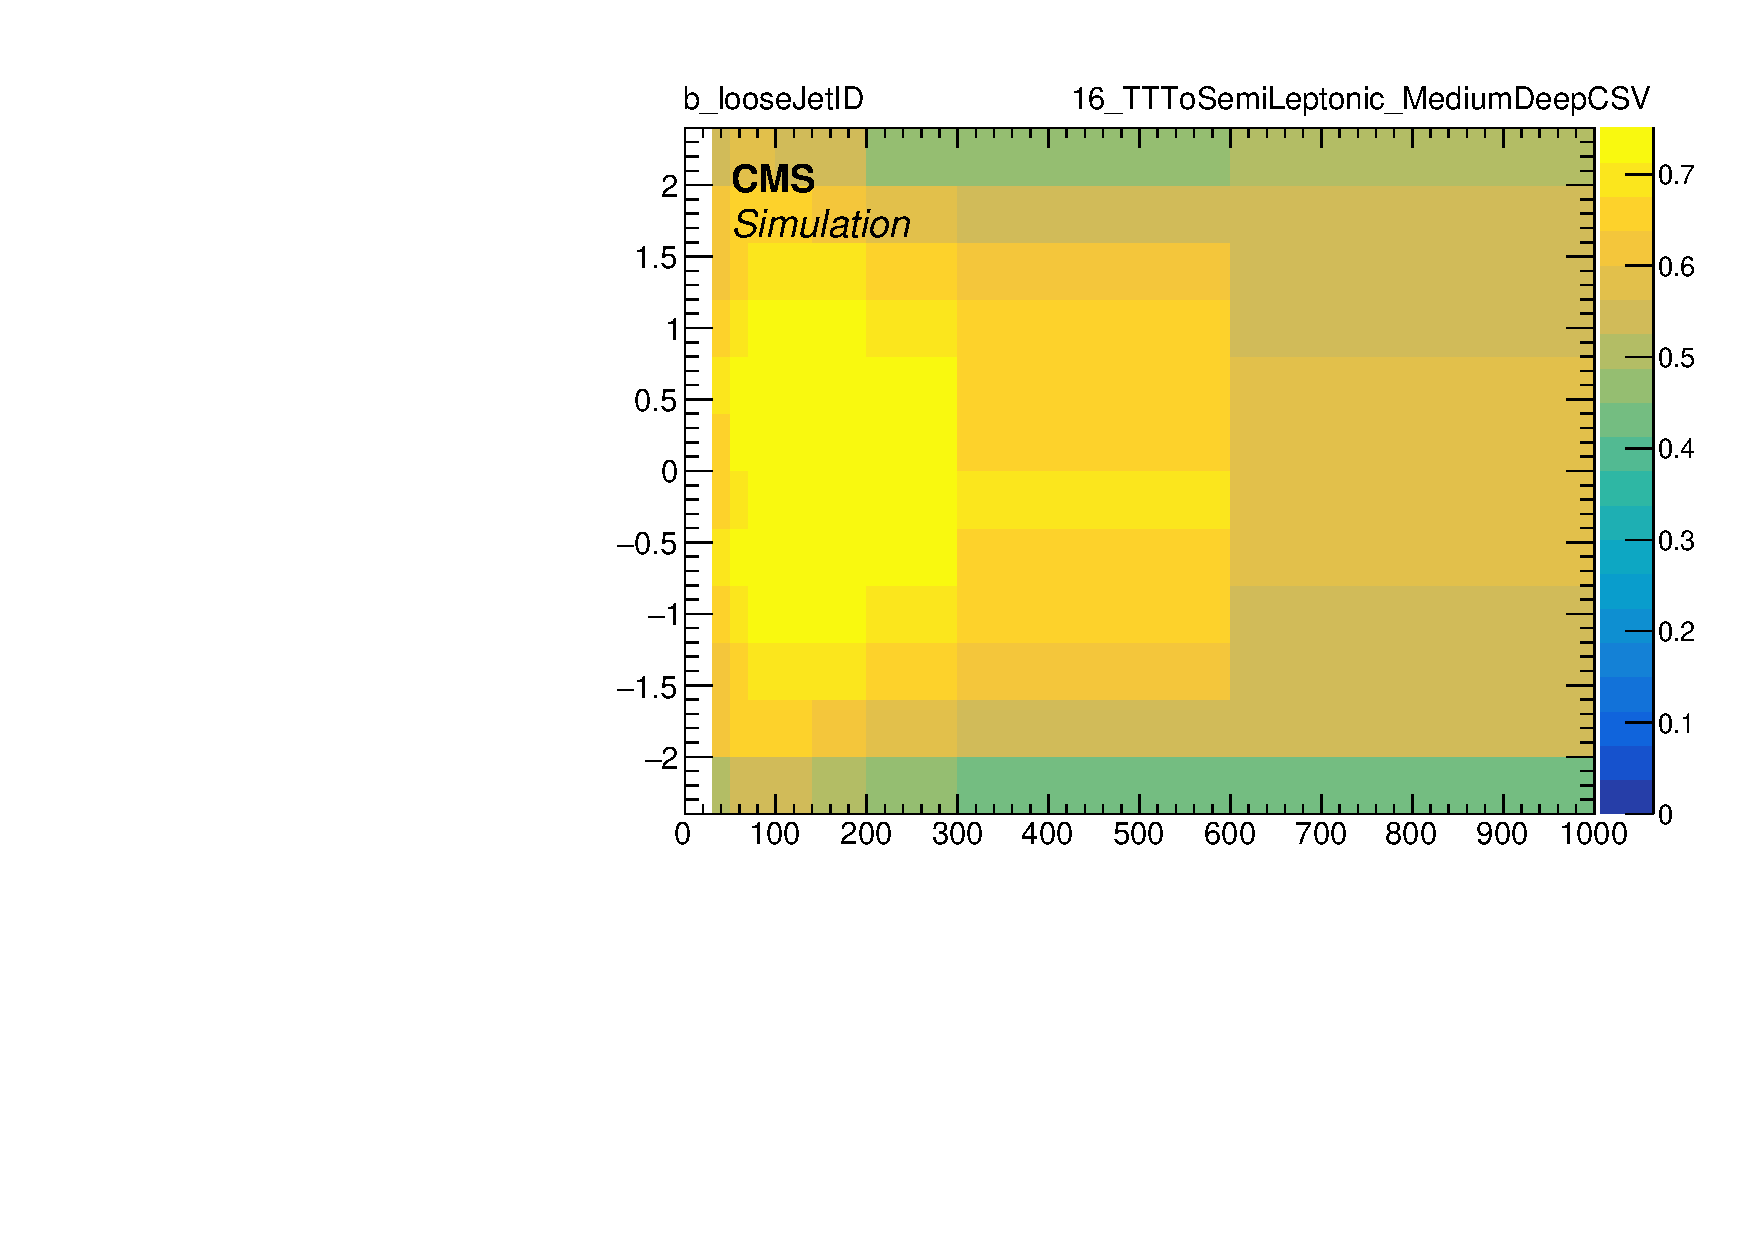
\includegraphics[width=0.4\textwidth]{figure/BtagEffPlot_16_TTToSemiLeptonic_eff2D_b_MediumDeepCSV.pdf}
    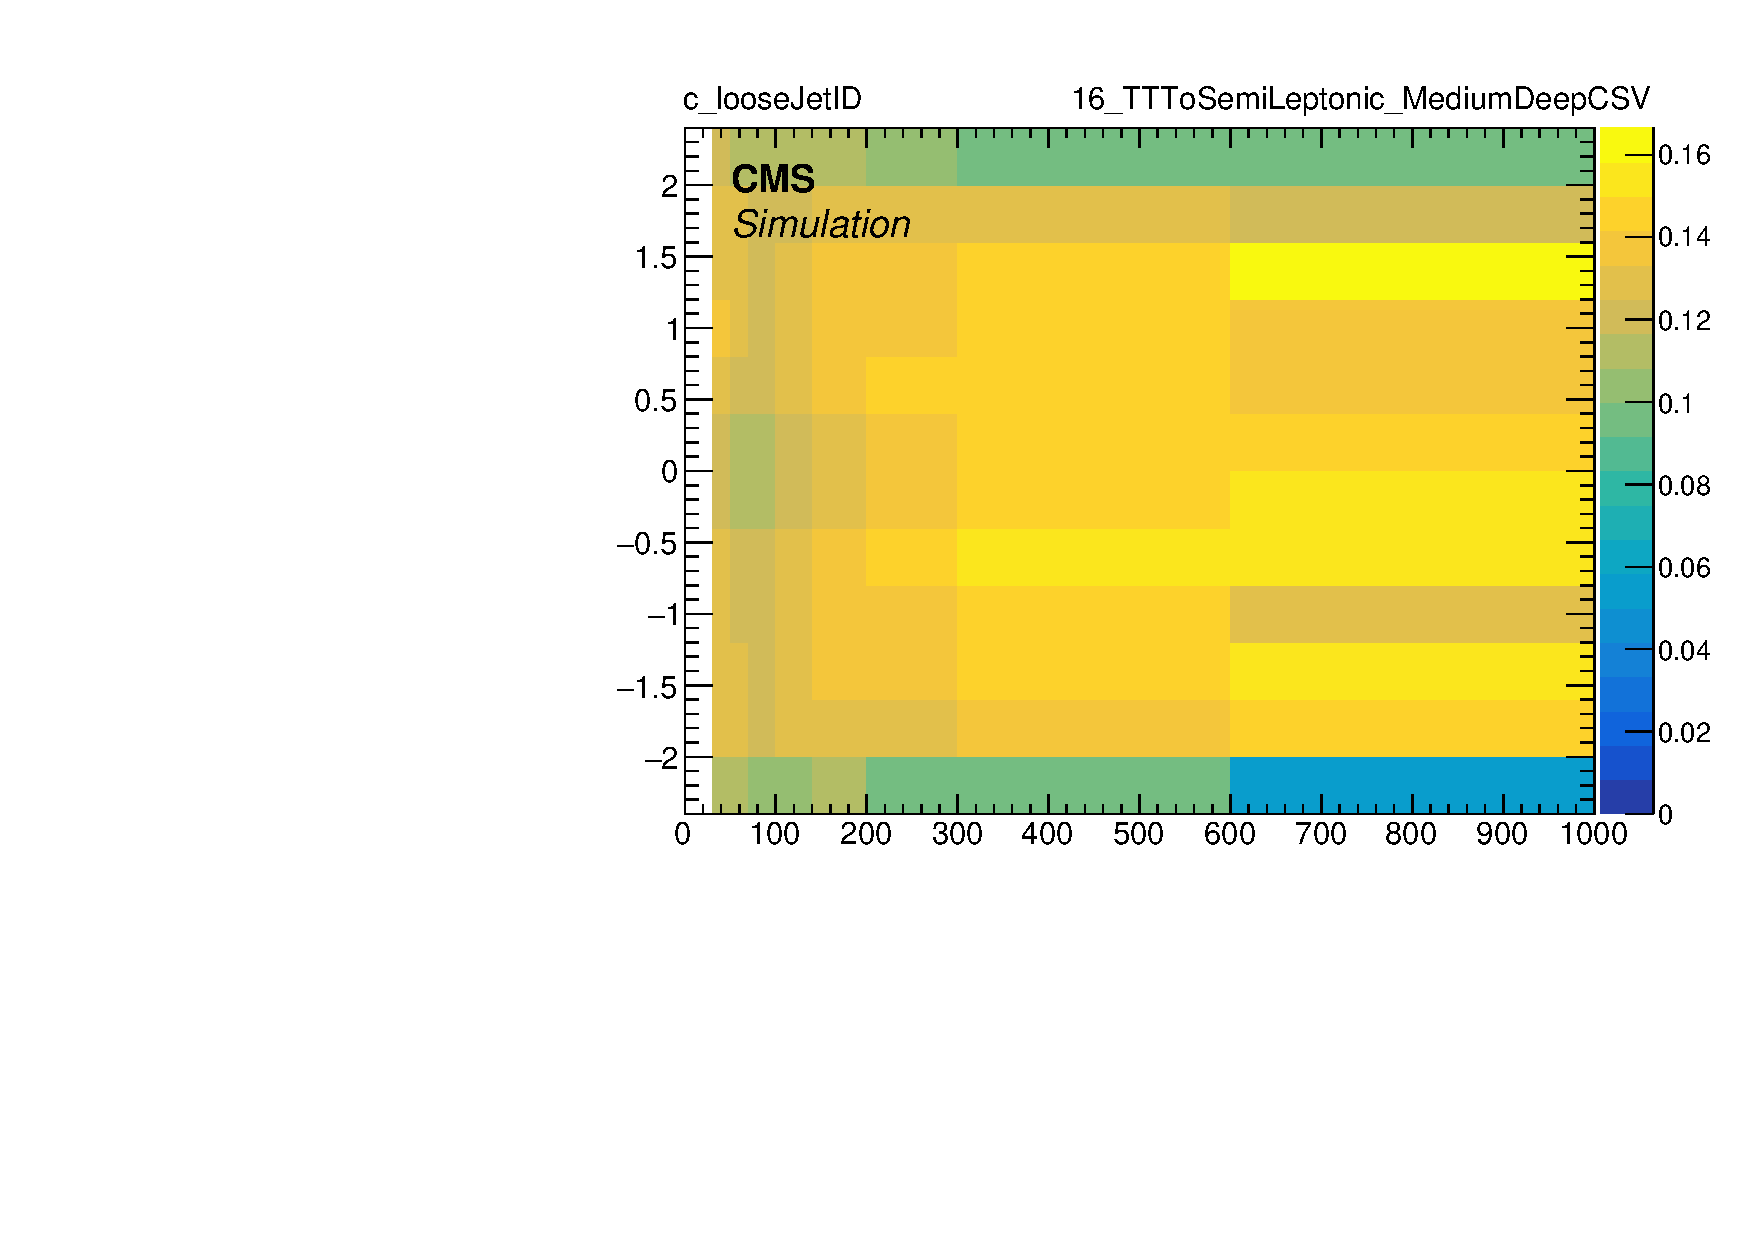
\includegraphics[width=0.4\textwidth]{figure/BtagEffPlot_16_TTToSemiLeptonic_eff2D_c_MediumDeepCSV.pdf}
    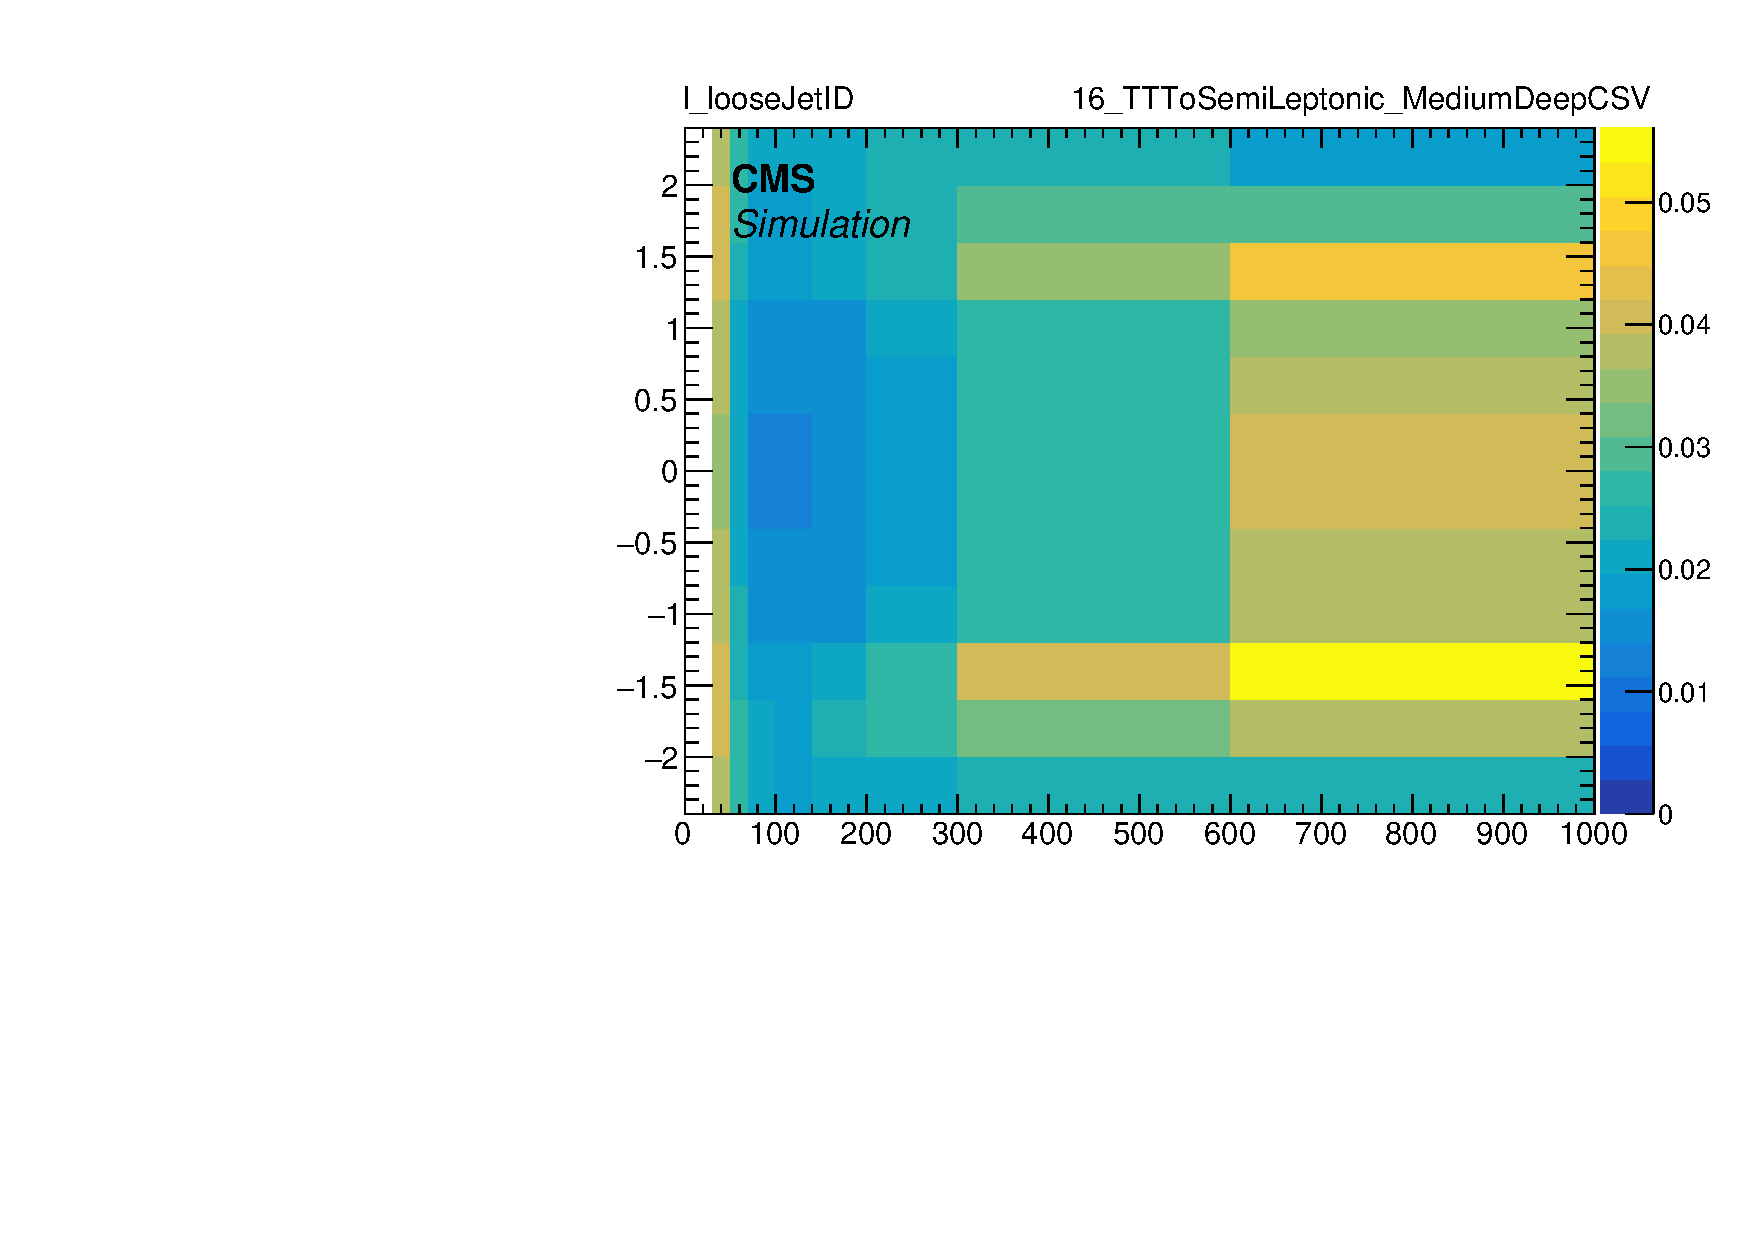
\includegraphics[width=0.4\textwidth]{figure/BtagEffPlot_16_TTToSemiLeptonic_eff2D_l_MediumDeepCSV.pdf}
    \caption[Display of \PQb tagging efficiency of 2016 \ttbar samples.]
    {
        Display of \PQb tagging efficiency of 2016 \ttbar samples for \PQb jet (left), \PQc jet (medium), and light jet (right) as functions of the jet \PT and jet $\eta$.
    }
    \label{fig:reco_beff16}
\end{figure}
\begin{figure}\centering
    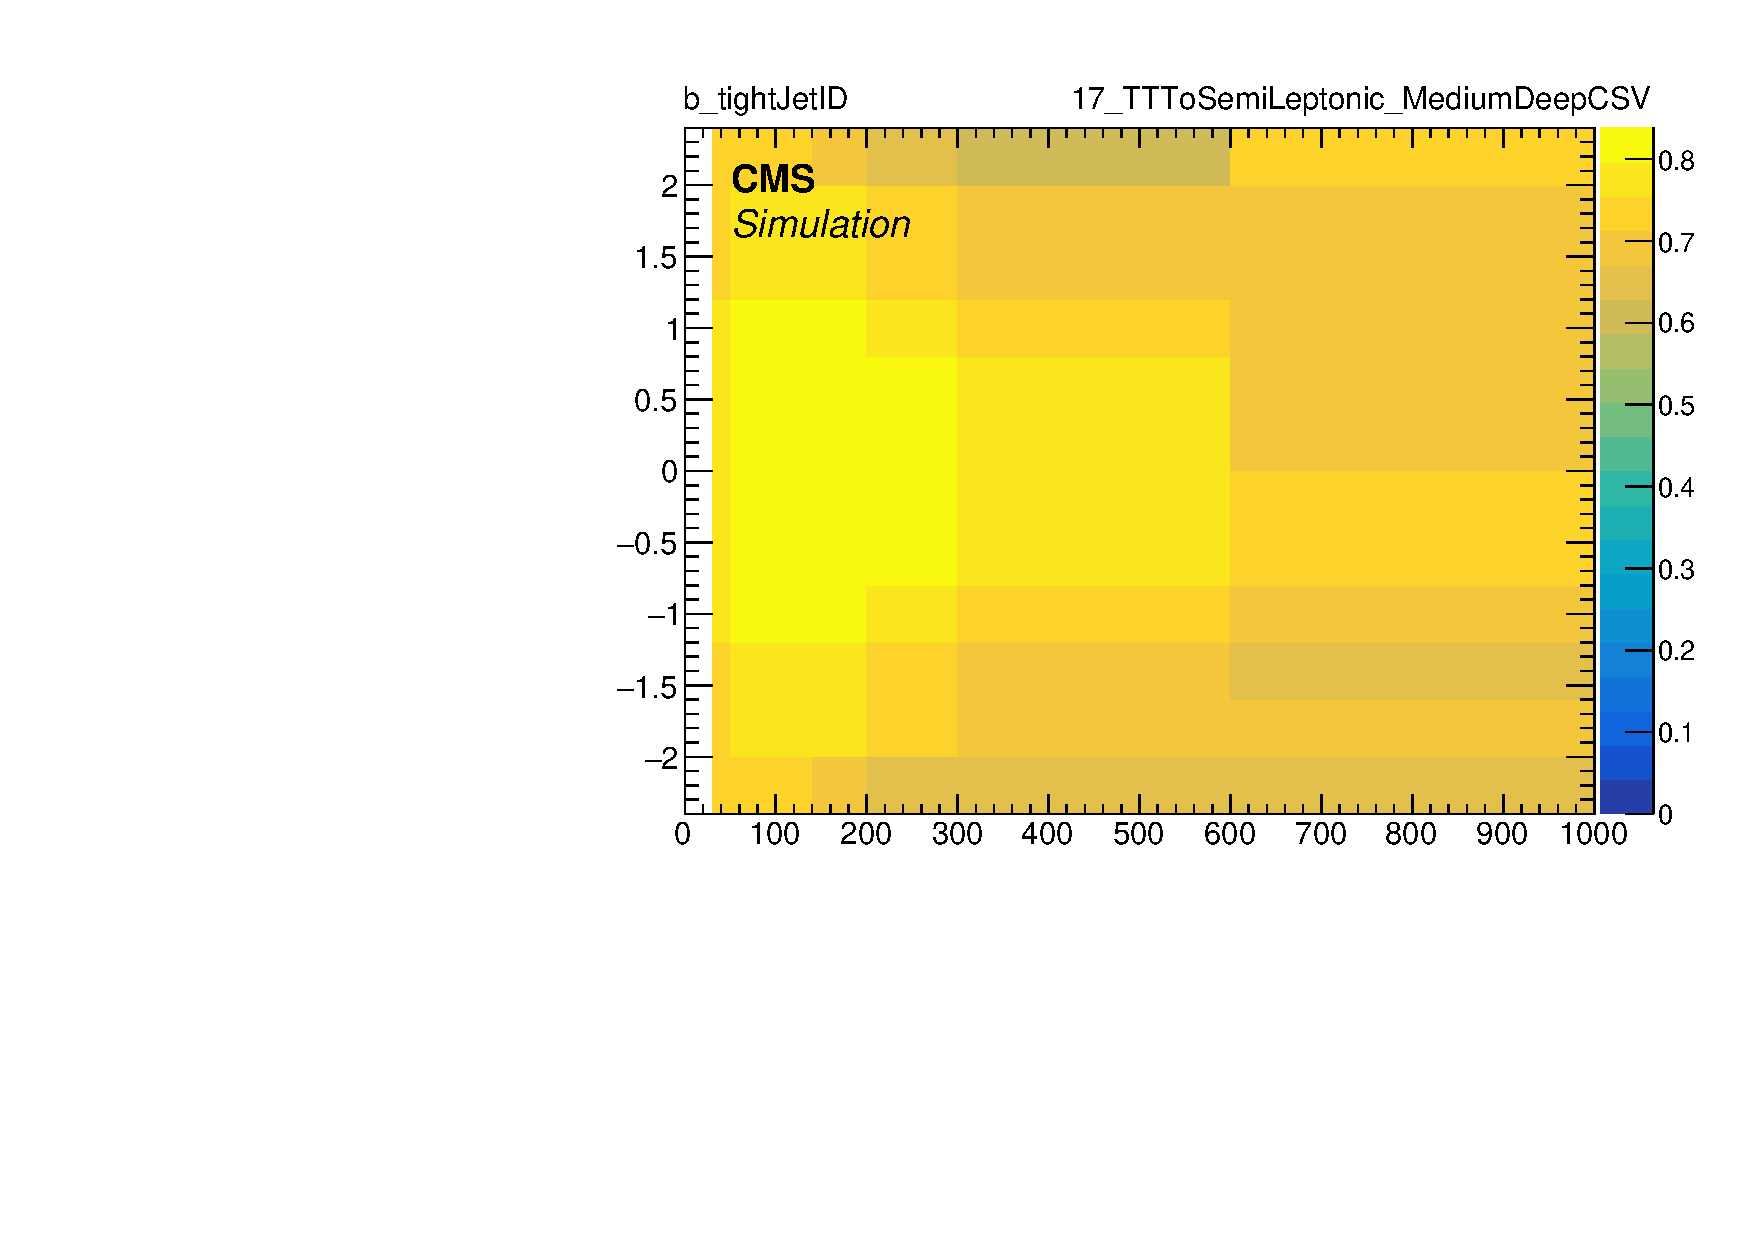
\includegraphics[width=0.4\textwidth]{figure/BtagEffPlot_17_TTToSemiLeptonic_eff2D_b_MediumDeepCSV.pdf}
    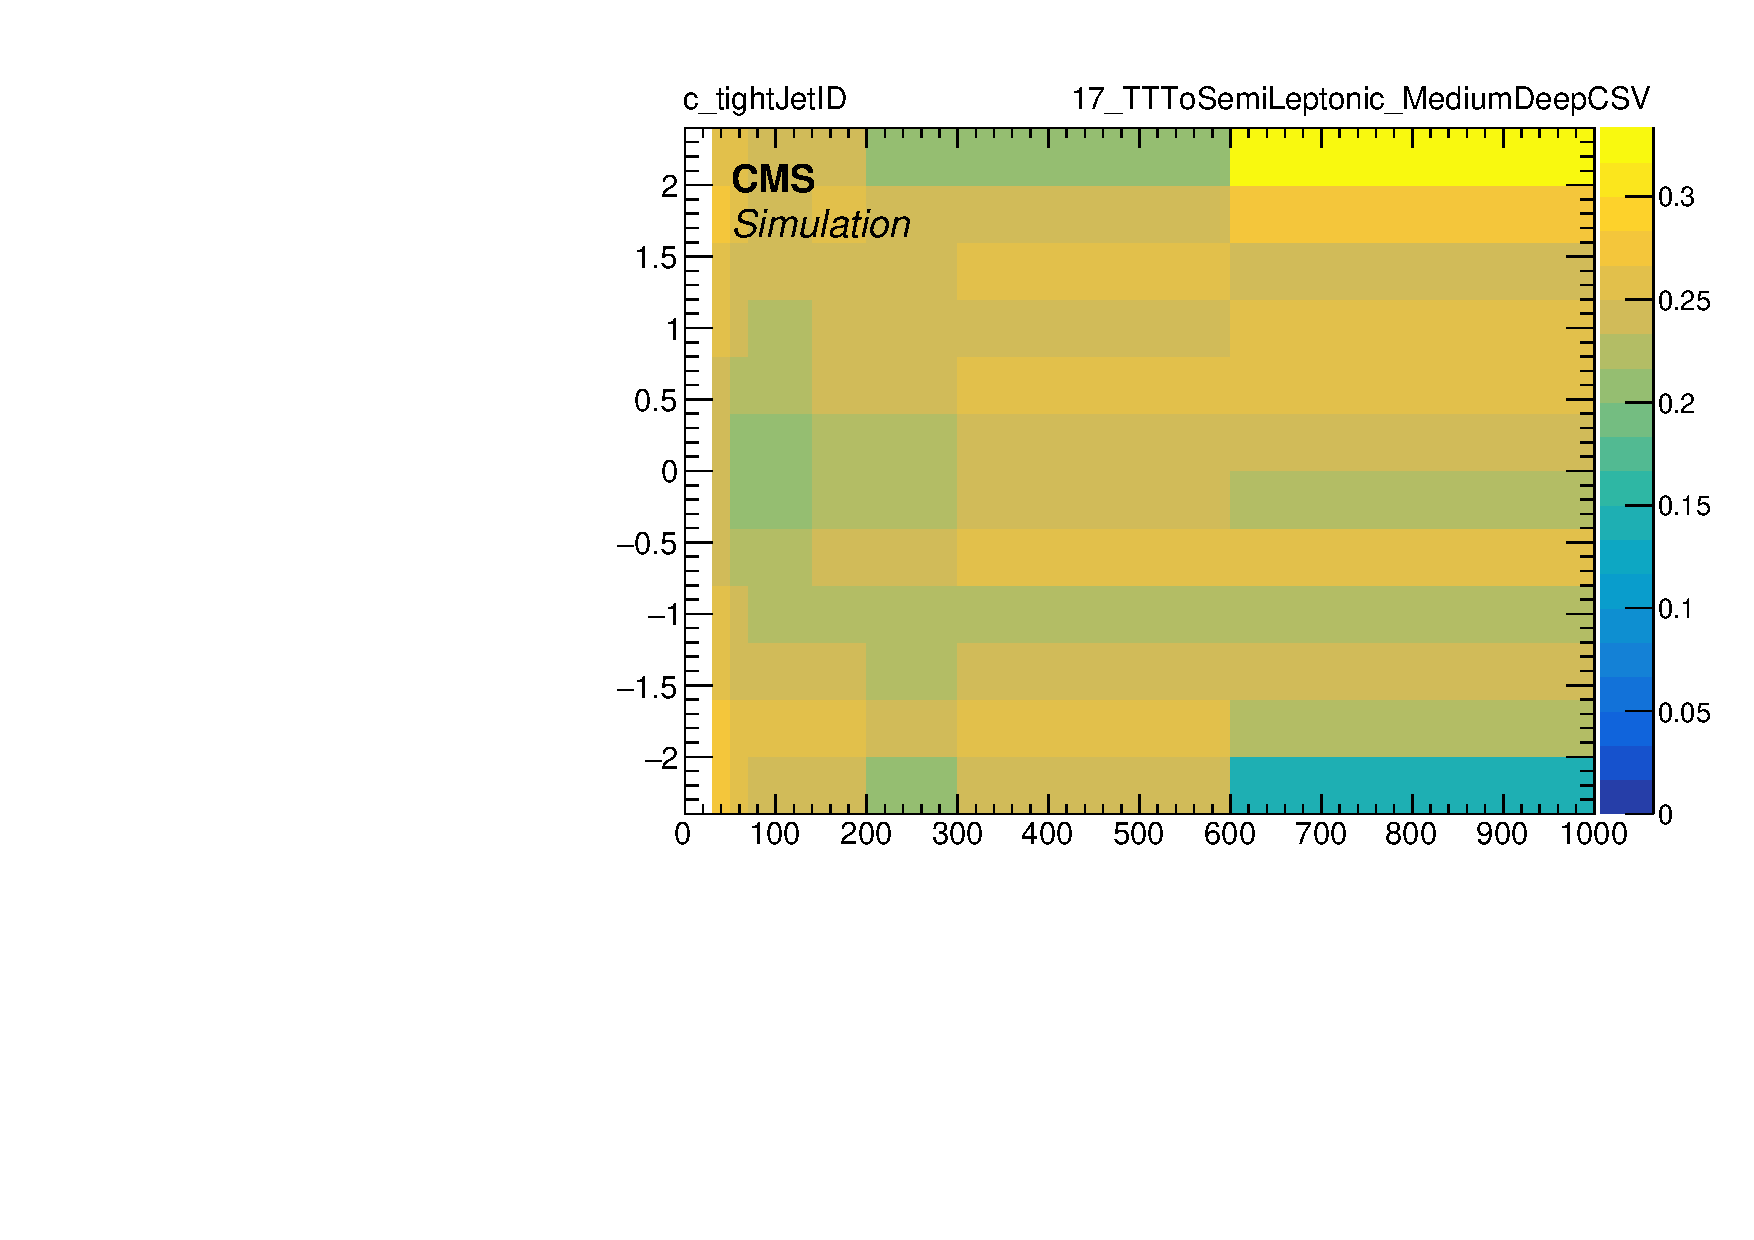
\includegraphics[width=0.4\textwidth]{figure/BtagEffPlot_17_TTToSemiLeptonic_eff2D_c_MediumDeepCSV.pdf}
    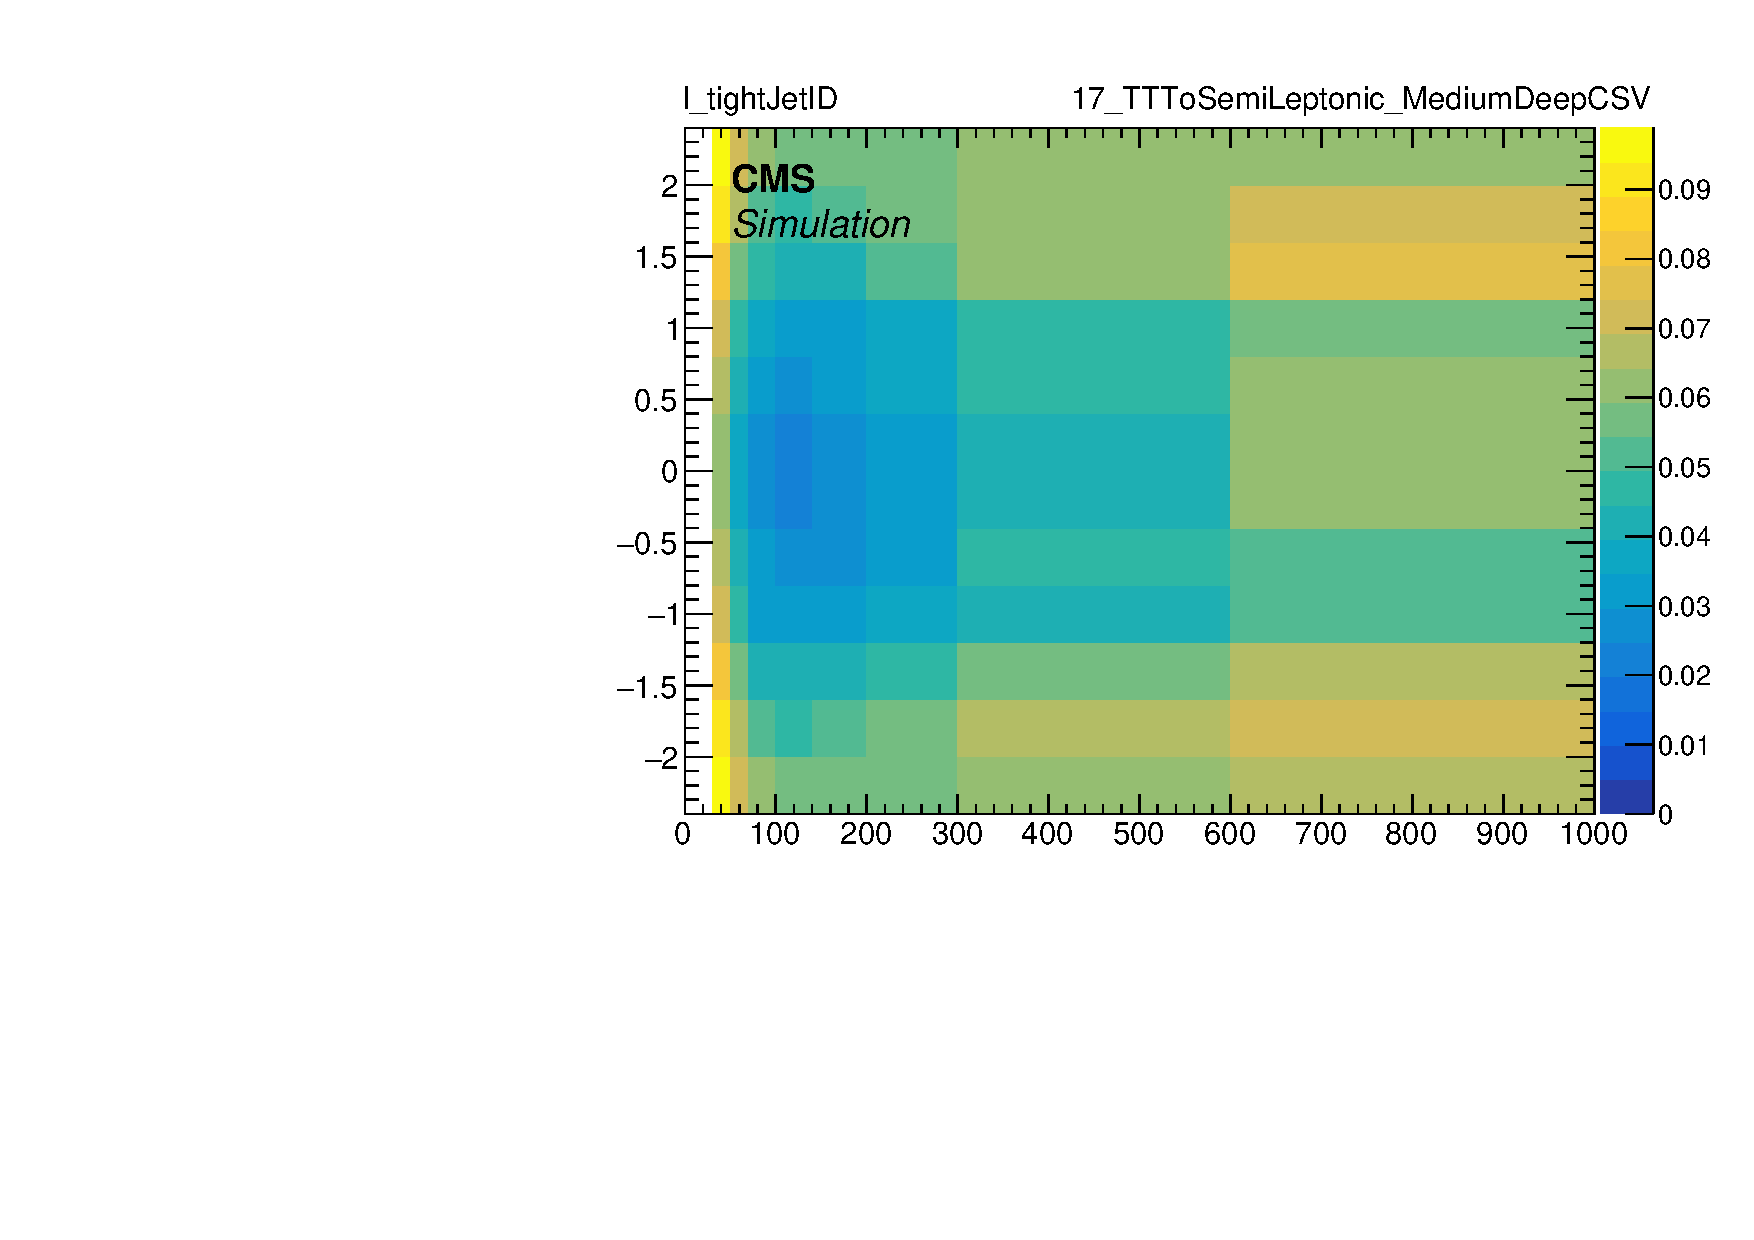
\includegraphics[width=0.4\textwidth]{figure/BtagEffPlot_17_TTToSemiLeptonic_eff2D_l_MediumDeepCSV.pdf}
    \caption[Display of \PQb tagging efficiency of 2017 \ttbar samples.]
    {
        Display of \PQb tagging efficiency of 2017 \ttbar samples for \PQb jet (left), \PQc jet (medium), and light jet (right) as functions of the jet \PT and jet $\eta$.
    }
    \label{fig:reco_beff17}
\end{figure}
\begin{figure}\centering
    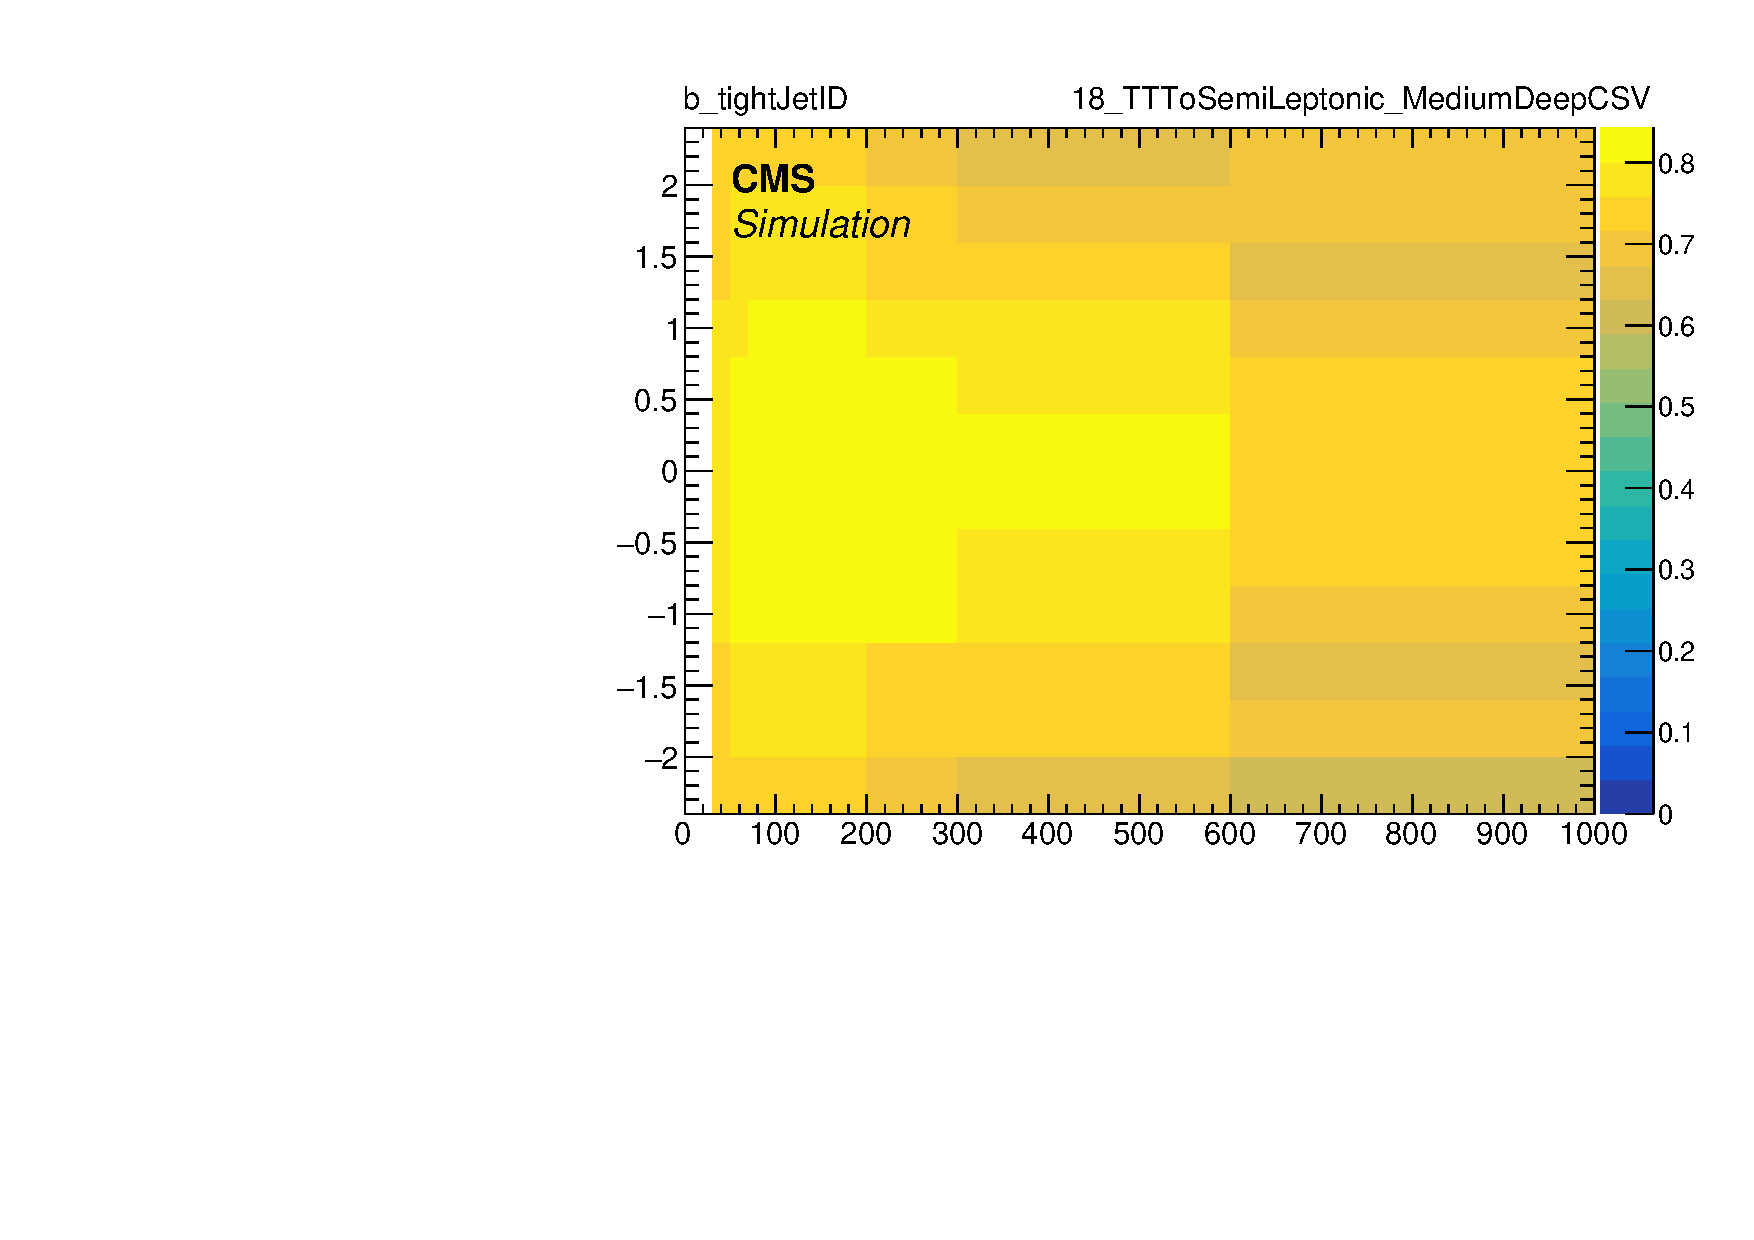
\includegraphics[width=0.4\textwidth]{figure/BtagEffPlot_18_TTToSemiLeptonic_eff2D_b_MediumDeepCSV.pdf}
    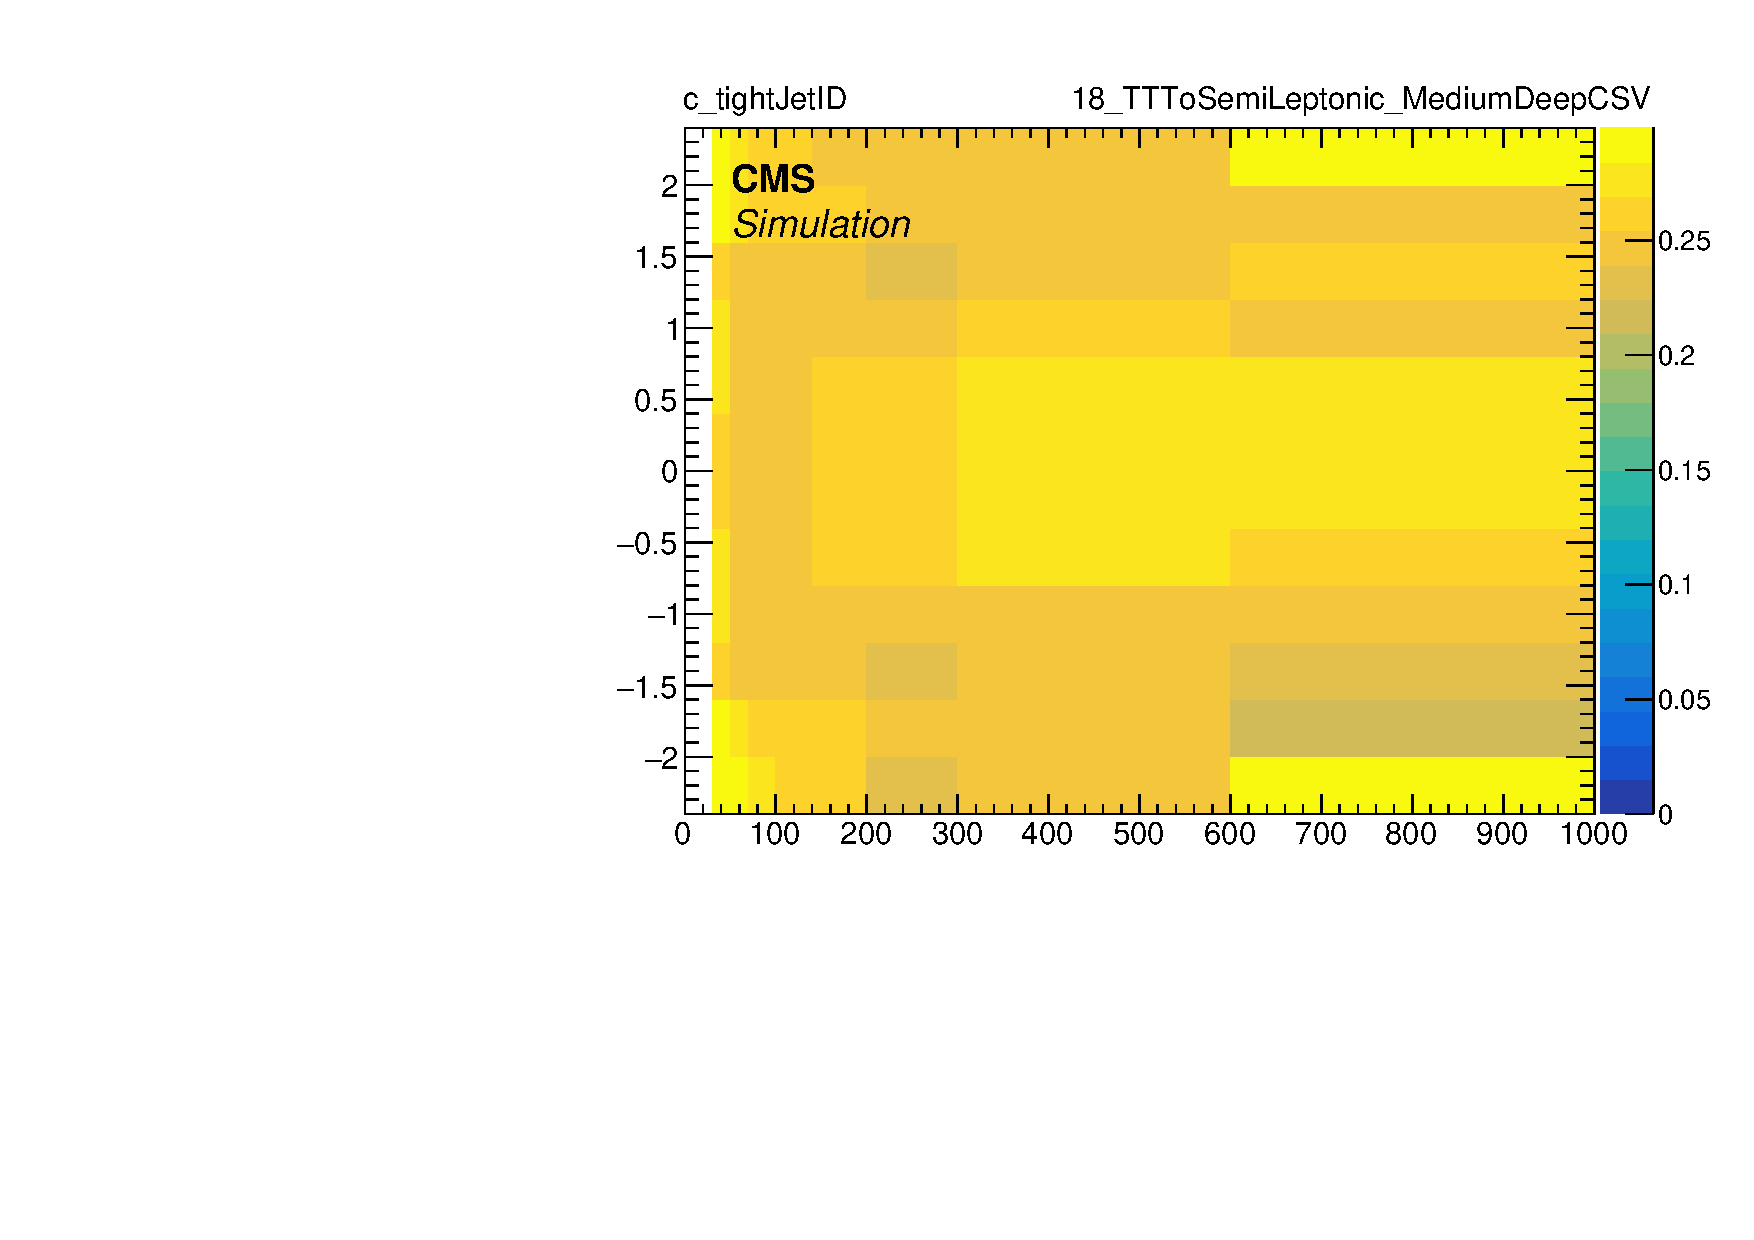
\includegraphics[width=0.4\textwidth]{figure/BtagEffPlot_18_TTToSemiLeptonic_eff2D_c_MediumDeepCSV.pdf}
    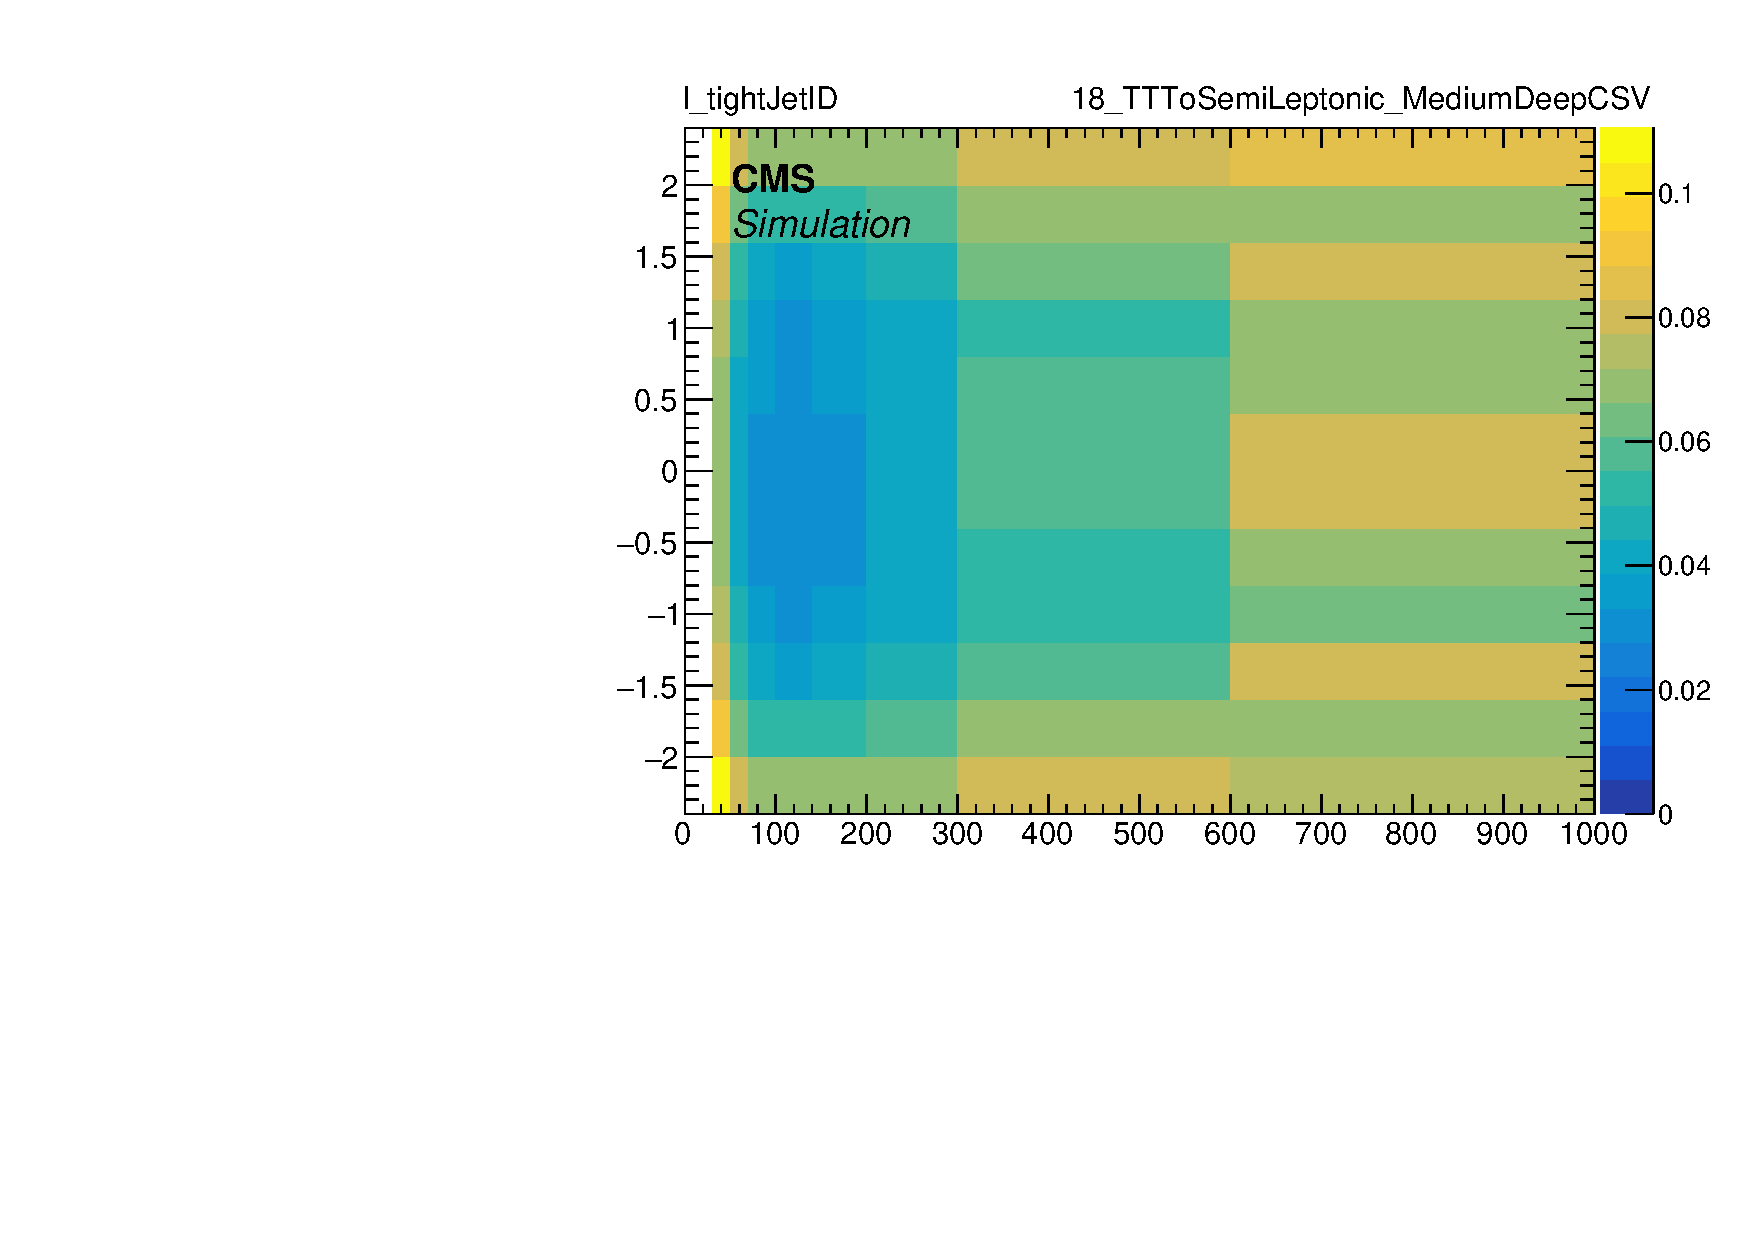
\includegraphics[width=0.4\textwidth]{figure/BtagEffPlot_18_TTToSemiLeptonic_eff2D_l_MediumDeepCSV.pdf}
    \caption[Display of \PQb tagging efficiency of 2018 \ttbar samples.]
    {
        Display of \PQb tagging efficiency of 2018 \ttbar samples for \PQb jet (left), \PQc jet (medium), and light jet (right) as functions of the jet \PT and jet $\eta$.
    }
    \label{fig:reco_beff18}
\end{figure}

\subsection{Pileup re-weighting}
Pileup in data is calculated by comparing the instantaneous luminosity of the proton beams with the total inelastic cross section of pp interaction.
On the other hand, the pileup in simulation is implemented by injecting additional soft interactions other than the main hard processes according to the expected pileup distribution.
However, the simulation typically starts before the actual data taking, and thus the expected pileup distribution might be different from the actual pileup distribution.
Such discrepancies are considered and corrected by re-weighting the simulated events to the actual pileup distribution.


\chapter{Event selection}
    \section{Trigger}
    The event selection criteria are based on the lepton+jets channel signature of the \ttbar process.
The signal events are required to contain one reconstructed lepton, and at least four reconstructed jets, including two \PQb-tagged jets (defined below) originating from \ttbar decays.
The events are further categorized into two channels based on the lepton flavor: either electron or muon.
Events are selected at the trigger level using single-lepton triggers, which require the presence of an isolated lepton above a \PT threshold in the range 24--35\GeV, depending on the year, and $\abseta < 2.4$.
The same trigger selection is applied to data and to the simulated samples.

    \section{Physical object selection}
    All physics objects are reconstructed offline using a particle-flow (PF) algorithm~\cite{CMS:particle_flow}.
The aim of the algorithm is to reconstruct all final-state particles (photons, charged and neutral hadrons, muons, and electrons) in the event, using combined information from the CMS detector.
The reconstructed vertex with the largest sum of object $\PT^2$ is taken to be the primary \pp interaction vertex.

Electron candidates are identified using the combination of the silicon tracker and the corresponding ECAL cluster information~\cite{CMS:el_PF}.
Electron energies are determined using the momenta derived from the electron track in the tracker system, the energy of the spatially compatible ECAL cluster, and the sum of all compatible bremsstrahlung photon energies.
In order to reject events with misidentified electron candidates and candidates originating from photon conversions, additional electron identification requirements are applied.
A PF-based combined relative isolation, \Irel, is defined as the \PT sum of all neutral hadron, charged hadron, and photon candidates within a cone of size $\DR = \sqrt{\smash[b]{(\Delta\eta)^2+(\Delta\phi)^2}} < 0.4$ (where $\phi$ is the azimuthal angle in radians) around the lepton direction, divided by the lepton \PT, with a correction to suppress the residual effect of pileup~\cite{CMS:el_reliso}.
The isolated electron candidate is required to have $\PT>38\GeV$, $\abseta < 2.4$, and $\Irel < 0.0287+0.506/\PT$ ($0.0445+0.963/\PT$) in the barrel (endcaps), with \PT in \GeV.
Due to reduced reconstruction efficiency, the gap ($1.44 < \abseta < 1.57$) between the barrel and endcap parts of the ECAL is excluded.
Events with additional electrons satisfying a looser set of selection criteria with a lower-\PT threshold and a looser isolation requirement are rejected to reduce the background contribution (\eg, from DY production).

Muon candidates are reconstructed using information obtained in the tracker, combined with the muon system~\cite{CMS:mu_PF}.
Identification methods are applied to reject muon candidates that are misidentified or muons that originated from decay-in-flight.
The isolated muon candidate is required to have $\PT > 30\GeV$, $\abseta < 2.4$, and $\Irel < 0.15$.
Events with additional muons satisfying a looser set of selection criteria are rejected as well.

Jets are clustered using the anti-\kt algorithm with a distance parameter of 0.4~\cite{CMS:fastjet, CMS:antikt}.
The jet \ptvec is defined as the vectorial sum of the momenta of all PF candidates in the jet anti-\kt clustering.
Pileup can contribute additional tracks and calorimetric energy depositions to the jet momentum.
To mitigate this effect, tracks identified as originating from pileup vertices are discarded, and an offset correction is applied to correct for remaining contributions from neutral particles from pileup~\cite{CMS:particle_flow}.
Corrections to the jet energy are applied as a function of jet \PT and $\eta$ by studying discrepancies between simulation and data.
At least four jets are required with $\PT > 30\GeV$, $\abseta < 2.4$, and angular separation relative to the selected lepton of $\DR > 0.4$.
Jets are identified as arising from the hadronization of \PQb quarks, denoted as either \PQb-tagged jets or \PQb jets, using the deep-learned combined secondary-vertex algorithm (\DeepCSV).
This combines the information for a given jet from track impact parameters and secondary vertices into a model optimized through a deep neural network.
The selected working point has a signal identification efficiency of 68\%, with a probability to misidentify \PQc quark, and light-flavor quark and gluon jets as \PQb jets of approximately 12 and 1.1\% in \ttbar events, respectively~\cite{CMS:bjet_eff}.

The top quark and antiquark candidates associated with \PW bosons decaying to \qqbar are reconstructed using one of the \PQb-tagged jets and two non-\PQb-tagged jets in the event through a \chisq algorithm that uses the top quark and \PW boson masses as constraints~\cite{CMS:sorting_algo}.
Those candidates are chosen from the combination having the lowest \chisq value, with the \chisq defined as
\begin{linenomath}\begin{equation}
    \chisq = \left(\frac{\mjjb-\Mt}{\sigt}\right)^2 + \left(\frac{\mjj-\MW}{\sigW}\right)^2,
\end{equation}\end{linenomath}
where \mjjb is the invariant mass of the two non-\PQb-tagged jets and the associated \PQb-tagged jet; \Mt and \sigt are the default top quark mass and average top quark invariant mass resolution of 172.5 and 16.3\GeV, respectively; \mjj is the invariant mass of the two non-\PQb-tagged jets; and \MW and \sigW are the default \PW boson mass and average \PW boson invariant mass resolution of 82.9 and 9.5\GeV, respectively~\cite{CPVtop:chi2value}.
The other \PQb-tagged jet associated with the leptonically decaying \PW boson candidate is assigned as being from the hadronization of a bottom quark or antiquark based on the charge sign of the lepton.
The events can be further categorized into three different types: the correct type represents the events with \PQb jets correctly assigned, the misidentified type stands for the events with \PQb jets are swapped, and the mistag type represents the events with one or all of the selected \PQb jets matched to the wrong objects.
Juding from Fig.~\ref{fig:bbsep_rate}, events with higher minimum \chisq are mainly composed of misidentified and mistag types.
The event purity of the correctly assigned \PQb jets can be raised after imposing an upper bound on the minimum \chisq.
An upper bound of 20 on minimum \chisq achieves around $70\%$ event efficiency with $60\%$ correctly assigned \PQb jets as indicated in Fig.~\ref{fig:bbsep_uppercut}.

However, from simulation it is found that when the invariant mass of the combined isolated lepton and associated \PQb-tagged jet (\Mlb) is greater than 150\GeV, the events have a large fraction of incorrect \PQb jet assignments as shown in Fig.~\ref{fig:opt_lept}.
Therefore, from studies of the simulated \ttbar sample, further requirements of $\chisq < 20$ and $\Mlb < 150\GeV$ are imposed.
This improves the fraction of correctly assigned \PQb jets to $\approx$74\%, while keeping $\approx$65\% of the \ttbar events as shown in Figs~\ref{fig:opt_cut}.

After these selection criteria, the purity of the \ttbar events is 95\%, with single top quark production contributing a background of 3\%.
The upper panels in Figs.~\ref{fig:el_obs_dist} and~\ref{fig:mu_obs_dist} show the distributions of the CP observables for the electron and muon channels, respectively.
The middle panels display the ratio of the data to the simulated distributions, which show reasonable agreement within the one-standard-deviation band.
The bottom panels present the ratio of the CEDM to the SM predictions for $\dtG = \pm 3$.
In these figures, the values of the CP observables are divided by \Mtcub to convert the units to \GeVns.
The systematic uncertainties shown in Figs.~\ref{fig:el_obs_dist} and~\ref{fig:mu_obs_dist}, as well as in later figures and tables, include all systematic uncertainties, except for those due to backgrounds.
The latter uncertainty contributes only to the final \Acp measurements instead of the number of signal events and will be discussed in detail in Section~\ref{sec:uncertainty}.
Table~\ref{tab:signal_region_expected_percentage} shows the predicted signal and background contributions to the signal events from simulation for the electron and muon channels.
The fraction of leptonic tau decays in the SM simulated \ttbar samples is about 0.3\% and the contribution is negligible in the final results.
The QCD and \ttbar multijet events are highly suppressed by the selection requirements and provide negligible contributions of around 0.2 and 0.05\%, respectively, to the signal events.
The estimation of the number of misidentified signal events coming from \ttbar decays to dilepton+jets is discussed in Section~\ref{sec:fitresult}.
\begin{figure}[p]
    \centering
    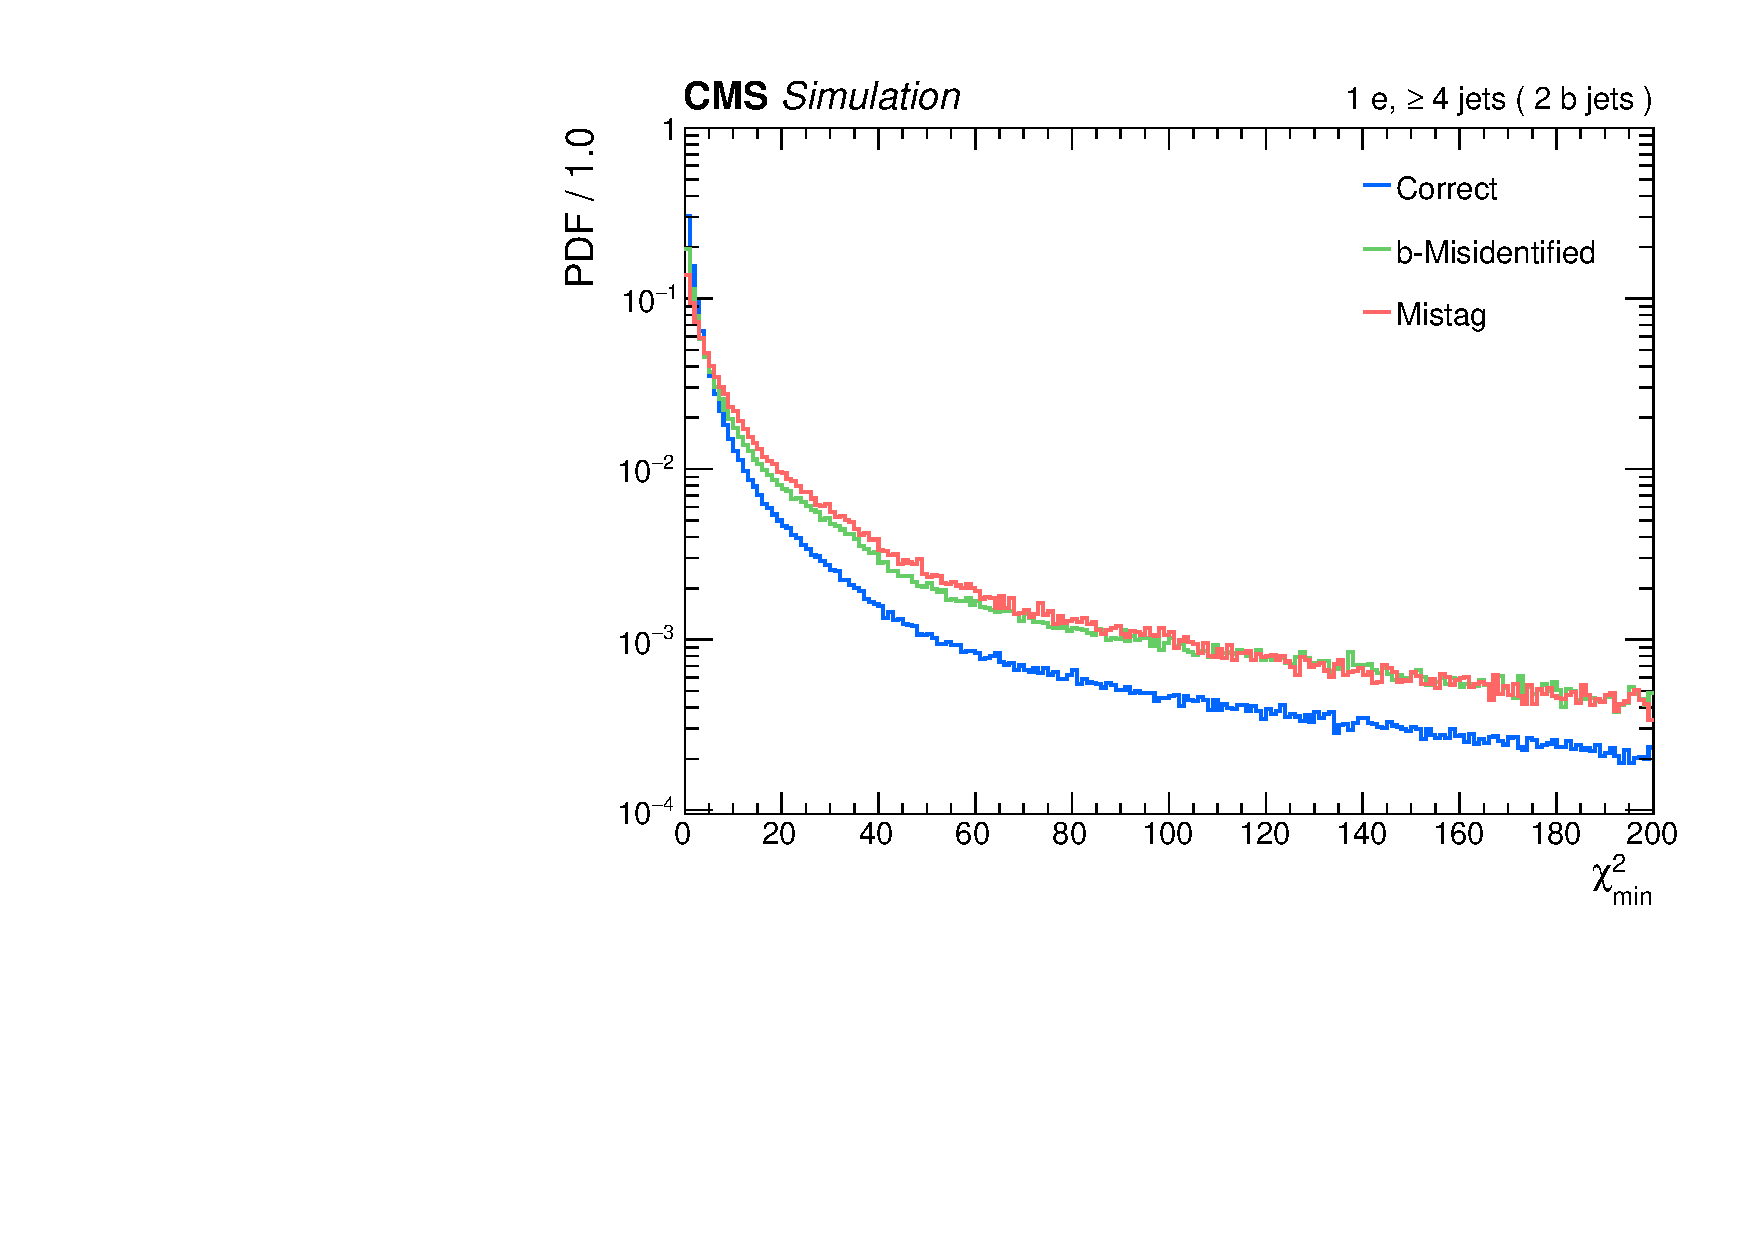
\includegraphics[width=0.45\textwidth]{figure/bbSep_16_el_Rate_PDF_bbSep.pdf}
    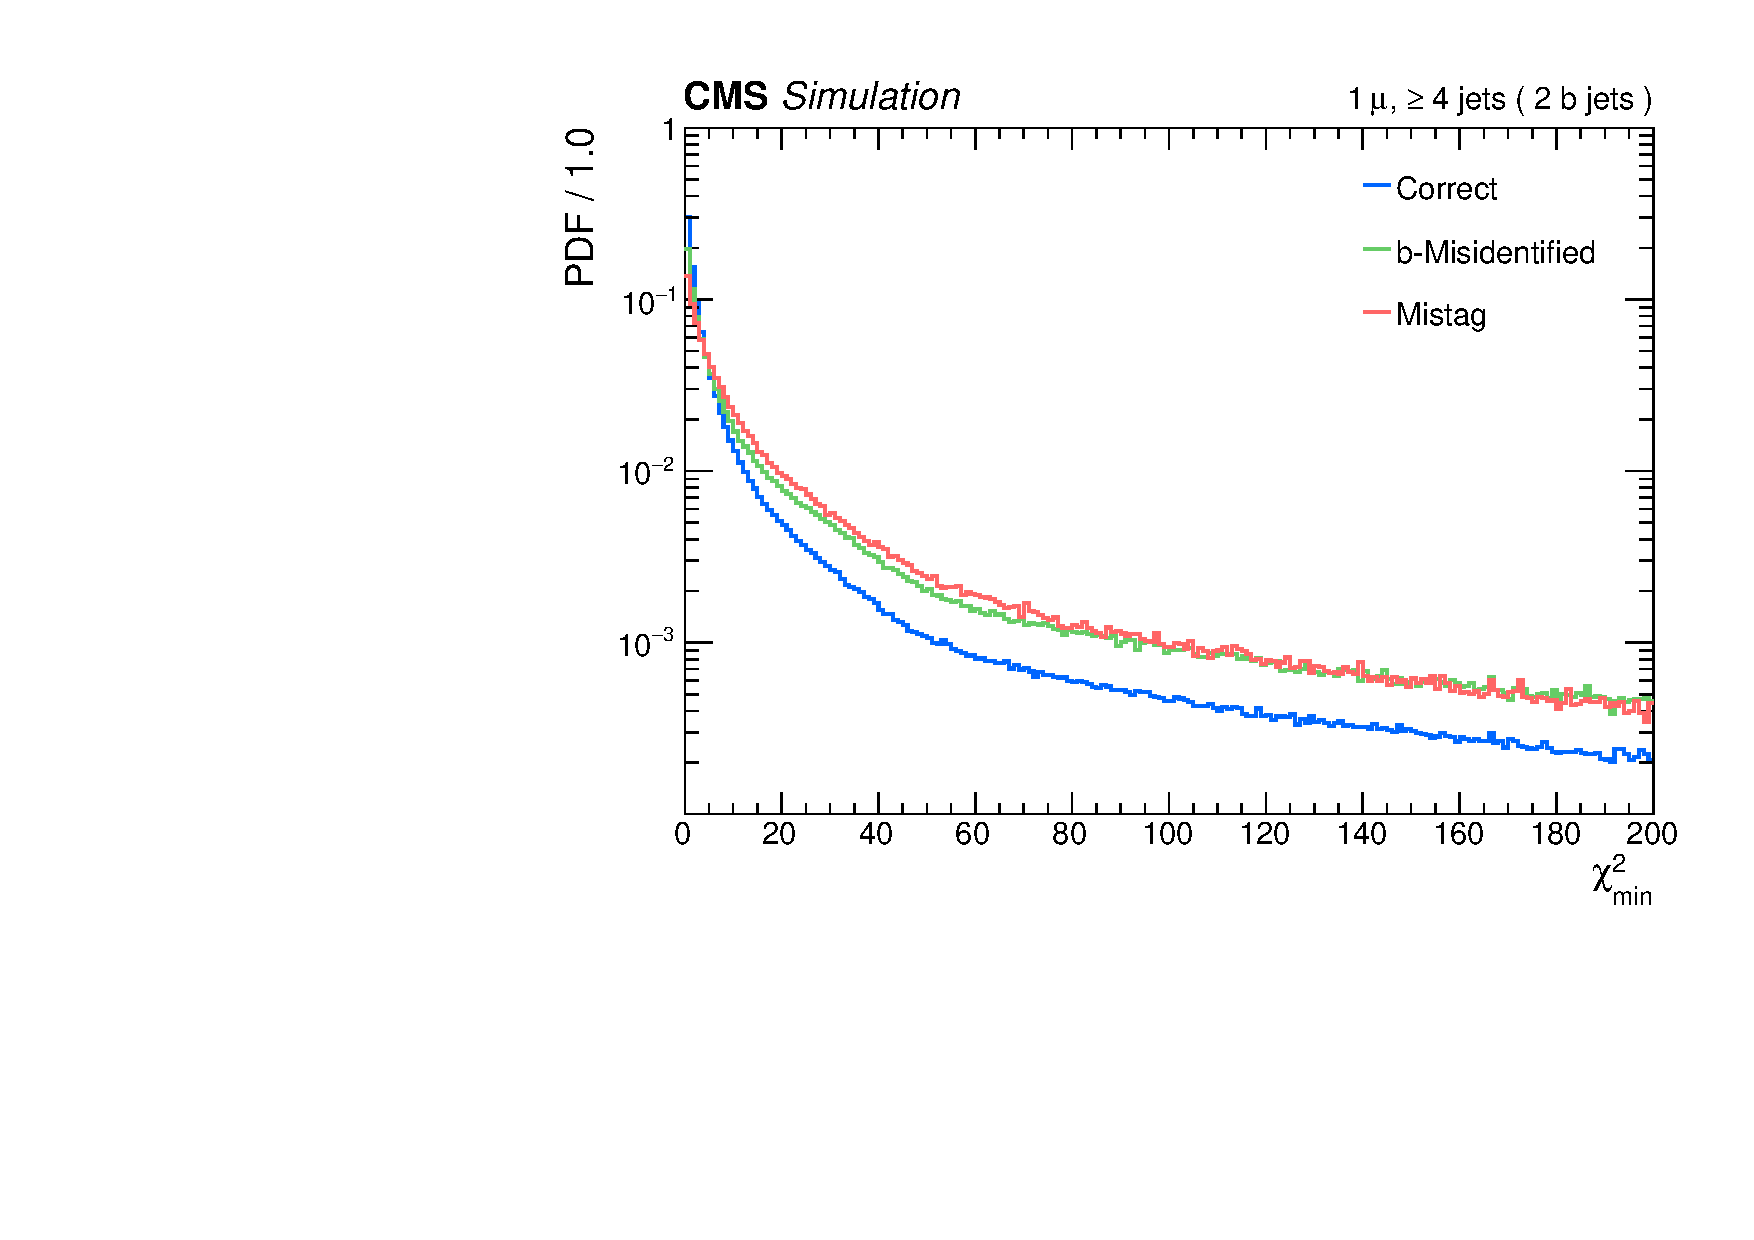
\includegraphics[width=0.45\textwidth]{figure/bbSep_16_mu_Rate_PDF_bbSep.pdf}
    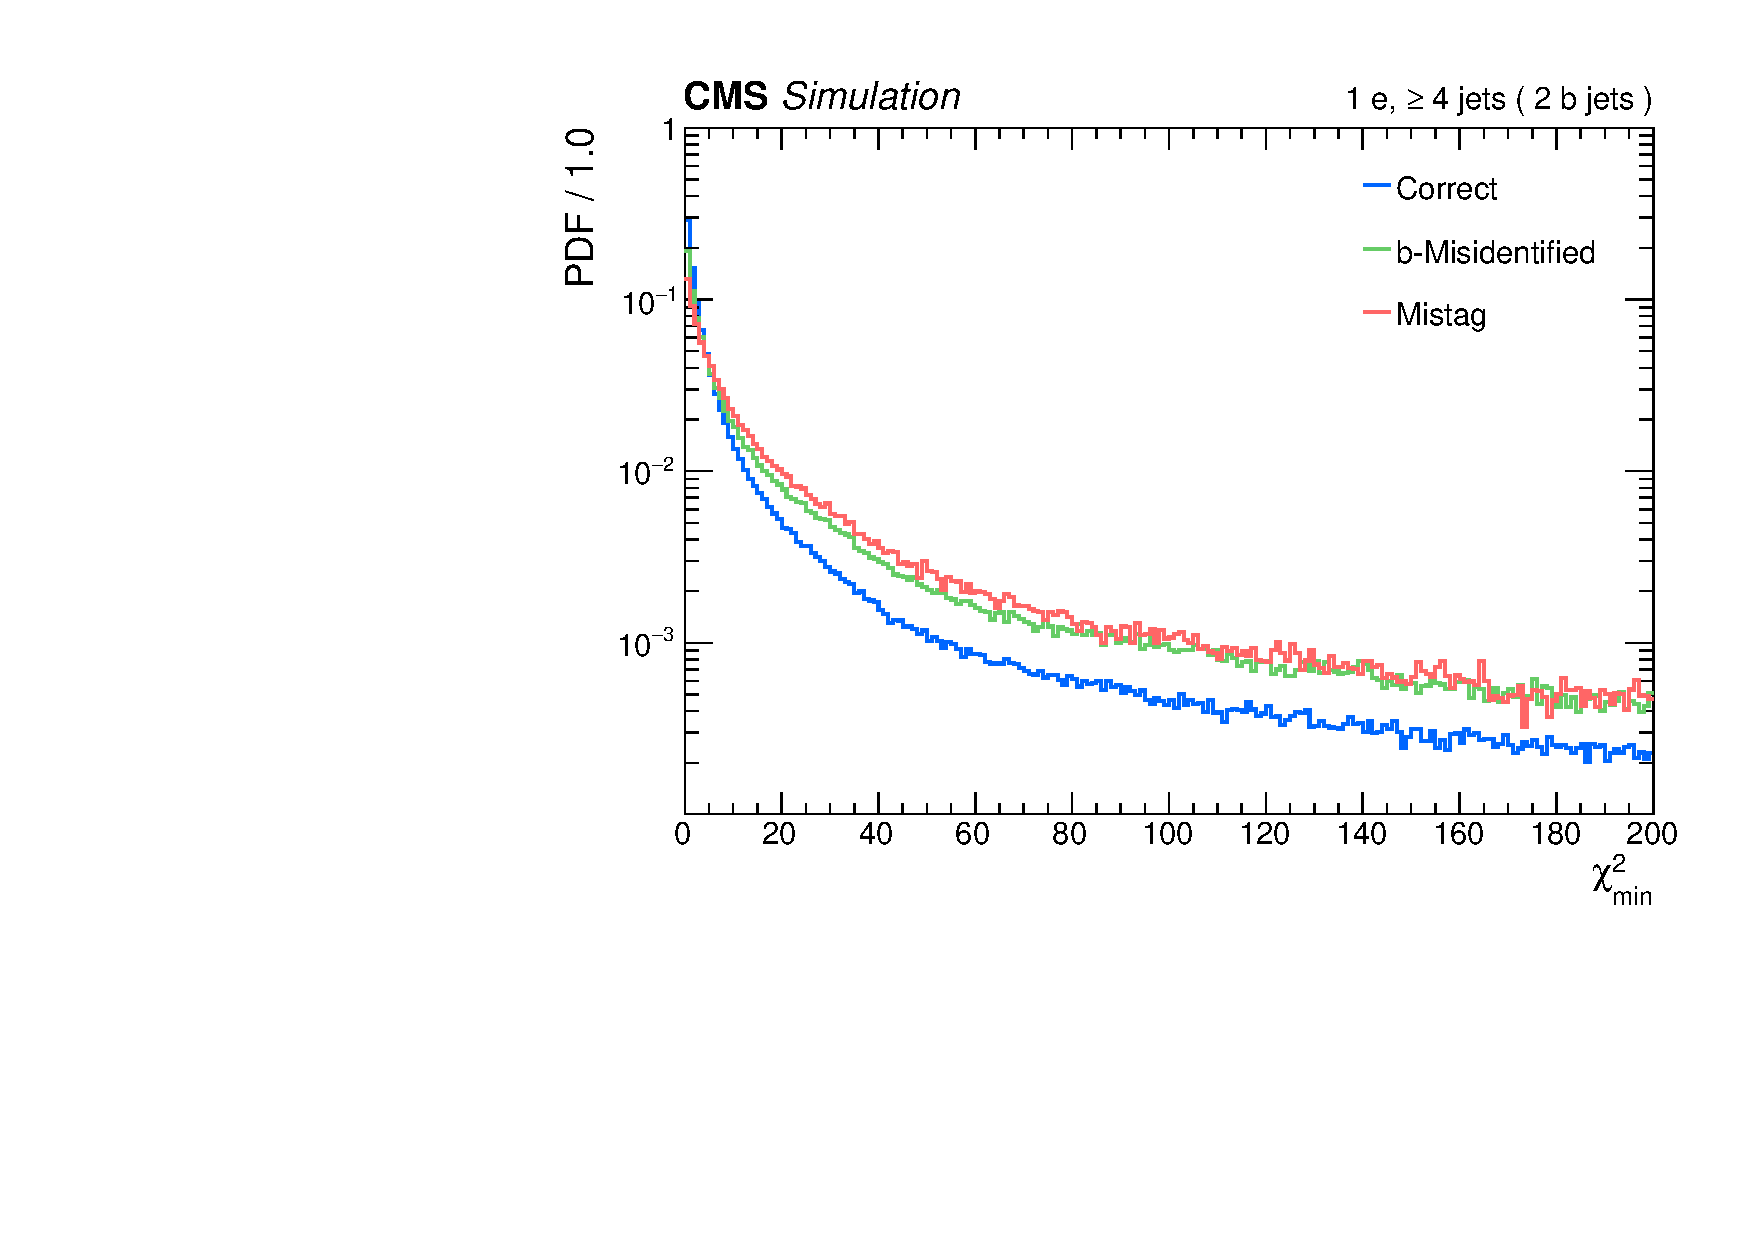
\includegraphics[width=0.45\textwidth]{figure/bbSep_17_el_Rate_PDF_bbSep.pdf}
    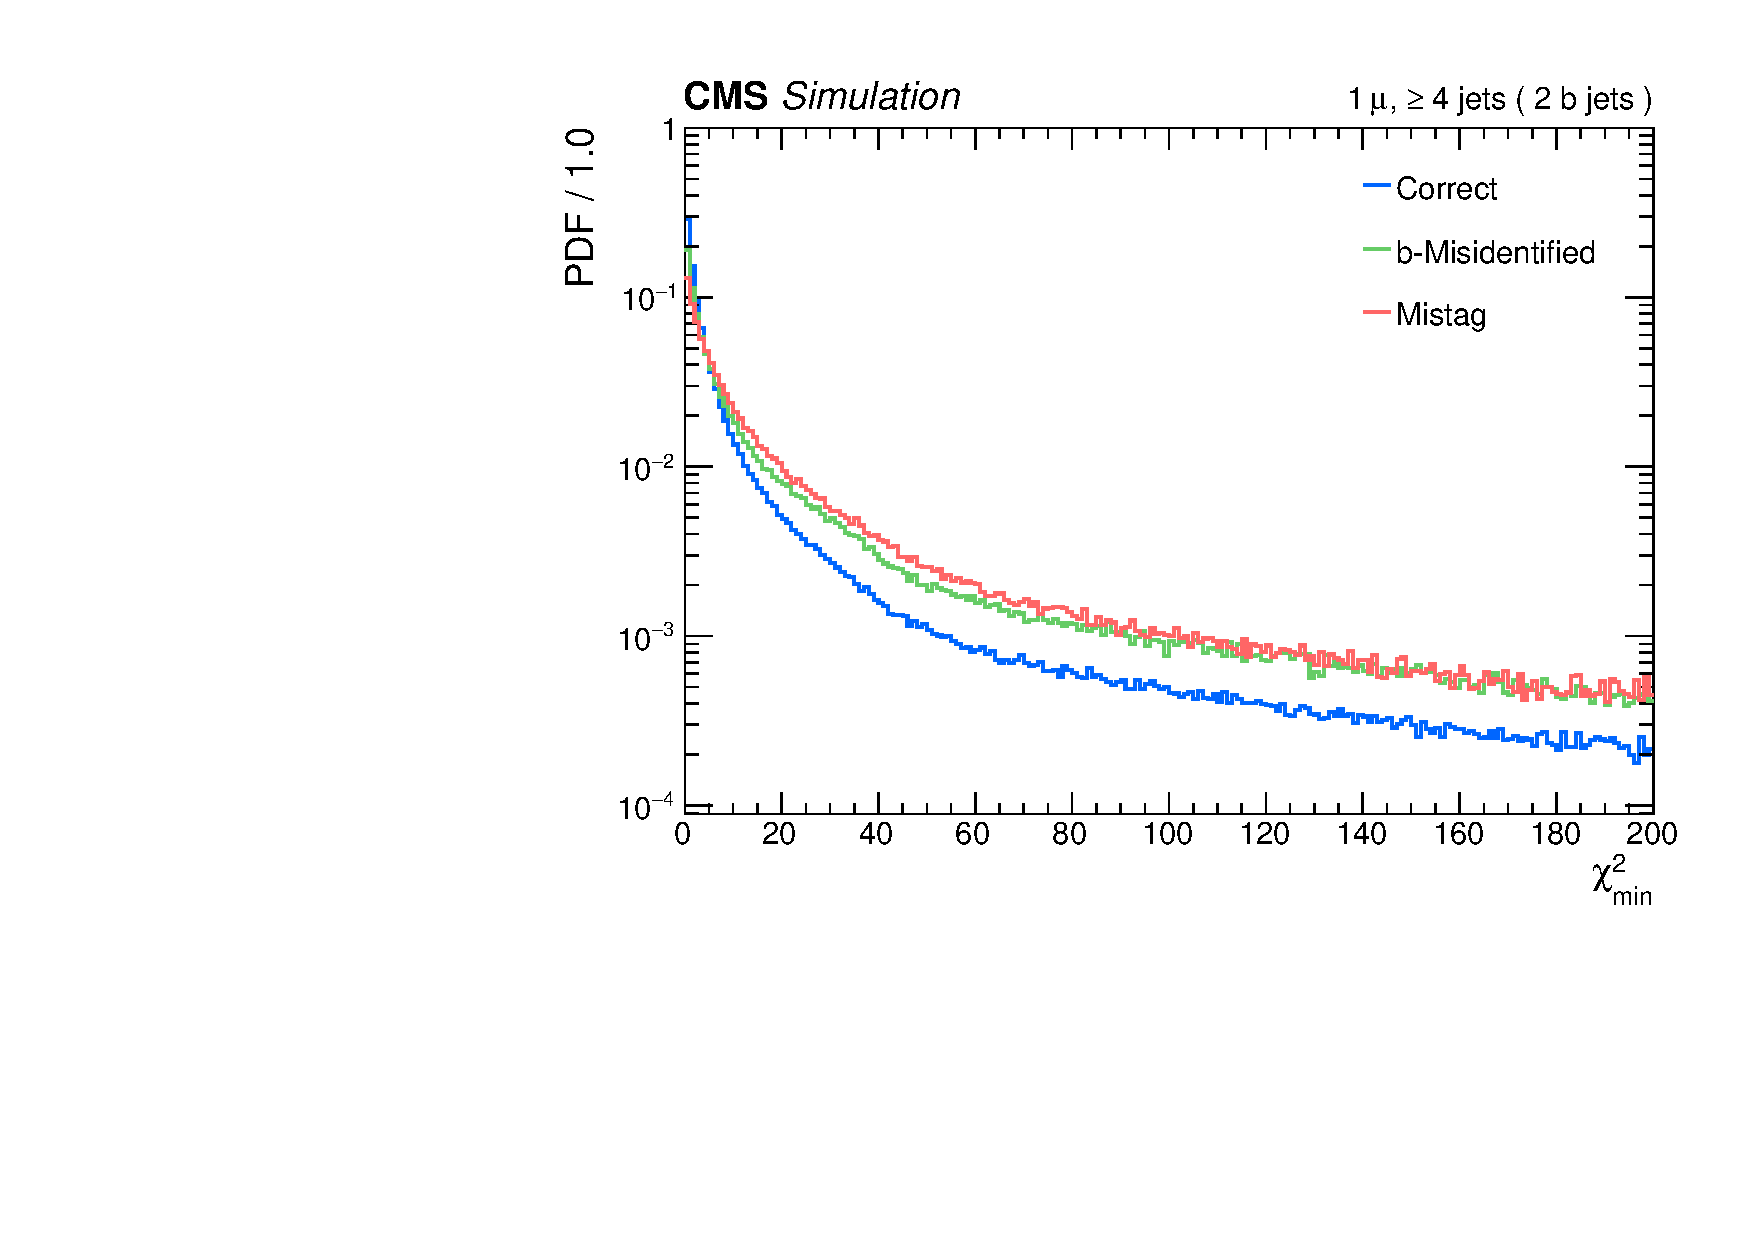
\includegraphics[width=0.45\textwidth]{figure/bbSep_17_mu_Rate_PDF_bbSep.pdf}
    \includegraphics[width=0.45\textwidth]{figure/bbSep_18_el_Rate_PDF_bbSep.pdf}
    \includegraphics[width=0.45\textwidth]{figure/bbSep_18_mu_Rate_PDF_bbSep.pdf}
    \caption[The fraction of different event types in the minimum \chisq distribution.]
    {
        The fraction of different event types in the minimum \chisq distribution in electron channel (left) and muon channel (right) for 2016 (top), 2017 (middle), and 2018 (bottom) samples.
    }
    \label{fig:bbsep_rate}
\end{figure}

\begin{figure}[p]
    \centering
    \includegraphics[width=0.45\textwidth]{figure/bbSep_16_el_Chi2_uppercut_bbSep.pdf}
    \includegraphics[width=0.45\textwidth]{figure/bbSep_16_mu_Chi2_uppercut_bbSep.pdf}
    \includegraphics[width=0.45\textwidth]{figure/bbSep_17_el_Chi2_uppercut_bbSep.pdf}
    \includegraphics[width=0.45\textwidth]{figure/bbSep_17_mu_Chi2_uppercut_bbSep.pdf}
    \includegraphics[width=0.45\textwidth]{figure/bbSep_18_el_Chi2_uppercut_bbSep.pdf}
    \includegraphics[width=0.45\textwidth]{figure/bbSep_18_mu_Chi2_uppercut_bbSep.pdf}
    \caption[The fraction of different event types in the distribution of the upper bound on minimum \chisq.]
    {
        The fraction of different event types in the distribution of upper bound on \chisq in electron channel (left) and muon channel (right) for 2016 (top), 2017 (middle), and 2018 (bottom) samples.
        The red dotted line shows the used uppeer bound in this analysis.
    }
    \label{fig:bbsep_uppercut}
\end{figure}

\begin{figure}[p]
    \centering
    \includegraphics[width=0.45\textwidth]{figure/bbSep_16_el_Optimisation_chi2_20_bbSep.pdf}
    \includegraphics[width=0.45\textwidth]{figure/bbSep_16_mu_Optimisation_chi2_20_bbSep.pdf}
    \includegraphics[width=0.45\textwidth]{figure/bbSep_17_el_Optimisation_chi2_20_bbSep.pdf}
    \includegraphics[width=0.45\textwidth]{figure/bbSep_17_mu_Optimisation_chi2_20_bbSep.pdf}
    \includegraphics[width=0.45\textwidth]{figure/bbSep_18_el_Optimisation_chi2_20_bbSep.pdf}
    \includegraphics[width=0.45\textwidth]{figure/bbSep_18_mu_Optimisation_chi2_20_bbSep.pdf}
    \caption[The \Mlb distribution of different event types.]
    {
        The \Mlb distribution of different event type in electron channel (left) and muon channel (right) for 2016 (top), 2017 (middle), and 2018 (bottom) samples.
    }
    \label{fig:opt_lept}
\end{figure}

\begin{figure}[p]
    \centering
    \includegraphics[width=0.45\textwidth]{figure/bbSep_16_el_OptCut_chi2_20_bbSep.pdf}
    \includegraphics[width=0.45\textwidth]{figure/bbSep_16_mu_OptCut_chi2_20_bbSep.pdf}
    \includegraphics[width=0.45\textwidth]{figure/bbSep_17_el_OptCut_chi2_20_bbSep.pdf}
    \includegraphics[width=0.45\textwidth]{figure/bbSep_17_mu_OptCut_chi2_20_bbSep.pdf}
    \includegraphics[width=0.45\textwidth]{figure/bbSep_18_el_OptCut_chi2_20_bbSep.pdf}
    \includegraphics[width=0.45\textwidth]{figure/bbSep_18_mu_OptCut_chi2_20_bbSep.pdf}
    \caption[The fraction of each event type in \Mlb distribution.]
    {
        The fraction of each event type in \Mlb distribution with the event efficiency in electron channel (left) and muon channel (right) for 2016 (top), 2017 (middle), and 2018 (bottom) samples.
        The red dotted line shows the used uppeer bound in this analysis.
    }
    \label{fig:opt_cut}
\end{figure}

\begin{figure}
    \centering
    \includegraphics[width=0.4\textwidth]{figure/Figure_001-a.pdf}
    \includegraphics[width=0.4\textwidth]{figure/Figure_001-b.pdf}
    \includegraphics[width=0.4\textwidth]{figure/Figure_001-c.pdf}
    \includegraphics[width=0.4\textwidth]{figure/Figure_001-d.pdf}
    \caption[Distributions of the CP observables for electron events in the signal region.]
    {
        Distributions of the CP observables \Othree (upper left), \Osix (upper right), \Otwelve (lower left), and \Ofourteen (lower right), normalized with respect to \Mtcub, from data (points) and from the various sources in simulation (colored histograms) for electron events in the signal region.
        The solid-blue line shows the CEDM simulated signal normalized to the data with the CP-odd parameter $\dtG = +3$.
        The vertical bars on the data points indicate the statistical uncertainties in the data, and the hatched bands show the quadrature sum of the statistical and systematic uncertainties in the simulation.
        The lower two panels display the ratio of the data to the sum of the MC predictions and the ratio of the CEDM to the SM predictions for $\dtG = +3$ (dark-blue lines) and $-3$ (red lines).
    }
    \label{fig:el_obs_dist}
\end{figure}

\begin{figure}
    \centering
    \includegraphics[width=0.4\textwidth]{figure/Figure_002-a.pdf}
    \includegraphics[width=0.4\textwidth]{figure/Figure_002-b.pdf}
    \includegraphics[width=0.4\textwidth]{figure/Figure_002-c.pdf}
    \includegraphics[width=0.4\textwidth]{figure/Figure_002-d.pdf}
    \caption[Distributions of the CP observables for muon events in the signal region.]
    {
        Distributions of the CP observables \Othree (upper left), \Osix (upper right), \Otwelve (lower left), and \Ofourteen (lower right), normalized with respect to \Mtcub, from data (points) and from the various sources in simulation (colored histograms) for muon events in the signal region.
        The solid-blue line shows the CEDM simulated signal normalized to the data with the CP-odd parameter $\dtG = +3$.
        The vertical bars on the data points indicate the statistical uncertainties in the data, and the hatched bands show the quadrature sum of the statistical and systematic uncertainties in the simulation.
        The lower two panels display the ratio of the data to the sum of the MC predictions and the ratio of the CEDM to the SM predictions for $\dtG = +3$ (dark-blue lines) and $-3$ (red lines).
    }
    \label{fig:mu_obs_dist}
\end{figure}

\begin{table}
    \caption[The predicted \ttbar signal and background contributions to the signal events.]
    {
        The predicted \ttbar signal and background contributions to the signal events from simulation for the electron and muon channels.
    }
    \label{tab:signal_region_expected_percentage}
    \centering\renewcommand\arraystretch{1.2}
    \begin{tabular}{ccc}
        Process & Electron channel (\%) & Muon channel (\%) \\
        \hline
        \ttbar in lepton+jets & 89.9 & 89.5\\
        \ttbar in dilepton+jets & 5.5 & 5.5\\
        \ttbar multijet & 0.1 & 0.1\\
        Single \PQt & 2.9 & 2.9\\
        \Wjets & 1.0 & 1.1\\
        DY+jets & 0.4 & 0.2\\
        QCD multijet & 0.2 & 0.6\\
        $\PZ\PZ$ / $\PW\PW$ / $\PW\PZ$ & 0.1 & 0.1\\
    \end{tabular}
\end{table}

Background events can induce spurious measurements of the asymmetries, so a sample of background-enriched data events is used to check for such effects.
In order to enhance the fraction of background events and minimize the contribution from \ttbar, events are required to have no \PQb-tagged jets.
The \PQb jet veto is defined using a weakly restrictive working point of \DeepCSV, corresponding to an 84\% efficiency in identifying \PQb jets and an 11\% misidentification rate for light-flavor quark and gluon jets~\cite{CMS:bjet_eff}.
The isolation requirement in the looser set of selection criteria for leptons is relaxed, so events with additional leptons produced through the decay of a bottom quark can be more highly rejected.
The rest of the selection criteria are the same as used for the signal events.
The object assigned by the $\chisq$ algorithm takes the role of the \PQb jet coming from the hadronically decaying top quark, and the jet closest to the isolated lepton is assigned as the other \PQb jet.
The background-enriched events are expected to be dominated by non-\ttbar processes ($\approx$90\%), including a major contribution from \Wjets.

\chapter{Asymmetries extraction}\label{sec:fitresult}
    \section{Fitting procedure}
    The presence of CPV can manifest itself through a nonzero value of the asymmetry defined as
\begin{linenomath}\begin{equation}\label{eq:counting_method}
    \Acp(\Oi) = \frac{\Npos-\Nneg}{\Npos+\Nneg},\quad i=3,\,6,\,12,\,14.
\end{equation}\end{linenomath}
The CP-violating asymmetries $\Acp(\Oi)$ are expected to vanish in the SM.
However, nonzero CP-violating couplings of the top quark from BSM phenomena can lead to sizable asymmetries.
An anomalous CEDM contribution~\cite{CPVtop:13TeVRef} can be as large as 8 and 0.4\% for $\Acp(\Othree)$ and $\Acp(\Otwelve)$, respectively.

Experimental factors, such as the misreconstruction of the physical objects, can affect the measurements of the asymmetries~\cite{CPVtop:13TeVRef}.
For example, misidentified signal events coming from \ttbar in the dilepton+jets channel can cause spurious asymmetry measurements.
We denote \Acp as the asymmetry that would be measured with an ideal detector and \Acpprime as the measured effective asymmetry, including experimental factors.
An estimate of \Acp can be obtained after correcting the measured asymmetry for instrumental effects.
Given that the SM predicts negligible \Acp in the top quark sector, a nonzero effective \Acpprime would be a strong hint of BSM phenomena.
For this reason, measurements of \Acpprime can be computed using \ttbar events and are the primary results presented in this paper.

Because \ttbar multijet events are highly suppressed by the signal-event requirements, only the \ttbar to lepton+jets and dilepton+jets channels are considered in the \ttbar contribution, with the latter assumed to be background.
The signal and background yields are determined through an extended maximum likelihood fit to the \Mlb distributions in data using simulated-event templates.
The \ttbar template is obtained from simulation, and the background template from the background-enriched events in data.
For each CP observable, the templates are classified according to the sign of the CP observable.
The extended likelihood function is defined as
\begin{linenomath}\begin{equation}\begin{aligned}
    L_{\text{ext}} &= \frac{\re^{-(\numpos+\ratiob \numb)}}{\Numpos!}\prod^{\Numpos}_{i=1} \numpos \fspos(\Mlbi) + \ratiob \numb \fbpos(\Mlbi) \\
    &+ \frac{\re^{-(\numneg+(1-\ratiob) \numb)}}{\Numneg!}\prod^{\Numneg}_{i=1} \numneg \fsneg(\Mlbi) + (1-\ratiob) \numb \fbneg(\Mlbi),
\end{aligned}\end{equation}\end{linenomath}
where \numb, \numpos, and \numneg are the parameters of interest and refer to the yields of background, and \ttbar events with positive and negative CP observable values, respectively; \ratiob refers to the fraction of background events with positive CP observable values obtained from the background template; $\fspos(\Mlb)$, $\fsneg(\Mlb)$, $\fbpos(\Mlb)$, and $\fbneg(\Mlb)$ refer to the probability density functions (pdf) of \Mlb obtained from the \ttbar and background templates according to the sign of the CP observable, respectively; and \Numpos and \Numneg are the number of events according to the sign of the CP observable.
To improve the fit results, the upper bound on \Mlb is relaxed to 500\GeV in the fit in order to include more sideband events.
However, to be consistent with the signal-event requirements, events with $\Mlb > 150\GeV$ are excluded after the fit in determining the final event yields for each CP observable.

Figures~\ref{fig:CR_SR_closure_test16},~\ref{fig:CR_SR_closure_test17},~\ref{fig:CR_SR_closure_test18} show the normalized \Mlb distributions from the signal and background-enriched events for the electron (left) and muon (right) channels.
The upper plots compare the distribution for the background-enriched data events to that from the MC prediction.
Good agreement is observed between the two distributions, showing that the background-enriched events are consistent with being entirely background.
The lower plots display the distributions for the background-enriched events in data and the predicted MC background in the signal-event sample.
The \Mlb distribution of background-enriched events in data is slightly wider than the predicted MC background in signal events.
This difference is taken as one of the systematic uncertainties, as discussed in Section~\ref{sec:uncertainty}.

\begin{figure}
    \centering
    \includegraphics[width=0.45\textwidth]{figure/BGClosureTest_16_el_CR_chi2_20_wobtag.pdf}
    \includegraphics[width=0.45\textwidth]{figure/BGClosureTest_16_mu_CR_chi2_20_wobtag.pdf}
    \includegraphics[width=0.45\textwidth]{figure/BGClosureTest_16_el_SR_chi2_20_wobtag.pdf}
    \includegraphics[width=0.45\textwidth]{figure/BGClosureTest_16_mu_SR_chi2_20_wobtag.pdf}
    \caption[The normalized \Mlb distributions in 2016 samples.]
    {
        The normalized \Mlb distributions for the electron (left) and muon (right) channels in 2016 samples.
        The upper two plots compare the background-enriched distributions from data (solid line) to the MC predictions (dotted-red line).
        The lower two plots give the background-enriched distributions from data (solid line) and the MC predictions for the distributions from the background in the signal events.
    }
    \label{fig:CR_SR_closure_test16}
\end{figure}

\begin{figure}
    \centering
    \includegraphics[width=0.45\textwidth]{figure/BGClosureTest_17_el_CR_chi2_20_wobtag.pdf}
    \includegraphics[width=0.45\textwidth]{figure/BGClosureTest_17_mu_CR_chi2_20_wobtag.pdf}
    \includegraphics[width=0.45\textwidth]{figure/BGClosureTest_17_el_SR_chi2_20_wobtag.pdf}
    \includegraphics[width=0.45\textwidth]{figure/BGClosureTest_17_mu_SR_chi2_20_wobtag.pdf}
    \caption[The normalized \Mlb distributions in 2017 samples.]
    {
        The normalized \Mlb distributions for the electron (left) and muon (right) channels in 2017 samples.
        The upper two plots compare the background-enriched distributions from data (solid line) to the MC predictions (dotted-red line).
        The lower two plots give the background-enriched distributions from data (solid line) and the MC predictions for the distributions from the background in the signal events.
    }
    \label{fig:CR_SR_closure_test17}
\end{figure}

\begin{figure}
    \centering
    \includegraphics[width=0.45\textwidth]{figure/BGClosureTest_18_el_CR_chi2_20_wobtag.pdf}
    \includegraphics[width=0.45\textwidth]{figure/BGClosureTest_18_mu_CR_chi2_20_wobtag.pdf}
    \includegraphics[width=0.45\textwidth]{figure/BGClosureTest_18_el_SR_chi2_20_wobtag.pdf}
    \includegraphics[width=0.45\textwidth]{figure/BGClosureTest_18_mu_SR_chi2_20_wobtag.pdf}
    \caption[The normalized \Mlb distributions in 2018 samples.]
    {
        The normalized \Mlb distributions for the electron (left) and muon (right) channels in 2018 samples.
        The upper two plots compare the background-enriched distributions from data (solid line) to the MC predictions (dotted-red line).
        The lower two plots give the background-enriched distributions from data (solid line) and the MC predictions for the distributions from the background in the signal events.
    }
    \label{fig:CR_SR_closure_test18}
\end{figure}

The \Mlb distributions in data per year are shown in Figs.~\ref{fig:fitting_results_16_el},~\ref{fig:fitting_results_16_mu},~\ref{fig:fitting_results_17_el},~\ref{fig:fitting_results_17_mu},~\ref{fig:fitting_results_18_el},~\ref{fig:fitting_results_18_mu} along with the results of the fit.
The combined measured numbers of \ttbar signal and background events in the electron and muon channels from the fits, and the corresponding \ttbar purities, are presented in Table~\ref{tab:fitting_purity}.
The final \Acpprime measurements can then be computed using the event-counting method of Eq.~\eqref{eq:counting_method}.
\begin{figure}
    \centering
    \includegraphics[width=0.4\textwidth]{figure/FitResult_16_el_lep_tmass_obs3_p_chi2_20.pdf}
    \includegraphics[width=0.4\textwidth]{figure/FitResult_16_el_lep_tmass_obs3_n_chi2_20.pdf}
    \includegraphics[width=0.4\textwidth]{figure/FitResult_16_el_lep_tmass_obs6_p_chi2_20.pdf}
    \includegraphics[width=0.4\textwidth]{figure/FitResult_16_el_lep_tmass_obs6_n_chi2_20.pdf}
    \includegraphics[width=0.4\textwidth]{figure/FitResult_16_el_lep_tmass_obs12_p_chi2_20.pdf}
    \includegraphics[width=0.4\textwidth]{figure/FitResult_16_el_lep_tmass_obs12_n_chi2_20.pdf}
    \includegraphics[width=0.4\textwidth]{figure/FitResult_16_el_lep_tmass_obs14_p_chi2_20.pdf}
    \includegraphics[width=0.4\textwidth]{figure/FitResult_16_el_lep_tmass_obs14_n_chi2_20.pdf}
    \caption[The \Mlb invariant mass distributions in electron channel from 2016 data.]
    {
        The \Mlb invariant mass distributions in the positive (left) and negative (right) observable value region in electron channel from 2016 data (points).
        The results of the fit to the \ttbar and background templates are shown by the red and green histograms, respectively.
        The vertical bars on the data points in the upper panels indicate the statistical uncertainties in the data and the hatched bands show the combined statistical and systematic uncertainties in the simulation.
        The lower panels give the ratio of the data to the sum of the fitted MC predictions.
        The blue bands represent the systematic uncertainties in the expected yield in the simulation for all sources of systematic uncertainty (Section~\ref{sec:uncertainty}).
    }
    \label{fig:fitting_results_16_el}
\end{figure}

\begin{figure}
    \centering
    \includegraphics[width=0.4\textwidth]{figure/FitResult_16_mu_lep_tmass_obs3_p_chi2_20.pdf}
    \includegraphics[width=0.4\textwidth]{figure/FitResult_16_mu_lep_tmass_obs3_n_chi2_20.pdf}
    \includegraphics[width=0.4\textwidth]{figure/FitResult_16_mu_lep_tmass_obs6_p_chi2_20.pdf}
    \includegraphics[width=0.4\textwidth]{figure/FitResult_16_mu_lep_tmass_obs6_n_chi2_20.pdf}
    \includegraphics[width=0.4\textwidth]{figure/FitResult_16_mu_lep_tmass_obs12_p_chi2_20.pdf}
    \includegraphics[width=0.4\textwidth]{figure/FitResult_16_mu_lep_tmass_obs12_n_chi2_20.pdf}
    \includegraphics[width=0.4\textwidth]{figure/FitResult_16_mu_lep_tmass_obs14_p_chi2_20.pdf}
    \includegraphics[width=0.4\textwidth]{figure/FitResult_16_mu_lep_tmass_obs14_n_chi2_20.pdf}
    \caption[The \Mlb invariant mass distributions in muon channel from 2016 data.]
    {
        The \Mlb invariant mass distributions in the positive (left) and negative (right) observable value region in muon channel from 2016 data (points).
        The results of the fit to the \ttbar and background templates are shown by the red and green histograms, respectively.
        The vertical bars on the data points in the upper panels indicate the statistical uncertainties in the data and the hatched bands show the combined statistical and systematic uncertainties in the simulation.
        The lower panels give the ratio of the data to the sum of the fitted MC predictions.
        The blue bands represent the systematic uncertainties in the expected yield in the simulation for all sources of systematic uncertainty (Section~\ref{sec:uncertainty}).
    }
    \label{fig:fitting_results_16_mu}
\end{figure}
\begin{figure}
    \centering
    \includegraphics[width=0.4\textwidth]{figure/FitResult_17_el_lep_tmass_obs3_p_chi2_20.pdf}
    \includegraphics[width=0.4\textwidth]{figure/FitResult_17_el_lep_tmass_obs3_n_chi2_20.pdf}
    \includegraphics[width=0.4\textwidth]{figure/FitResult_17_el_lep_tmass_obs6_p_chi2_20.pdf}
    \includegraphics[width=0.4\textwidth]{figure/FitResult_17_el_lep_tmass_obs6_n_chi2_20.pdf}
    \includegraphics[width=0.4\textwidth]{figure/FitResult_17_el_lep_tmass_obs12_p_chi2_20.pdf}
    \includegraphics[width=0.4\textwidth]{figure/FitResult_17_el_lep_tmass_obs12_n_chi2_20.pdf}
    \includegraphics[width=0.4\textwidth]{figure/FitResult_17_el_lep_tmass_obs14_p_chi2_20.pdf}
    \includegraphics[width=0.4\textwidth]{figure/FitResult_17_el_lep_tmass_obs14_n_chi2_20.pdf}
    \caption[The \Mlb invariant mass distributions in electron channel from 2017 data.]
    {
        The \Mlb invariant mass distributions in the positive (left) and negative (right) observable value region in electron channel from 2017 data (points).
        The results of the fit to the \ttbar and background templates are shown by the red and green histograms, respectively.
        The vertical bars on the data points in the upper panels indicate the statistical uncertainties in the data and the hatched bands show the combined statistical and systematic uncertainties in the simulation.
        The lower panels give the ratio of the data to the sum of the fitted MC predictions.
        The blue bands represent the systematic uncertainties in the expected yield in the simulation for all sources of systematic uncertainty (Section~\ref{sec:uncertainty}).
    }
    \label{fig:fitting_results_17_el}
\end{figure}
\begin{figure}
    \centering
    \includegraphics[width=0.4\textwidth]{figure/FitResult_17_mu_lep_tmass_obs3_p_chi2_20.pdf}
    \includegraphics[width=0.4\textwidth]{figure/FitResult_17_mu_lep_tmass_obs3_n_chi2_20.pdf}
    \includegraphics[width=0.4\textwidth]{figure/FitResult_17_mu_lep_tmass_obs6_p_chi2_20.pdf}
    \includegraphics[width=0.4\textwidth]{figure/FitResult_17_mu_lep_tmass_obs6_n_chi2_20.pdf}
    \includegraphics[width=0.4\textwidth]{figure/FitResult_17_mu_lep_tmass_obs12_p_chi2_20.pdf}
    \includegraphics[width=0.4\textwidth]{figure/FitResult_17_mu_lep_tmass_obs12_n_chi2_20.pdf}
    \includegraphics[width=0.4\textwidth]{figure/FitResult_17_mu_lep_tmass_obs14_p_chi2_20.pdf}
    \includegraphics[width=0.4\textwidth]{figure/FitResult_17_mu_lep_tmass_obs14_n_chi2_20.pdf}
    \caption[The \Mlb invariant mass distributions in muon channel from 2017 data.]
    {
        The \Mlb invariant mass distributions in the positive (left) and negative (right) observable value region in muon channel from 2017 data (points).
        The results of the fit to the \ttbar and background templates are shown by the red and green histograms, respectively.
        The vertical bars on the data points in the upper panels indicate the statistical uncertainties in the data and the hatched bands show the combined statistical and systematic uncertainties in the simulation.
        The lower panels give the ratio of the data to the sum of the fitted MC predictions.
        The blue bands represent the systematic uncertainties in the expected yield in the simulation for all sources of systematic uncertainty (Section~\ref{sec:uncertainty}).
    }
    \label{fig:fitting_results_17_mu}
\end{figure}
\begin{figure}
    \centering
    \includegraphics[width=0.4\textwidth]{figure/FitResult_18_el_lep_tmass_obs3_p_chi2_20.pdf}
    \includegraphics[width=0.4\textwidth]{figure/FitResult_18_el_lep_tmass_obs3_n_chi2_20.pdf}
    \includegraphics[width=0.4\textwidth]{figure/FitResult_18_el_lep_tmass_obs6_p_chi2_20.pdf}
    \includegraphics[width=0.4\textwidth]{figure/FitResult_18_el_lep_tmass_obs6_n_chi2_20.pdf}
    \includegraphics[width=0.4\textwidth]{figure/FitResult_18_el_lep_tmass_obs12_p_chi2_20.pdf}
    \includegraphics[width=0.4\textwidth]{figure/FitResult_18_el_lep_tmass_obs12_n_chi2_20.pdf}
    \includegraphics[width=0.4\textwidth]{figure/FitResult_18_el_lep_tmass_obs14_p_chi2_20.pdf}
    \includegraphics[width=0.4\textwidth]{figure/FitResult_18_el_lep_tmass_obs14_n_chi2_20.pdf}
    \caption[The \Mlb invariant mass distributions in electron channel from 2018 data.]
    {
        The \Mlb invariant mass distributions in the positive (left) and negative (right) observable value region in electron channel from 2018 data (points).
        The results of the fit to the \ttbar and background templates are shown by the red and green histograms, respectively.
        The vertical bars on the data points in the upper panels indicate the statistical uncertainties in the data and the hatched bands show the combined statistical and systematic uncertainties in the simulation.
        The lower panels give the ratio of the data to the sum of the fitted MC predictions.
        The blue bands represent the systematic uncertainties in the expected yield in the simulation for all sources of systematic uncertainty (Section~\ref{sec:uncertainty}).
    }
    \label{fig:fitting_results_18_el}
\end{figure}
\begin{figure}
    \centering
    \includegraphics[width=0.4\textwidth]{figure/FitResult_18_mu_lep_tmass_obs3_p_chi2_20.pdf}
    \includegraphics[width=0.4\textwidth]{figure/FitResult_18_mu_lep_tmass_obs3_n_chi2_20.pdf}
    \includegraphics[width=0.4\textwidth]{figure/FitResult_18_mu_lep_tmass_obs6_p_chi2_20.pdf}
    \includegraphics[width=0.4\textwidth]{figure/FitResult_18_mu_lep_tmass_obs6_n_chi2_20.pdf}
    \includegraphics[width=0.4\textwidth]{figure/FitResult_18_mu_lep_tmass_obs12_p_chi2_20.pdf}
    \includegraphics[width=0.4\textwidth]{figure/FitResult_18_mu_lep_tmass_obs12_n_chi2_20.pdf}
    \includegraphics[width=0.4\textwidth]{figure/FitResult_18_mu_lep_tmass_obs14_p_chi2_20.pdf}
    \includegraphics[width=0.4\textwidth]{figure/FitResult_18_mu_lep_tmass_obs14_n_chi2_20.pdf}
    \caption[The \Mlb invariant mass distributions in muon channel from 2018 data.]
    {
        The \Mlb invariant mass distributions in the positive (left) and negative (right) observable value region in muon channel from 2018 data (points).
        The results of the fit to the \ttbar and background templates are shown by the red and green histograms, respectively.
        The vertical bars on the data points in the upper panels indicate the statistical uncertainties in the data and the hatched bands show the combined statistical and systematic uncertainties in the simulation.
        The lower panels give the ratio of the data to the sum of the fitted MC predictions.
        The blue bands represent the systematic uncertainties in the expected yield in the simulation for all sources of systematic uncertainty (Section~\ref{sec:uncertainty}).
    }
    \label{fig:fitting_results_18_mu}
\end{figure}

\begin{table}
    \caption[The fitted number of \ttbar signal and \ttbar background events and other background events.]
    {
        The fitted number of \ttbar signal and \ttbar background events (fitted \ttbar) and other background events (fitted background) in the electron and muon channels, along with the \ttbar purities.
        Although the fit is performed for $\Mlb < 500\GeV$, the event yields are given for $\Mlb < 150\GeV$.
        The uncertainties shown are statistical only.
    }
    \label{tab:fitting_purity}
    \centering\renewcommand\arraystretch{1.2}
    \begin{tabular}{ccc}
        & Electron channel & Muon channel\\
        \hline
        Fitted \ttbar & $604\,700 \pm 1200$ & $1\,062\,600 \pm 1500$\\
        Fitted background & $34\,030 \pm 480$ & $58\,490 \pm 820$\\
        Fitted fraction of \ttbar (\%) & $94.7 \pm 0.1$ & $94.8 \pm 0.1$ \\
    \end{tabular}
\end{table}




    \section{Experimental sensitivity}
    The sensitivity of the asymmetry measurement can be diluted due to detector and reconstruction effects, which can be parametrized through a dilution factor (\dilution).
The \Acpprime and \Acp values are related through \dilution, applied as a multiplicative correction $\Acpprime = \dilution \Acp$~\cite{CPVtop:13TeVRef}.
The dilution factor can be defined as
\begin{linenomath}\begin{equation}
    \dilution = \epsc - \epsw,
\end{equation}\end{linenomath}
where \epsc is the fraction of events where the measured CP observable has the correct sign, and \epsw is the fraction with the wrong sign.
Events are classified into the correct-sign (wrong-sign) type when the sign of the CP observable at the reconstruction level agrees with (differs from) that at the \POWHEG generator level.

The value of \dilution depends on the final-state objects used to form each CP observable.
In contrast to \Otwelve and \Ofourteen, it is necessary for \Othree and \Osix to distinguish the charges of the \PQb quarks by using the sign of the lepton charge, and therefore they tend to have a lower fraction of correct-sign events and smaller values of \dilution.
The value of \dilution can also be affected by possible contributions of BSM processes, because the CP observables are reconstructed using kinematic features of the final-state objects.
The model-dependency in the dilution factor of each observable is studied using SM simulated \ttbar samples and CEDM model simulated \ttbar samples.
Figure~\ref{fig:DF_CEDM_SM} shows that the differences between different models are negligible and consistent with unity within one standard deviation in the low \dtG region.
The values of \dilution determined from the SM simulations are given in Table~\ref{tab:dilution_factor}, along with their systematic uncertainties described in Section~\ref{sec:uncertainty}.

\begin{figure}
    \centering
    \includegraphics[width=0.45\textwidth]{figure/Ratio_17_co_DF_Obs3_chi2_20_opt_150.pdf}
    \includegraphics[width=0.45\textwidth]{figure/Ratio_17_co_DF_Obs6_chi2_20_opt_150.pdf}
    \includegraphics[width=0.45\textwidth]{figure/Ratio_17_co_DF_Obs12_chi2_20_opt_150.pdf}
    \includegraphics[width=0.45\textwidth]{figure/Ratio_17_co_DF_Obs14_chi2_20_opt_150.pdf}
    \caption[Model dependency for the dilution factor for each observable.]
    {
        Model dependency for the dilution factor for each observable. 
        The points show the ratio between the value obtained by re-weigthing events according to different CEDM models with the baseline results obtained in the SM simulation.
        It should be noticed that, although all the points are correlated, the deviations from unity are much smaller than the statistical error represented by the error bars in the low \dtG region.
    }
    \label{fig:DF_CEDM_SM}
\end{figure}

\begin{table}[!h]
    \caption[The dilution factor \dilution for each CP observable.]
    {
        The dilution factor \dilution determined from simulation and its systematic uncertainty for each CP observable.
        The statistical uncertainty is negligible compared to the systematic uncertainty.
    }
    \label{tab:dilution_factor}
    \centering\renewcommand\arraystretch{1.4}
    \begin{tabular}{cc}
        CP observable & Dilution factor \dilution \\
        \hline
        \Othree  & $0.46\,^{+0.01}_{-0.02}$\\
        \Osix  & $0.44\,^{+0.01}_{-0.02}$\\
        \Otwelve & $0.74\,^{+0.01}_{-0.02}$\\
        \Ofourteen & $0.60\,^{+0.01}_{-0.01}$\\
    \end{tabular}
\end{table}

In order to better understand the measured \dilution values, the lepton+jets and dilepton+jets events in the simulated \ttbar samples are reweighted at the generator level to produce various pseudo-asymmetry values.
The SM simulated \ttbar events can be reweighted as 

\begin{align}
    w^{+}_i &= 1 + A_{CP}(O_i) \\
    w^{-}_i &= 1 - A_{CP}(O_i) 
\end{align}

where \Acp$(O_i)$ is the input artificial \Acp value for each observable, $w^{+(-)}_i$ is a weight for events with positive (negative) value of $O_i$ at generator level.
For example, if we want to have $+5\%$ \Acp value in \Othree, the event weight for $w^{+}_{3}$ will be $1.05$ and $w^{-}_{3}$ will be $0.95$. 
As shown in Fig.~\ref{fig:check_dilution_factor}, the CP-violating asymmetries \Acp (diamond points) are then obtained by dividing the effective asymmetries \Acpprime (circular points) by the corresponding dilution factor determined from simulation.
Fitting the \Acpprime and \Acp values to linear functions of the generator-level pseudo-asymmetry values results in the red-dotted and blue-solid lines shown in Fig.~\ref{fig:check_dilution_factor}, respectively.
All the fits have good \chisq values, and the slopes and $y$ intercepts of the fitted lines to \Acp are consistent with 1.0 and 0.0, respectively.

\begin{figure}[h!]
    \centering
    \includegraphics[width=0.45\textwidth]{figure/Figure_005-a.pdf}
    \includegraphics[width=0.45\textwidth]{figure/Figure_005-b.pdf}
    \includegraphics[width=0.45\textwidth]{figure/Figure_005-c.pdf}
    \includegraphics[width=0.45\textwidth]{figure/Figure_005-d.pdf}
    \caption[The measured CP-violating asymmetries as a function of the pseudo-asymmetry.]
    {
        The measured CP-violating asymmetries in simulation as a function of the generator-level pseudo-asymmetry for the CP observables \Othree (upper left), \Osix (upper right), \Otwelve (lower left), and \Ofourteen (lower right).
        The red circles and blue diamonds give the \Acpprime and \Acp values, respectively, with the red-dotted and blue-solid lines showing the results of linear fits to those corresponding values.
        The \Acp value is obtained by dividing the \Acpprime value by the dilution factor determined from simulation for that CP observable.
        The statistical uncertainties in the \Acpprime values are smaller than the markers.
    }
    \label{fig:check_dilution_factor}
\end{figure}

\chapter{Systematic uncertainties}\label{sec:uncertainty}
    The sources of systematic uncertainty considered in this paper are presented below in the following order: intrinsic detector bias, other experimental uncertainties, and theoretical uncertainties.
The systematic effects are expected to contribute similarly to the positive and negative regions of each CP observable, thereby largely canceling in the ratio shown in Eq.~\eqref{eq:counting_method}, used to measure the CP asymmetries.

    \section{Detector and reconstruction effects}
    The CP-violating asymmetries can arise due to both couplings from BSM processes and detector and reconstruction effects.
The previous study at \oldTeV used background-enriched data to study the detector bias~\cite{CPVtop:CMSresult}.
The precision in the modeling of the resulting CP-violating asymmetries caused by detector and reconstruction effects may be improved by studying signal events, and therefore an event-mixing method is used to evaluate the possible bias resulting in a nonzero value of \Acpprime.
The method using background-enriched data is also introduced here along with the event-mixing method.

\subsection{Background-enriched method}
Based on the assumption of no asymmetry in the background events, a sample of background-enriched data events can be used to estimate the detector bias.
This sample is selected by rejecting events with b-tagged jets and is expected to be dominated by background events.
It contains a sufficiently large number of events to perform statistically significant cross checks.
However, the fraction of \ttbar event is up to about $8\%$ in this sample, which may contaminate the measured results.
Secondly, the kinematics of backgrounds may differ from top pair events, and assumption of no asymmetry in background process has to be introduced.
Therefore, in this analysis, we determine to measure detector and reconstruction bias using \ttbar events.
We believe there is no better control sample than \ttbar itself, and the statistics is much higher as well.

\subsection{Event-mixing method}
The event-mixing method is aimed to eliminate the asymmetries from new physics in the sample, and then the asymmetries coming from detector and reconstruction effects can be directly measured. 
This method is performed by mixing the four-momentum information of the \PQb-tagged jet from the hadronically decaying top quark and the highest \PT light-flavor jet among the events.
A total of 1000 mixed data sets are produced by applying the event-mixing method to the data in the signal events to eliminate possible effects from any BSM coupling.
For the $i^{\text{th}}$ mixed data set, the corresponding four-momentum information of the $j^{\text{th}}$ event is passed circularly to the $(j+i)^{\text{th}}$ event.
The resulting sets of asymmetries are independent of the physical processes involved in the signal and background events and represent only the bias from the detector and reconstruction effects.
Separate measurements are performed for each CP observable, year of data taking, and lepton flavor.
The resulting mean values of \Acpprime are presented in Table~\ref{tab:detector_bias} and show no statistically significant detector or reconstruction bias for either lepton flavor.

The correlation between different mixed samples has been studied with parton-level SM simulated \ttbar samples using \MADGRAPH.
A total of 1001 sets of data with 200k events are produced.
The event-mixing method is applied to the first set of data to produce 1000 sets of mixed samples.
The resulting \Acpprime distribution of the mixed samples and the remaining 1000 sets of data are displayed in Fig.~\ref{fig:correlation_study}.
The results show no obvious correlation between those distribution and thus the correlation between mixed samples is neglected in the following process.

This method is tested with \ttbar events with artificial \Acpprime and \ttbar events with intrinsic detector bias.
The \ttbar events with artificial \Acpprime can be produced by randomly picking up $10\%$ more events with positive \Acp in SM simulated \ttbar sample at generator level.
The results are presented in Fig.~\ref{fig:artificial_acp} with around $2$ to $4\%$ artificial \Acpprime.
The resulting mean values of \Acpprime after applying the event-mixing method to \ttbar events with artificial \Acpprime are presented in Figs.~\ref{fig:16_exchanging_simulation_acp},~\ref{fig:17_exchanging_simulation_acp},~\ref{fig:18_exchanging_simulation_acp}.
The results show no statistically significant asymmetries for either lepton flavor.
The \ttbar events with intrinsic detector bias is produced by lowering the detector resolution in SM simulated \ttbar samples.
The values of $\theta$ and $\phi$ are assigned to the same value, for example, the $\theta$ and $\phi$ of b-tagging jets are assigned to $0.5\pi$ and $0.8\pi$ if their original angle is between $0.5\pi - 0.8\pi$ and $0 - 0.67\pi$, respectively.
The test is performed with the least sensitive observable \Otwelve, and the results in Fig~\ref{fig:closure_test_acp} show that the event-mixing method can retain the intrinsic bias.

\subsection{Asymmetries in simulated samples}
The expected values of \Acpprime are supposed to be zero in SM simulated \ttbar and background events.
However, the \Acpprime might be biased due to the imperfection during the simulation process.

The \Acpprime value for SM simulated \ttbar are shown with only statistical uncertainties in Fig~\ref{fig:simulated_signal_acp}, and the \Acpprime values of simulated backgrounds are shown in Fig~\ref{fig:simulated_background_acp}.
Both results show no significant bias  within two standard deviation after combining both the electron and muon channel which is consistent with the prediction from standard model.

\begin{figure}
    \centering
    \includegraphics[width=0.45\textwidth]{figure/SimAcp_16_el_ttbar_chi2_20_opt_150.pdf}
    \includegraphics[width=0.45\textwidth]{figure/SimAcp_16_mu_ttbar_chi2_20_opt_150.pdf}
    \includegraphics[width=0.45\textwidth]{figure/SimAcp_17_el_ttbar_chi2_20_opt_150.pdf}
    \includegraphics[width=0.45\textwidth]{figure/SimAcp_17_mu_ttbar_chi2_20_opt_150.pdf}
    \includegraphics[width=0.45\textwidth]{figure/SimAcp_18_el_ttbar_chi2_20_opt_150.pdf}
    \includegraphics[width=0.45\textwidth]{figure/SimAcp_18_mu_ttbar_chi2_20_opt_150.pdf}
    \caption[The \Acpprime for each observable in SM simulated semileptonic and dileptonic \ttbar events.]
    {
        The \Acpprime for each observable in SM simulated semileptonic and dileptonic \ttbar events for both channels.
        The green(yellow) band is the statistical uncertainty with $1\sigma$($2\sigma$) of the standard deviation(s).
        The electron channel is on the left, and the muon channel is on the right.
        Plots are for 2016, 2017 and 2018 from the top to the bottom separately.
    }
    \label{fig:simulated_signal_acp}
\end{figure}

\begin{figure}
    \centering
    \includegraphics[width=0.45\textwidth]{figure/SimAcp_16_el_background_chi2_20_opt_150.pdf}
    \includegraphics[width=0.45\textwidth]{figure/SimAcp_16_mu_background_chi2_20_opt_150.pdf}
    \includegraphics[width=0.45\textwidth]{figure/SimAcp_17_el_background_chi2_20_opt_150.pdf}
    \includegraphics[width=0.45\textwidth]{figure/SimAcp_17_mu_background_chi2_20_opt_150.pdf}
    \includegraphics[width=0.45\textwidth]{figure/SimAcp_18_el_background_chi2_20_opt_150.pdf}
    \includegraphics[width=0.45\textwidth]{figure/SimAcp_18_mu_background_chi2_20_opt_150.pdf}
    \caption[The \Acpprime for each observable in simulated background events.]
    {
        The \Acpprime for each observable in simulated background events in for both channels.
        The green(yellow) band is the statistical uncertainty with $1\sigma$($2\sigma$) of the standard deviation(s).
        The electron channel is on the left, and the muon channel is on the right.
        Plots are for 2016, 2017 and 2018 from the top to the bottom separately.
    }
    \label{fig:simulated_background_acp}
\end{figure}

\begin{table}
    \caption[The \Acpprime values and their statistical uncertainties in percent for each CP observable.]
    {
        The \Acpprime values and their statistical uncertainties in percent for each CP observable from the electron and muon event-mixing samples and their combination, used to search for detector or reconstruction bias.
    }
    \label{tab:detector_bias}
    \centering\renewcommand\arraystretch{1.2}
    \begin{tabular}{cccc}
        \multicolumn{4}{c}{\Acpprime from event-mixing samples (\%)}\\
        CP observable & \ejets & \mjets & Combined\\
        \hline
        \Othree & $-0.004 \pm 0.004$ & $+0.005 \pm 0.003$ & $+0.003 \pm 0.003$\\
        \Osix & $-0.006 \pm 0.005$ & $+0.003 \pm 0.003$ & $+0.003 \pm 0.003$\\
        \Otwelve & $+0.005 \pm 0.005$ & $-0.001 \pm 0.003$ & $+0.001 \pm 0.002$\\
        \Ofourteen & $-0.008 \pm 0.004$ & $-0.001 \pm 0.003$ & $-0.005 \pm 0.002$\\
    \end{tabular}
\end{table}

\begin{figure}
    \centering
    \includegraphics[width=0.45\textwidth]{figure/SimAcp_RunII_co_obs3.pdf}
    \includegraphics[width=0.45\textwidth]{figure/SimAcp_RunII_co_obs3_mixed.pdf}
    \includegraphics[width=0.45\textwidth]{figure/SimAcp_RunII_co_obs6.pdf}
    \includegraphics[width=0.45\textwidth]{figure/SimAcp_RunII_co_obs6_mixed.pdf}
    \includegraphics[width=0.45\textwidth]{figure/SimAcp_RunII_co_obs12.pdf}
    \includegraphics[width=0.45\textwidth]{figure/SimAcp_RunII_co_obs12_mixed.pdf}
    \includegraphics[width=0.45\textwidth]{figure/SimAcp_RunII_co_obs14.pdf}
    \includegraphics[width=0.45\textwidth]{figure/SimAcp_RunII_co_obs14_mixed.pdf}
    \caption[The \Acpprime for each observable in SM simulated \ttbar samples and mixed samples.]
    {
        The \Acpprime for each observable in SM simulated \ttbar samples (left) and mixed samples (right).
        The green line is the fitted gaussian and the red dotted line presents the mean value of the gaussian.
    }
    \label{fig:correlation_study}
\end{figure}

\begin{figure}
    \centering
    \includegraphics[width=0.45\textwidth]{figure/SimAcp_16_el_ttbar_Acp_10.pdf}
    \includegraphics[width=0.45\textwidth]{figure/SimAcp_16_mu_ttbar_Acp_10.pdf}
    \includegraphics[width=0.45\textwidth]{figure/SimAcp_17_el_ttbar_Acp_10.pdf}
    \includegraphics[width=0.45\textwidth]{figure/SimAcp_17_mu_ttbar_Acp_10.pdf}
    \includegraphics[width=0.45\textwidth]{figure/SimAcp_18_el_ttbar_Acp_10.pdf}
    \includegraphics[width=0.45\textwidth]{figure/SimAcp_18_mu_ttbar_Acp_10.pdf}
    \caption[The \Acpprime for each observable in SM simulated semileptonic \ttbar events.]
    {
        The \Acpprime for each observable in SM simulated semileptonic \ttbar events in signal region after adding artificial \Acp for both channels.
        The green(yellow) band is the statistical uncertainty with $1\sigma$($2\sigma$) of the standard deviation(s).
        The electron channel is on the left, and the muon channel is on the right.
        Plots are for 2016, 2017 and 2018 from the top to the bottom separately.
    }
    \label{fig:artificial_acp}
\end{figure}

\begin{figure}
    \centering
    \includegraphics[width=0.45\textwidth]{figure/SimAcp_16_el_Obs3_Acp_10_mixed.pdf}
    \includegraphics[width=0.45\textwidth]{figure/SimAcp_16_mu_Obs3_Acp_10_mixed.pdf}
    \includegraphics[width=0.45\textwidth]{figure/SimAcp_16_el_Obs6_Acp_10_mixed.pdf}
    \includegraphics[width=0.45\textwidth]{figure/SimAcp_16_mu_Obs6_Acp_10_mixed.pdf}
    \includegraphics[width=0.45\textwidth]{figure/SimAcp_16_el_Obs12_Acp_10_mixed.pdf}
    \includegraphics[width=0.45\textwidth]{figure/SimAcp_16_mu_Obs12_Acp_10_mixed.pdf}
    \includegraphics[width=0.45\textwidth]{figure/SimAcp_16_el_Obs14_Acp_10_mixed.pdf}
    \includegraphics[width=0.45\textwidth]{figure/SimAcp_16_mu_Obs14_Acp_10_mixed.pdf}
    \caption[The \Acpprime distribution after applying the event-mixing method to \ttbar events in 2016 samples.]
    {
        The \Acpprime distribution after applying the event-mixing method to \ttbar events with artificial \Acpprime in 2016 samples. 
        The green line is the fitted gaussian and the red dotted line presents the mean value of the gaussian.
        The electron channel is on the left, and the muon channel is on the right.
    }
    \label{fig:16_exchanging_simulation_acp}
\end{figure}
\begin{figure}
    \centering
    \includegraphics[width=0.45\textwidth]{figure/SimAcp_17_el_Obs3_Acp_10_mixed.pdf}
    \includegraphics[width=0.45\textwidth]{figure/SimAcp_17_mu_Obs3_Acp_10_mixed.pdf}
    \includegraphics[width=0.45\textwidth]{figure/SimAcp_17_el_Obs6_Acp_10_mixed.pdf}
    \includegraphics[width=0.45\textwidth]{figure/SimAcp_17_mu_Obs6_Acp_10_mixed.pdf}
    \includegraphics[width=0.45\textwidth]{figure/SimAcp_17_el_Obs12_Acp_10_mixed.pdf}
    \includegraphics[width=0.45\textwidth]{figure/SimAcp_17_mu_Obs12_Acp_10_mixed.pdf}
    \includegraphics[width=0.45\textwidth]{figure/SimAcp_17_el_Obs14_Acp_10_mixed.pdf}
    \includegraphics[width=0.45\textwidth]{figure/SimAcp_17_mu_Obs14_Acp_10_mixed.pdf}
    \caption[The \Acpprime distribution after applying the event-mixing method to \ttbar events in 2017 samples.]
    {
        The \Acpprime distribution after applying the event-mixing method to \ttbar events with artificial \Acpprime in 2017 samples. 
        The green line is the fitted gaussian and the red dotted line presents the mean value of the gaussian.
        The electron channel is on the left, and the muon channel is on the right.
    }
    \label{fig:17_exchanging_simulation_acp}
\end{figure}
\begin{figure}
    \centering
    \includegraphics[width=0.45\textwidth]{figure/SimAcp_18_el_Obs3_Acp_10_mixed.pdf}
    \includegraphics[width=0.45\textwidth]{figure/SimAcp_18_mu_Obs3_Acp_10_mixed.pdf}
    \includegraphics[width=0.45\textwidth]{figure/SimAcp_18_el_Obs6_Acp_10_mixed.pdf}
    \includegraphics[width=0.45\textwidth]{figure/SimAcp_18_mu_Obs6_Acp_10_mixed.pdf}
    \includegraphics[width=0.45\textwidth]{figure/SimAcp_18_el_Obs12_Acp_10_mixed.pdf}
    \includegraphics[width=0.45\textwidth]{figure/SimAcp_18_mu_Obs12_Acp_10_mixed.pdf}
    \includegraphics[width=0.45\textwidth]{figure/SimAcp_18_el_Obs14_Acp_10_mixed.pdf}
    \includegraphics[width=0.45\textwidth]{figure/SimAcp_18_mu_Obs14_Acp_10_mixed.pdf}
    \caption[The \Acpprime distribution after applying the event-mixing method to \ttbar events in 2018 samples.]
    {
        The \Acpprime distribution after applying the event-mixing method to \ttbar events with artificial \Acpprime in 2018 samples. 
        The green line is the fitted gaussian and the red dotted line presents the mean value of the gaussian.
        The electron channel is on the left, and the muon channel is on the right.
    }
    \label{fig:18_exchanging_simulation_acp}
\end{figure}

\begin{figure}

    \centering
    \includegraphics[width=0.45\textwidth]{figure/SimAcp_16_el_ttbar_semi_Obs12_Acp_0_mixed_bias_0.pdf}
    \includegraphics[width=0.45\textwidth]{figure/SimAcp_16_mu_ttbar_semi_Obs12_Acp_0_mixed_bias_0.pdf}
    \includegraphics[width=0.45\textwidth]{figure/SimAcp_17_el_ttbar_semi_Obs12_Acp_0_mixed_bias_0.pdf}
    \includegraphics[width=0.45\textwidth]{figure/SimAcp_17_mu_ttbar_semi_Obs12_Acp_0_mixed_bias_0.pdf}
    \includegraphics[width=0.45\textwidth]{figure/SimAcp_18_el_ttbar_semi_Obs12_Acp_0_mixed_bias_0.pdf}
    \includegraphics[width=0.45\textwidth]{figure/SimAcp_18_mu_ttbar_semi_Obs12_Acp_0_mixed_bias_0.pdf}
    \caption[The $A'_{CP}$ for samples with intrinsic detector bias for each observable.]
    {
        The $A'_{CP}$ for samples with intrinsic detector bias for each observable before and after applying the event-mixing method for both channels.
        The green(yellow) band is the statistical uncertainty with $1\sigma$($2\sigma$) of the standard deviation(s).
        The electron channel is on the left, and the muon channel is on the right.
        Plots are for 2016, 2017 and 2018 from the top to the bottom separately.
    }
    \label{fig:closure_test_acp}
\end{figure}

    \section{Other experimental and theoretical systematic uncertainties}
    In order to avoid bias from a single estimation of a systematic uncertainty, pseudo-experiments are employed instead.
For each systematic change, a reference histogram is created using a nominal signal template.
Four thousand sets of pseudo-data are sampled from the reference histogram and fitted with the nominal (varied) signal and background templates to get the nominal (varied) fitted signal yields.
The \Acpprime can then be measured using the signal yields in the positive and negative regions of each CP observable.
The 4000 \Acpprime values for each CP observable are fit to a Gaussian function to obtain a mean and standard deviation.
The larger of the absolute value of the mean and the standard deviation is then used to estimate the systematic uncertainty from this source.
The results are summarized in Table~\ref{tab:acp_uncertainties} and described in the following subsections.

\begin{table}[!p]
    \caption[The sources and values of the systematic uncertainties in \Acpprime for each of the CP observables.]
    {
        The sources and values of the systematic uncertainties in \Acpprime for each of the CP observables in percent, averaged over the two lepton-flavor channels.
        The experimental sources are listed first and then the theoretical ones.
    }
    \label{tab:acp_uncertainties}
    \centering\renewcommand{\arraystretch}{1.1}
    \newcommand{\TwoRow}[2]{\multirow{2}{*}{\shortstack{#1\\\\ #2}}}
    \newcommand{\OneRow}[1]{\multirow{2}{*}{#1}}
    \begin{tabular}{ccccc}
        Systematic sources & \multicolumn{4}{c}{\Acpprime (\%)} \\[-3pt]
        & \Othree & \Osix & \Otwelve & \Ofourteen\\
        \hline
        \OneRow{Pileup} & \TwoRow{$-0.0008$}{$+0.0010$} & \TwoRow{$-0.0003$}{$+0.0007$} & \TwoRow{$+0.0023$}{$-0.0017$} & \TwoRow{$+0.0040$}{$-0.0044$}\\\\
        \OneRow{\PQb tagging (\PQb, \PQc)} & \TwoRow{$+0.0002$}{$-0.0002$} & \TwoRow{$+0.0001$}{$-0.0003$} & \TwoRow{${<}0.0001$}{${<}0.0001$} & \TwoRow{${<}0.0001$}{$-0.0002$}\\\\
        \OneRow{\PQb tagging (\PQu, \PQs, \PQd, \PQt, \Pg)} & \TwoRow{$-0.0003$}{$+0.0004$} & \TwoRow{$-0.0003$}{${<}0.0001$} & \TwoRow{$-0.0009$}{$+0.0007$} & \TwoRow{$-0.0007$}{$+0.0005$}\\\\ 
        \OneRow{Lepton efficiencies} & \TwoRow{$-0.0002$}{$+0.0002$} & \TwoRow{$-0.0001$}{$-0.0001$} & \TwoRow{$-0.0001$}{${<}0.0001$} & \TwoRow{$-0.0004$}{$+0.0001$}\\\\
        \OneRow{Jet energy resolution} & \TwoRow{$-0.0028$}{$-0.0029$} & \TwoRow{$-0.0069$}{$+0.0032$} & \TwoRow{$-0.0024$}{$-0.0021$} & \TwoRow{$-0.0070$}{$+0.0026$}\\\\
        \OneRow{Jet energy scale} & \TwoRow{$-0.0051$}{$-0.0018$} & \TwoRow{$-0.0046$}{$+0.0065$} & \TwoRow{$-0.0046$}{$+0.0011$} & \TwoRow{$-0.0062$}{$+0.0041$}\\\\
        \OneRow{Background template} & \OneRow{$+0.0061$} & \OneRow{$+0.0050$} & \OneRow{$+0.0139$} & \OneRow{$+0.0016$}\\\\
        \OneRow{PDF} & \TwoRow{$+0.0008$}{$-0.0008$} & \TwoRow{$-0.0008$}{$+0.0006$} & \TwoRow{$+0.0003$}{$-0.0004$} & \TwoRow{$+0.0003$}{$-0.0006$}\\\\
        \OneRow{$\mu_R$ and $\mu_F$} & \TwoRow{$+0.0008$}{$+0.0012$} & \TwoRow{$+0.0008$}{$-0.0002$} & \TwoRow{$+0.0013$}{$-0.0033$} & \TwoRow{$+0.0007$}{$-0.0004$}\\\\
        \OneRow{ISR} & \TwoRow{$+0.0006$}{$-0.0004$} & \TwoRow{$-0.0005$}{$+0.0004$} & \TwoRow{$+0.0017$}{$-0.0015$} & \TwoRow{$+0.0024$}{$-0.0021$}\\\\
        \OneRow{FSR} & \TwoRow{$-0.0001$}{$-0.0008$} & \TwoRow{$-0.0215$}{$+0.0122$} & \TwoRow{$+0.0053$}{$-0.0017$} & \TwoRow{$-0.0129$}{$+0.0060$}\\\\
        \OneRow{Color reconnection} & \TwoRow{$-0.0162$}{${<}0.0001$} & \TwoRow{$+0.0186$}{$-0.0206$} & \TwoRow{$+0.0091$}{$-0.0464$} & \TwoRow{$+0.0384$}{$+0.0304$}\\\\
        \OneRow{ME-PS matching} & \TwoRow{$-0.0235$}{$+0.0399$} & \TwoRow{$-0.0043$}{$+0.0177$} & \TwoRow{$-0.0185$}{$+0.0139$} & \TwoRow{$+0.0352$}{$+0.0376$}\\\\
        \OneRow{Underlying event} & \TwoRow{$-0.0515$}{$-0.0099$} & \TwoRow{$-0.0576$}{$+0.0355$} & \TwoRow{$-0.0082$}{$+0.0218$} & \TwoRow{$+0.0116$}{$+0.0424$}\\\\ 
        \OneRow{Flavor response} & \TwoRow{$-0.0017$}{$-0.0024$} & \TwoRow{$-0.0007$}{$+0.0024$} & \TwoRow{$-0.0033$}{$-0.0004$} & \TwoRow{$-0.0105$}{$+0.0070$}\\\\
        \OneRow{Top quark mass} & \TwoRow{$+0.0049$}{$-0.0179$} & \TwoRow{$+0.0152$}{$-0.0118$} & \TwoRow{$+0.0119$}{$-0.0097$} & \TwoRow{$+0.0082$}{$-0.0046$}\\\\
        \OneRow{Per-event resolution} & \TwoRow{$-0.0027$}{$-0.0004$} & \TwoRow{$-0.0022$}{$+0.0040$} & \TwoRow{$+0.0023$}{$+0.0014$} & \TwoRow{$-0.0005$}{$+0.0048$}\\\\
        \OneRow{\WHF fraction} & \OneRow{$-0.0174$} & \OneRow{$-0.0132$} & \OneRow{$-0.0102$} & \OneRow{$-0.0098$}\\\\
        \OneRow{No \PQt \PT reweighting} & \OneRow{$-0.0008$} & \OneRow{$-0.0005$} & \OneRow{${<}0.0001$} & \OneRow{${<}0.0001$}
    \end{tabular}
\end{table}

\subsection{Other experimental systematic uncertainties}
\subsubsection{Pileup}
During the MC simulation, it manually inserts number of interactions which might be slightly different from the actual number during the data collection at CMS.
The \Pp\Pp~collision minimum bias cross section value 69.2\unit{mb} with a $\pm5\%$ uncertainty, is used.
The systematic uncertainty due to the modeling of pileup is estimated by shifting the total inelastic cross section up and down by 4.6\%~\cite{Sim:pileup}.
The contribution to the overall uncertainty in \Acpprime is less than 0.005\%.

\subsubsection{\texorpdfstring{\PQb}{} tagging}
To account for the fact that the \PQb~tagging algorithm has different efficiencies and misidentification probabilities in data and simulated process, per-jet scale factors need to be applied according to the jet's \PT and $\abs{\eta}$.
To assess the uncertainty coming from the \PQb tagging scale factors, the factors are varied according to their uncertainties.
The effect of changing the heavy-flavor quark (\PQb and \PQc), and light-flavor quark and gluon (\PQu, \PQd, \PQs, and \Pg) scale factors, are calculated separately.
The two variations are combined in quadrature to give the total \PQb tagging uncertainty, which contributes $<$0.001\% to the final \Acpprime measurements.

\subsubsection{Lepton reconstruction}
The uncertainties from lepton identification, isolation, and trigger efficiencies are determined by changing the scale factors according to their uncertainties.
Among the sources of experimental uncertainty, those associated with these sources have the smallest values, with a contribution of $<$0.0005\% to the total systematic uncertainty.

\subsubsection{Jet energy correction}
The jet energy scale (JES) and jet energy resolution are changed according to their {\PT}- and $\eta$-dependent uncertainties~\cite{CMS:2016lmd}.
Both impact the \Mlb distribution and contribute $<$0.007\% uncertainties to the final results.

\subsubsection{Background template}
In this paper, a background template derived from the background-enriched events in data is used.
However, this template is not identical to the predicted MC background in signal events.
The difference is considered as one of our systematic uncertainties, obtained by replacing the nominal template by the simulated one.
The resulting $\approx$0.01\% uncertainty in \Acpprime is the largest experimental uncertainty.

\subsection{Theoretical systematic uncertainties}
\subsubsection{Parton distribution function}
As the minimal starting point, the symmhessian method~\cite{CMS:symmhessian} of the $NNPDF3.1$ set combining with two $\alpha_s$ variations is used.
The uncertainty comes from the root of the quadrature of each eigenvector subtracted with the nominal weight.
In addition, $\alpha_\text{s}$ uncertainties are considered by using \texttt{NNPDF31\_nlo\_as\_0117} and \texttt{NNPDF31\_nlo\_as\_0119} computed separately and added in quadrature.
This results in one of the smallest contributions among all the sources of theoretical uncertainty with a value of $<$0.001\% in the final \Acpprime measurements.

\subsubsection{QCD scale uncertainties}
The impact of the QCD renormalization and factorization scales on the \ttbar simulation is obtained by changing them independently during the production of the simulated samples by a factor of 0.5 or 2.
The two contributions where one scale is moved up while the other is changed down are excluded.
The total uncertainty is estimated by taking the maximum deviation from the nominal result.
The resulting uncertainties are $<$0.003\% to the final results.

\subsubsection{ISR and FSR}
The uncertainty from the modeling of the PS is obtained by changing the renormalization scale for initial- and final-state QCD radiation (ISR and FSR) up and down by a factor of 2 (for ISR) and $\sqrt{2}$ (for FSR).
The resulting uncertainties are around 0.002 and 0.02\% for ISR and FSR, respectively.

\subsubsection{Color Reconnection}
The default MC simulation uses the multiple-parton interaction (MPI) scheme for color reconnection (CR) with early-resonance decays switched off in the \PYTHIA package.
The uncertainty from this method is estimated using two other CR models within \PYTHIA, a gluon-move scheme and a QCD-inspired scheme~\cite{CMS:CR1,CMS:CR2}.
The resulting systematic uncertainty associated with CR is $<$0.05\%.

\subsubsection{ME-PS matching scale}
The uncertainty in the matching scale between the ME and PS is derived by varying a damping parameter in \POWHEG.
Its nominal value in simulation of $1.379\Mt$ is changed to $2.305\Mt$ and $0.8738\Mt$~\cite{Sim:CP5}.
The resulting estimation of the systematic uncertainty in \Acpprime is $<$0.04\%.

\subsubsection{Underlying event}
The uncertainty from modeling of the UE is estimated by varying the CP5 tune in the \ttbar MC samples~\cite{Sim:CP5}.
Among the theoretical uncertainties, this has the largest value of $\approx$0.06\% in the \Acpprime measurement.

\subsubsection{Flavour response}
The uncertainty coming from the jet response to gluons and \PQc, \PQb, and light quarks is estimated by varying separately the JES responses for each of the four jet flavors within their uncertainties.
A systematic uncertainty of about 0.01\% in \Acpprime was found.

\subsubsection{Simulated top mass variation}
The top quark mass value in the simulation is varied by $\pm 1\GeV$ to estimate the uncertainty due to this parameter, leading to a value of $\approx$0.02\%.

\subsubsection{Per event resolution}
An average mass resolution for the reconstructed top quark and \PW boson invariant masses is used in the \chisq calculation.
The actual event-by-event resolutions depend on the detector response within different $\eta$ and $\phi$ regions.
With different detector responses, the measured mass resolutions of the reconstructed top quark and \PW boson masses change accordingly.
However, the overall effects have a negligible impact compared to using the average resolution.
To estimate the worst-case scenario, the top quark and \PW boson mass resolutions are scaled up and down by 10\% per event.
The resulting uncertainty is $<$0.005\% in the final \Acpprime measurements.

\subsubsection{W+HF enriched study}
The fraction of \WHF events might be different in the background-enriched events than in the signal events because of the requirement of not having a \PQb-tagged jet.
This would cause a misestimation of the background in the signal region.
To estimate the effect of this possible bias, the \WHF events in the signal region are reweighted in the simulation by a factor of 10 in the signal region to raise the corresponding fraction.
The systematic uncertainties are estimated by replacing the original \Wjets samples, which leads to an estimated systematic uncertainty of about 0.02\%.

\subsubsection{Top \PT reweighting}
This feature has been seen by both the ATLAS and CMS experiments in previous measurements~\cite{CMS:2016oae,ATLAS:2019hxz,Kidonakis:2012rm,Czakon:2015owf,Czakon:2017wor,Catani:2019hip}. 
To correct for this, the simulated \PT spectrum in the nominal \ttbar samples is reweighted to match the measured distribution in data.
To estimate the uncertainty in the \Acpprime measurement from this effect, the \PT reweighting is removed.
A resulting uncertainty of $<$0.001\% is determined.

From Table~\ref{tab:acp_uncertainties}, we see that the dominant sources of systematic uncertainty are from the ME-PS matching, the UE simulation, and the correction for the \WHF content.

\chapter{Results}\label{sec:results}
    \section{Asymmetry measurements}
    The effective asymmetries \Acpprime are obtained after implementing the fitting procedure described in Section~\ref{sec:fitresult}.
The final results for \Acpprime in each lepton-flavor channel are displayed in Fig.~\ref{fig:unblind_result} and the values given in Table~\ref{tab:final_result}.
The correlations between the dominant sources of systematic uncertainty are around 0.3 and only affect the measurement of \Acpprime on the order of 0.001\%.
The results from the previous CMS search at \oldTeV~\cite{CPVtop:CMSresult} are shown for comparison in Fig.~\ref{fig:unblind_result}.
There is no statistically significant evidence for CPV from the present analysis in either lepton-flavor channel for any of the CP observables.
The measured \Acpprime values are in agreement with the SM expectations and have uncertainties roughly a factor of 3 smaller than the previous CMS result.

\begin{figure}[!t]
    \centering
    \includegraphics[width=0.7\textwidth]{figure/acp_combined_results.pdf}
    \caption[The measured effective asymmetries \Acpprime for each CP observable.]
    {
        The measured effective asymmetries \Acpprime for each CP observable from the electron, muon, and combined lepton+jets channels.
        The results from the previous CMS measurement at \oldTeV~\cite{CPVtop:CMSresult} are shown by the green circles.
        The inner vertical bars on the symbols represent the statistical uncertainty, and the outer bars the statistical and systematic uncertainties added in quadrature.
    }
    \label{fig:unblind_result}
\end{figure}

\begin{table}[!t]
    \caption[The measured effective asymmetries \Acpprime in percent for each of the CP observables.]
    {
        The measured effective asymmetries \Acpprime in percent for each of the CP observables for the electron, muon, and combined data samples.
        The first uncertainty is statistical and the second is systematic.
        The statistical uncertainties are the same for each lepton type because the numbers of signal events are the same.
    }
    \label{tab:final_result}
    \centering\renewcommand\arraystretch{1.4}
    \begin{tabular}{cccc}
        \multicolumn{4}{c}{\Acpprime (\%)}\\
        & \ejets & \mjets & Combined\\
        \hline
        \Othree
        & $-0.07 \pm 0.15\,^{+0.09}_{-0.06}$
        & $-0.04 \pm 0.12\,^{+0.02}_{-0.09}$
        & $-0.05 \pm 0.09\,^{+0.04}_{-0.07}$\\
        \Osix
        & $-0.17 \pm 0.15\,^{+0.08}_{-0.04}$
        & $-0.11 \pm 0.12\,^{+0.04}_{-0.09}$
        & $-0.13 \pm 0.09\,^{+0.05}_{-0.07}$\\
        \Otwelve
        & $-0.04 \pm 0.15\,^{+0.06}_{-0.09}$
        & $+0.16 \pm 0.12\,^{+0.04}_{-0.07}$
        & $+0.09 \pm 0.09\,^{+0.03}_{-0.05}$\\
        \Ofourteen
        & $-0.19 \pm 0.15\,^{+0.08}_{-0.07}$
        & $-0.16 \pm 0.12\,^{+0.12}_{-0.03}$
        & $-0.17 \pm 0.09\,^{+0.09}_{-0.02}$\\
    \end{tabular}
\end{table}

    \section{Constraint on the dimensionless CEDM}
    Each of the measured \Acpprime values from the combined lepton+jets channel is divided by the dilution factor for that CP observable to obtain the corrected asymmetry \Acp.
These values are independent of any detector or reconstruction bias and can therefore be used to search for CPV in the top quark sector.
The constraints on the dimensionless CEDM \dtG are determined based on the \Acp value of each CP observable, and are then combined using the best linear unbiased estimator method~\cite{LYONS1988110}, taking into account the correlation of the \dtG measurements among the CP observables.
The correlations between each observable pair are studied with a pseudo experiement, where 4000 sets of pseudo datasets are generated under the distribution of each observable pair.
The results are displayed in Fig.~\ref{fig:dtG_correlations}.
Most of the \dtG correlation coefficient values between the CP observables are negligible, except for the one between \Othree and \Osix, which is around 0.44.
The variation of the correlation from each systematic sources are smaller than $10^{-4}$ in the final combined \dtG.
Since there is no statistically significant evidence of CPV for any CP observable, the expected dilution factor \dilution from the SM simulation given in Table~\ref{tab:dilution_factor} is used to convert the measured \Acpprime for each CP observable to the corresponding \Acp value.
Since the unbiased estimator method only uses symmetric uncertainties, the larger of the plus and minus uncertainties in \Acpprime is taken in each case.


\begin{figure}[!th]
    \centering
    \includegraphics[width=0.45\textwidth]{figure/Corr_Sim_co_obs3_6.pdf}
    \includegraphics[width=0.45\textwidth]{figure/Corr_Sim_co_obs3_12.pdf}
    \includegraphics[width=0.45\textwidth]{figure/Corr_Sim_co_obs3_14.pdf}
    \includegraphics[width=0.45\textwidth]{figure/Corr_Sim_co_obs6_12.pdf}
    \includegraphics[width=0.45\textwidth]{figure/Corr_Sim_co_obs6_14.pdf}
    \includegraphics[width=0.45\textwidth]{figure/Corr_Sim_co_obs12_14.pdf}
    \caption[The results of the correlation of the \dtG across each observable pair.]
    {
        The results of the correlation of the \dtG across each observable pair for the combined lepton+jets channel.
        The correlation values are listed in the top-right of each plots.
    }
    \label{fig:dtG_correlations}
\end{figure}

Dedicated CP-violating \ttbar samples using the modified top quark production vertex described by Eq.~\eqref{eq:lagrangian} are simulated with different \dtG values at the generator level with \MADGRAPH to determine the relationship between \Acp and \dtG.
This relationship is parametrized by the function~\cite{CPVtop:13TeVRef}
\begin{linenomath}\begin{equation}
    \Acp = \frac{\dtG+a}{b \dtG^2+ c \dtG + d},
\end{equation}\end{linenomath}
where the parameters $a$, $b$, $c$, and $d$ are taken from a \chisq fit to the \Acp and \dtG values obtained from the different CP-violating samples.

From this relation, the dimensionless CEDM parameter \dtG is obtained from the measured \Acp value, and the uncertainty in \dtG is calculated using the full covariance matrix from the fit:
\begin{linenomath}\begin{equation}
\DsqdtG=\delvec^{T} \begin{pmatrix}
    \DsqAcp & 0 & 0 & 0 & 0 \\
    0 & \Dsqa & \mathrm{cov}(a,b) & \mathrm{cov}(a,c) & \mathrm{cov}(a,d) \\
    0 & \mathrm{cov}(b,a) & \Dsqb & \mathrm{cov}(b,c) & \mathrm{cov}(b,d) \\
    0 & \mathrm{cov}(c,a) & \mathrm{cov}(c,b) & \Dsqc & \mathrm{cov}(c,d)\\
    0 & \mathrm{cov}(d,a) & \mathrm{cov}(d,b) & \mathrm{cov}(d,c) & \Dsqd\\
\end{pmatrix} \delvec,
\end{equation}\end{linenomath}
where \DsqdtG, \DsqAcp, \Dsqa, \Dsqb, \Dsqc, and \Dsqd are the variances in \dtG, \Acp, $a$, $b$, $c$, and $d$, respectively.

The resulting CP-violating asymmetry \Acp and the dimensionless CEDM \dtG, with their statistical and systematic uncertainties, are shown in Table~\ref{tab:upper_limit} for each of the CP observables.
The final systematic uncertainties are taken as the larger value of the total systematic uncertainties between the up and down directions.
The resulting constraints on \dtG are displayed in Fig.~\ref{fig:upper_limit}.
Combining the results from the four asymmetries, leads to an overall value of $\dtG = 0.04\pm 0.10\stat\pm 0.07\syst$.
This corresponds to a limit of $\abs{\dtG} < 0.25$ at the 95\% confidence level (\CL).
The final results are in agreement with the SM expectation.

\begin{table}[!ht]
    \caption[The measured \Acp and corresponding \dtG values for each of the CP observables.]
    {
        The measured \Acp and corresponding \dtG values for each of the CP observables using the SM simulation predictions for the dilution factor \dilution in the combined lepton+jets channel.
        The first uncertainty is statistical and the second is systematic.
    }
    \label{tab:upper_limit}
    \centering\renewcommand\arraystretch{1.2}
    \begin{tabular}{ccc}
        CP observable & \Acp (\%) & \dtG\\
        \hline
        \Othree & $-0.10\pm0.20\pm0.14$ & $+0.04\pm0.11\pm0.07$\\
        \Osix & $-0.30\pm0.21\pm0.16$ & $+0.25\pm0.20\pm0.15$\\
        \Otwelve & $+0.12\pm0.13\pm0.07$ & $+0.45\pm0.47\pm0.27$\\
        \Ofourteen & $-0.29\pm0.16\pm0.14$ & $-0.81\pm0.48\pm0.44$\\
    \end{tabular}
\end{table}

\begin{figure}[!th]
    \centering
    \includegraphics[width=0.8\textwidth]{figure/cedm_combined_results.pdf}
    \caption[The measured dimensionless CEDM \dtG for each CP observable.]
    {
        The measured dimensionless CEDM \dtG for each CP observable (blue squares) in the lepton+jets channel and the combined result (red point).
        The inner horizontal bars on the points represent the statistical uncertainty and the outer bar the combined statistical and systematic uncertainties added in quadrature.
    }
    \label{fig:upper_limit}
\end{figure}

Constraints on the CEDM of the top quark have also been set by CMS from measurements of the spin correlations~\cite{CPVtop:spin_correlation} in dilepton \ttbar events using \dt, which is the dimensionless parameter of CEDM in the convention of Ref.~\cite{Bernreuther:2013aga}.
The relation between \dt and \dtg can be expressed as $\dt=\Mt \dtg$~\cite{CPVtop:spin_correlation_dtg}.
From Eq.~\eqref{eq:cedm_conversion}, with the BSM scale $\Lambda$ at 1\TeV, the combined \dtG values from this analysis can be converted into a 95\% \CL limit of $\abs{\dt} < 0.015$.
This is competitive with the 95\% \CL limits obtained by the spin-correlation measurement~\cite{CPVtop:spin_correlation} of $-0.020 < \dt < 0.012$.

\chapter{Conclusion}\label{sec:summary}
    The results of a search have been presented for the combined charge conjugate and parity (CP) violation effects in top quark-antiquark events performed in the electron+jets and muon+jets final states.
The top quark and antiquark are each assumed to decay into a bottom quark and a \PW boson, with one \PW boson decaying hadronically and the other leptonically into an electron or muon and accompanying neutrino.
This study uses data collected by the CMS experiment at the LHC from proton-proton collisions at \newTeV, corresponding to an integrated luminosity of 138\fbinv.
The CP-violating asymmetries are obtained with four different triple-product T-odd observables, where T is the time-reversal operator, constructed using linearly independent four-momentum vectors associated with the final-state particles.
The asymmetries are computed using the fitted signal.
There are no statistically significant indications of CP violation, with all the CP asymmetries being consistent with the standard model expectations.
The resulting combined measurement of the dimensionless chromoelectric dipole moment gives $\dtG=0.04\pm0.10\stat\pm0.07\syst$ and exhibits no evidence for CP-violating effects, consistent with expectations from the standard model.
These results are compatible with a previous study performed by CMS in data from \pp collisions at \oldTeV~\cite{CPVtop:CMSresult} with uncertainties improved by roughly a factor of 3.

\clearpage

\appendix
\chapter{Electron trigger study}\label{appendix:trigger}
    Since the electron triggers are not provdied by the $\Pe/\gamma$ physics object group, the trigger efficiencies and the scaling factors are studied using a count tag-and-probe method in this analysis.
\section{Event and sample selection}\label{appendix_sample}
The tag-and-probe electron objects have very similar selections, except that the tag object required to meet the corresponding trigger criteria and tighter selection criteria.

Tag electrons are required to have $\PT < 30/38/35 \GeV$ for different data-taking duration and $|\eta|<2.5 \notin [1.4442, 1.5660]$, and pass the cut based ID at tight working point.

Probe electrons are required to have $\PT > 8 \GeV$ and $|\eta|<2.5$, and pass the cut based ID at tight working point.

Events with exactly two electrons and with at least one electron passing the tag selection criteria and the other electron at least passing the probe selection criteria are chosen.
The tag electron is determined at random if both electrons pass the tag selection criteria.
The required electron pairs must be within $60-120 \GeV$ window as the resonance of the \PZ boson.
The SingleElectron data stream with the pileup reweighting is used since there is only one electron trigger firing in the event.

\section{Results of tag and probe}
A comparison of the trigger efficiency in both data and the simulated sample as a function of probe electron \PT and $\eta$ are shown in Fig.~\ref{fig:appendix_pteff} and~\ref{fig:appendix_etaeff}.
The turn-on curve can be seen in the \PT region due to  the difference in online trigger object reconstruction and offline object reconstruction.

\begin{figure}\centering
    \includegraphics[width=0.6\textwidth]{figure/appendix_16pt.pdf}
    \includegraphics[width=0.6\textwidth]{figure/appendix_17pt.pdf}
    \includegraphics[width=0.6\textwidth]{figure/appendix_18pt.pdf}
    \caption[Trigger efficiency binned by \PT]
    {
        Trigger efficiency binned by \PT with additional kinematic cut of $|\eta|<2.5$ on the probe electron.
        The bottom pad is the scale factor of a particular bin defined as the ratio of trigger efficiency of the data and simulated samples.
    }
    \label{fig:appendix_pteff}
\end{figure}

\begin{figure}\centering
    \includegraphics[width=0.6\textwidth]{figure/appendix_16eta.pdf}
    \includegraphics[width=0.6\textwidth]{figure/appendix_17eta.pdf}
    \includegraphics[width=0.6\textwidth]{figure/appendix_18eta.pdf}
    \caption[Trigger efficiency binned by $\eta$]
    {
        Trigger efficiency binned by $\eta$ with additional kinematic cut of $\PT>50\GeV$ on the probe electron.
        The bottom pad is the scale factor of a particular bin defined as the ratio of trigger efficiency of the data and simulated samples.
    }
    \label{fig:appendix_etaeff}
\end{figure}

\section{Systematic uncertainty}
The systematic uncertainties of the tag-and-probe methods are estimated as: 
\begin{itemize}
    \item Raise tag \PT threshold by 5 \GeV.
    \item Shrink the \PZ mass window smaller to $[70-110] \GeV$.
    \item Replace the MC dataset with different generator.
\end{itemize}
The selection and samples in~\ref{appendix_sample} are used as the central value of the trigger scale factors, and the difference in scale factors obtained with different selection and samplers will be used as the systematic uncertainty.
The differences are consistently smaller than $1\%$ and thus a $1\%$ systematic uncertainty for all bins is placed on top of the statistical uncertainties.

\chapter{Dilution factors}\label{appendix:df}
    There are two types of experimental factors that will affect the measurements of the asymmetries: (1) The reconstructed objects are mis-tagged such as fake lepton, and (2) The reconstructed objects are correctly matched, however, the charges are mis-identified such as b- and \PAQb- jet.
This effect is so-called the dilution effect, since it will dilute the measured asymmetries. 
Moreover, this effect can be parametrized with a dilution factor $D$, and can be derived using \ttbar simulated samples.

With \ttbar simulated samples, we can define three types of rates, the correctly matched type ($\epsilon_{cor}$), the mis-tagged type ($\epsilon_{tag}$), and the mis-identified type ($\epsilon_{ide}$) and should follow the relations

\begin{equation}\label{eq:epsilon_sum}
    \epsilon_{cor} + \epsilon_{tag} + \epsilon_{ide} = 1
\end{equation}

The intrinsic and measured asymmetries can then be demonstrated as following, the left plot is for the intrinsic $O_{i}$ distribution and on the other hand, the right plot is for the measured $O_{i}$ distribution after measured.

\begin{center}
%\unitlength=1mm
    %\begin{picture}(100,100)
    \begin{picture}(325,100)
        % before
        \thicklines
        \put(10,0){\vector(0,1){80}} % y-axis
        \put(10,0){\vector(1,0){90}} % x-axis
        \put(51,-3){\line(0,1){68}}   % line |
        \put(93,0){\line(0,1){65}}   % line |
        \put(51,65){\line(1,0){41}}  % line -
        \put(10,50){\line(1,0){41}}   % line -
        \put(10,15){\line(1,0){82}}   % line -
        % dash
        \multiput(-5,0)(2,0){59}{\line(1,0){1}}  % dash -
        \multiput(-5,15)(2,0){59}{\line(1,0){1}} % dash -
        \multiput(-5,30)(2,0){28}{\line(1,0){1}} % dash -
        \multiput(-5,50)(2,0){20}{\line(1,0){1}} % dash -
        \multiput(51,35)(2,0){31}{\line(1,0){1}}  % dash -
        \multiput(51,65)(2,0){31}{\line(1,0){1}}  % dash -
        \put(103,0){\vector(0,1){65}} 
        \put(4,0){\vector(0,1){50}}
        \put(-5,55) {\small $N_{-}^{*}$}
        \put(97,70) {\small $N_{+}^{*}$}
        \put(-20,36){\color{green}{\small $N_{-}^{c}$}}
        \put(112,45){\color{green}{\small $N_{+}^{c}$}}
        \put(-20,19){\color{red}      {\small $N_{-}^{i}$}}
        \put(112,21){\color{red}      {\small $N_{+}^{i}$}}
        \put(-20,2) {\color{blue}     {\small $N_{-}^{t}$}}
        \put(112,2) {\color{blue}     {\small $N_{+}^{t}$}}
        \put(-5,85){$Events$}
        \put(15,-10){\small $O_{i}<0$}
        \put(56,-10){\small $O_{i}>0$}
        
        %dash box
        \multiput(12,19)(4,0){10}{\color{red}{\line(1,0){1}}} % dash -
        \multiput(12,23)(4,0){10}{\color{red}{\line(1,0){1}}} % dash -
        \multiput(12,27)(4,0){10}{\color{red}{\line(1,0){1}}} % dash -
        \multiput(53,19)(4,0){10}{\color{red}{\line(1,0){1}}} % dash -
        \multiput(53,23)(4,0){10}{\color{red}{\line(1,0){1}}} % dash -
        \multiput(53,27)(4,0){10}{\color{red}{\line(1,0){1}}} % dash -
        \multiput(53,31)(4,0){10}{\color{red}{\line(1,0){1}}} % dash -
        
        %dash box
        \multiput(12,4) (4,0){10}{\color{blue}{\line(1,0){1}}} % dash -
        \multiput(12,8) (4,0){10}{\color{blue}{\line(1,0){1}}} % dash -
        \multiput(12,12)(4,0){10}{\color{blue}{\line(1,0){1}}} % dash -
        \multiput(53,4) (4,0){10}{\color{blue}{\line(1,0){1}}} % dash -
        \multiput(53,8) (4,0){10}{\color{blue}{\line(1,0){1}}} % dash -
        \multiput(53,12)(4,0){10}{\color{blue}{\line(1,0){1}}} % dash -
        
        %dash box
        \multiput(12,34)(4,0){10}{\color{green}{\line(1,0){1}}} % dash -
        \multiput(12,38)(4,0){10}{\color{green}{\line(1,0){1}}} % dash -
        \multiput(12,42)(4,0){10}{\color{green}{\line(1,0){1}}} % dash -
        \multiput(12,46)(4,0){10}{\color{green}{\line(1,0){1}}} % dash -
        \multiput(53,38)(4,0){10}{\color{green}{\line(1,0){1}}} % dash -
        \multiput(53,42)(4,0){10}{\color{green}{\line(1,0){1}}} % dash -
        \multiput(53,46)(4,0){10}{\color{green}{\line(1,0){1}}} % dash -
        \multiput(53,50)(4,0){10}{\color{green}{\line(1,0){1}}} % dash -
        \multiput(53,54)(4,0){10}{\color{green}{\line(1,0){1}}} % dash -
        \multiput(53,58)(4,0){10}{\color{green}{\line(1,0){1}}} % dash -
        \multiput(53,62)(4,0){10}{\color{green}{\line(1,0){1}}} % dash -
        
        % after ~150 
        \put(140,35) {\scriptsize Measurement}
        \put(138,30){\vector(1,0){50}}
        % after ~150
        
        \thicklines
        \put(230,0){\vector(0,1){80}} % y-axis
        \put(230,0){\vector(1,0){90}} % x-axis
        \put(271,-3){\line(0,1){63}}  % line |
        \put(312,0){\line(0,1){60}}   % line |
        \put(230,15){\line(1,0){82}}  % line -
        \put(230,55){\line(1,0){41}}  % line -
        \put(271,60){\line(1,0){41}}  % line -
        % dash
        \multiput(215,0)(2,0){59}{\line(1,0){1}}  % dash -
        \multiput(215,15)(2,0){59}{\line(1,0){1}} % dash -
        \multiput(215,35)(2,0){28}{\line(1,0){1}} % dash -
        \multiput(215,55)(2,0){28}{\line(1,0){1}} % dash -
        \multiput(271,30)(2,0){31}{\line(1,0){1}} % dash -
        \multiput(271,60)(2,0){31}{\line(1,0){1}} % dash -
        \put(323,0){\vector(0,1){60}}
        \put(224,0){\vector(0,1){55}}
        \put(215,60){\small $N_{-}^\prime$}
        \put(317,65){\small $N_{+}^\prime$}
        \put(200,40){\color{green}{\small $N_{-}^{c}$}}
        \put(332,40){\color{green}{\small $N_{+}^{c}$}}
        \put(332,21){\color{red}      {\small $N_{-}^{i}$}}
        \put(200,23){\color{red}      {\small $N_{+}^{i}$}}
        \put(200,2) {\color{blue}     {\small $N_{-}^{t}$}}
        \put(332,2) {\color{blue}     {\small $N_{+}^{t}$}}
        \put(215,85){$Events$}
        \put(235,-10){\small $O_{i}<0$}
        \put(276,-10){\small $O_{i}>0$}
        
        %dash box
        \multiput(232,4) (4,0){10}{\color{blue}{\line(1,0){1}}} % dash -
        \multiput(232,8) (4,0){10}{\color{blue}{\line(1,0){1}}} % dash -
        \multiput(232,12)(4,0){10}{\color{blue}{\line(1,0){1}}} % dash -
        \multiput(273,4) (4,0){10}{\color{blue}{\line(1,0){1}}} % dash -
        \multiput(273,8) (4,0){10}{\color{blue}{\line(1,0){1}}} % dash -
        \multiput(273,12)(4,0){10}{\color{blue}{\line(1,0){1}}} % dash -
        
        %dash box
        \multiput(232,19)(4,0){10}{\color{red}{\line(1,0){1}}} % dash -
        \multiput(232,23)(4,0){10}{\color{red}{\line(1,0){1}}} % dash -
        \multiput(232,27)(4,0){10}{\color{red}{\line(1,0){1}}} % dash -
        \multiput(232,31)(4,0){10}{\color{red}{\line(1,0){1}}} % dash -
        \multiput(273,19)(4,0){10}{\color{red}{\line(1,0){1}}} % dash -
        \multiput(273,23)(4,0){10}{\color{red}{\line(1,0){1}}} % dash -
        \multiput(273,27)(4,0){10}{\color{red}{\line(1,0){1}}} % dash -
        
        %dash box
        \multiput(232,39)(4,0){10}{\color{green}{\line(1,0){1}}} % dash -
        \multiput(232,43)(4,0){10}{\color{green}{\line(1,0){1}}} % dash -
        \multiput(232,47)(4,0){10}{\color{green}{\line(1,0){1}}} % dash -
        \multiput(232,51)(4,0){10}{\color{green}{\line(1,0){1}}} % dash -
        \multiput(273,35)(4,0){10}{\color{green}{\line(1,0){1}}} % dash -
        \multiput(273,39)(4,0){10}{\color{green}{\line(1,0){1}}} % dash -
        \multiput(273,43)(4,0){10}{\color{green}{\line(1,0){1}}} % dash -
        \multiput(273,47)(4,0){10}{\color{green}{\line(1,0){1}}} % dash -
        \multiput(273,51)(4,0){10}{\color{green}{\line(1,0){1}}} % dash -
        \multiput(273,55)(4,0){10}{\color{green}{\line(1,0){1}}} % dash -
        \multiput(273,55)(4,0){10}{\color{green}{\line(1,0){1}}} % dash -
    \end{picture}
\end{center}

where $N^{*}_{-(+)}$ is the intrinsic number of negative (positive) events under $O_{i}$ distribution; $N^{\prime}_{-(+)}$ is the effective number of negative (positive) events under $O_{i}$ distribution; $N^{c}_{-(+)}$ is the number of negative (positive) events correctly matched; $N^{i}_{-(+)}$ is the number of negative (positive) mis-identified events; $N^{t}_{-(+)}$ is the number of negative (positive) mis-tagged events. By definition, $N^{i}_{-(+)}$ will be swapped after measured.

The total number of events $N$ should be the same before and after the measurement, that is 

\begin{equation}\label{eq:total_number}
    N^{*}_{-} + N^{*}_{+} = N^{\prime}_{-} + N^{\prime}_{+} = N
\end{equation}

And when it comes to the true asymmetries ($A_{CP}$), we are only interested in the correctly matched type and the mis-identified type before swapped.
Therefore, the true events $N_-$ and $N_+$ will under the condition

\begin{align}\label{eq:true_total_number}
    & N_- = N^c_- + N^i_- \\
    & N_+ = N^c_+ + N^i_+ 
\end{align}

It is also easy to demonstrate that, if considering Eq.~\ref{eq:epsilon_sum},~\ref{eq:total_number} and~\ref{eq:true_total_number}, the total true events are simply total events subtracting with the events of mis-tagged type , i.e.

\begin{equation}\label{eq:true_denominator}
    N_- + N_+ = (\epsilon_{cor} + \epsilon_{ide} ) N = (1 - \epsilon_{tag}) N 
\end{equation}

Physically speaking, events of mis-tagged type should equally contribute to the positive and negative bins, and thus the values of $N^{t}_{-}$ and $N^{t}_{+}$ are the same in the plots and will follow the relation

\begin{equation}\label{eq:mistag_number}
    N^{t}_{-} = N^{t}_{+} = \frac{\epsilon_{tag}}{2} N
\end{equation}

Combining Eq.~\ref{eq:true_total_number},~\ref{eq:mistag_number}, $N^{\prime}_{-}$ and $N^{\prime}_{+}$ can be written as 

\begin{align}\label{eq:effective_number}
    & N^\prime_- = N^c_- + N^i_+ + N^t_- = \frac{\epsilon_{cor}}{\epsilon_{cor}+\epsilon_{ide}} N_- + \frac{\epsilon_{ide}}{\epsilon_{cor}+\epsilon_{ide}} N_+ + \frac{\epsilon_{tag}}{2} N \\
    & N^\prime_+ = N^c_+ + N^i_- + N^t_+ = \frac{\epsilon_{cor}}{\epsilon_{cor}+\epsilon_{ide}} N_+ + \frac{\epsilon_{ide}}{\epsilon_{cor}+\epsilon_{ide}} N_- + \frac{\epsilon_{tag}}{2} N
\end{align}

And then we can get 
\begin{equation}\label{eq:effective_numerator}
    N^\prime_+ - N^\prime_- = \left( \frac{\epsilon_{cor} - \epsilon_{ide} }{ \epsilon_{cor} + \epsilon_{ide} } \right) (N_+ - N_-)
\end{equation}

In this case, we can insert Eq.~\ref{eq:total_number} and Eq.~\ref{eq:true_denominator} in and rewrite Eq.~\ref{eq:counting_method}

\begin{align}\label{eq:acp_realtion}
    A^\prime_{CP} &= \frac{ N^\prime_+ - N^\prime_- }{ N^\prime_+ + N^\prime_- } \\
                  &= \frac{1}{ N^\prime_+ + N^\prime_- }  \left( \frac{\epsilon_{cor} - \epsilon_{ide} }{ \epsilon_{cor} + \epsilon_{ide} } \right) (N_+ - N_-) \\
                  &= \frac{1}{ N } \left( \frac{\epsilon_{cor} - \epsilon_{ide} }{ \epsilon_{cor} + \epsilon_{ide} } \right) (N_+ - N_-) \\
                  &= ( \epsilon_{cor} - \epsilon_{ide} )  \frac{ N_+ - N_- }{ N_+ + N_- } \\
                  &= D A_{CP}
\end{align}

Therefore, we can get the conclusion that the uncorrected asymmetries ($A^\prime_{CP}$) are related to the pure asymmetries ($A_{CP}$) values through dilution factors, applied as a multiplicative correction. 
And the dilution factor itself can be derived from the rate of the corrected matched type and mis-identified type using \ttbar simulated samples.
Given that there is no events of mis-tagged type, which can be achieved using MC truth study, we can get the dilution factor simply by the rate of the mis-identified type, i.e.

\begin{align}\label{eq:dilution_wrong_sign}
    D &= \epsilon_{cor} - \epsilon_{inv}
      &= ( 1 -  \epsilon_{inv} ) -  \epsilon_{inv}
      &= 1 - 2\epsilon_{inv} 
\end{align}


\printbibliography[heading=bibintoc]
\end{sloppypar}
\end{document}
